\documentclass{bachelor_thesis}

% ulem is the only package not in the cls (needed for \uline on the title page)
\usepackage[normalem]{ulem}
\usepackage{longtable}
\usepackage{listings}
\lstset{
  language=Python,
  basicstyle=\ttfamily\small,
  keywordstyle=\bfseries,
  commentstyle=\itshape,
  stringstyle=\ttfamily,
  numbers=left,
  numberstyle=\tiny,
  numbersep=8pt,
  breaklines=true,
  frame=single,
  captionpos=b,
  keepspaces=true,
  showstringspaces=false,
  tabsize=4,
}


\newcommand{\reportAuthor}{Жуковін Олександр Віталійович}
\newcommand{\reportAuthorShort}{Олександр ЖУКОВІН}
\newcommand{\reportAuthorGroup}{ФІ-21}
\newcommand{\reportTitle}{Прогнозування та пояснення інфляції України методами часових рядів та ансамблевого машинного навчання}

\newcommand{\supervisorFio}{Шелестов Андрiй Юрiйович}
\newcommand{\supervisorFioShort}{Андрій ШЕЛЕСТОВ}
\newcommand{\supervisorRegalia}{професор кафедри ММАД}

\newcommand{\consultFio}{Чернятевич Антон Андрійович}
\newcommand{\consultRegalia}{асистент кафедри ММАД}

\newcommand{\reviewerFio}{Яковлєв Сергій Володимирович}
\newcommand{\reviewerRegalia}{зав.каф. ММЗІ, к.т.н.}

\newcommand{\YearOfDefence}{2026}
\newcommand{\YearOfBeginning}{2025}


\begin{document}

\pagestyle{plain}
\setfontsize{14}

% ============================================================
%  PAGE 1 — Title page
% ============================================================
\thispagestyle{empty}
\linespread{1.1}

\begin{center}
{\bfseries
НАЦІОНАЛЬНИЙ ТЕХНІЧНИЙ УНІВЕРСИТЕТ УКРАЇНИ \par
<<КИЇВСЬКИЙ ПОЛІТЕХНІЧНИЙ ІНСТИТУТ \par
імені Ігоря СІКОРСЬКОГО>>\par
Навчально-науковий фізико-технічний інститут\par
\medskip
Кафедра математичного моделювання та аналізу даних\par
}
\end{center}

\vspace{5mm}

\begin{tabularx}{\textwidth}{XX}
                       & <<До захисту допущено>> \\[06pt]
                       & в.о. завідувача кафедри \\[06pt]
                       & \rule{2.5cm}{0.25pt} Іван ТЕРЕЩЕНКО \\[06pt]
                       & <<\rule{0.5cm}{0.25pt}>> \rule{2.5cm}{0.25pt} \YearOfDefence~р.
\end{tabularx}

\begin{center}
\vspace{5mm}
{\bfseries\huge Дипломна робота} \par
{\bfseries на здобуття ступеня бакалавра} \par
за освітньо-професійною програмою \par
<<Математичні методи моделювання, розпізнавання образів та комп'ютерного зору>> \par
\end{center}

зі спеціальності: 113 Прикладна математика \par
на тему: \textbf{<<\reportTitle>>}

\vspace{5mm}

\begin{tabularx}{\textwidth}{>{\setlength\hsize{1.5\hsize}}X >{\setlength\hsize{0.5\hsize}}X}
Виконав:                                                         & \\
студент IV курсу, групи \reportAuthorGroup                       & \\
\reportAuthor                                                    & \rule{2.5cm}{0.25pt}   \\[12pt]
Керівник:                                                        & \\
\supervisorRegalia                                               & \\
\supervisorFio                                                   & \rule{2.5cm}{0.25pt}   \\[12pt]
Консультант:                                             & \\
\consultRegalia                                          & \\
\consultFio                                              & \rule{2.5cm}{0.25pt}   \\[12pt]
Рецензент:                                                       & \\
\reviewerRegalia                                                 & \\
\reviewerFio                                                     & \rule{2.5cm}{0.25pt}
\end{tabularx}

\vspace{15mm}

\linespread{1.1}
\begin{tabularx}{\textwidth}{>{\setlength\hsize{1.25\hsize}}X >{\setlength\hsize{1.5\hsize}}X >{\setlength\hsize{0.25\hsize}}X}
& Засвідчую, що у цій дипломній роботі немає запозичень з праць інших
авторів без відповідних посилань.

& \\
& Студент \rule{2.5cm}{0.25pt}      &
\end{tabularx}

\vfill
\begin{center}
{Київ~-~\YearOfDefence}
\end{center}

\newpage
\thispagestyle{plain}

% ============================================================
%  PAGES 2–3 — Assignment / Specification
% ============================================================
\linespread{1.1}

\begin{center}
{\bfseries
НАЦІОНАЛЬНИЙ ТЕХНІЧНИЙ УНІВЕРСИТЕТ УКРАЇНИ \par
<<КИЇВСЬКИЙ ПОЛІТЕХНІЧНИЙ ІНСТИТУТ \par
імені Ігоря СІКОРСЬКОГО>>\par
Навчально-науковий фізико-технічний інститут\par
Кафедра математичного моделювання та аналізу даних}
\end{center}
\par

Рівень вищої освіти - перший (бакалаврський)

Спеціальність - 113~Прикладна математика,

ОПП <<Математичні методи моделювання, розпізнавання образів та комп'ютерного зору>>

\vspace{10mm}
\begin{tabularx}{\textwidth}{XX}
& ЗАТВЕРДЖУЮ                                      \\[06pt]
& в.о. завідувача кафедри                               \\[06pt]
& \rule{2.5cm}{0.25pt} Іван ТЕРЕЩЕНКО             \\[06pt]
& <<\rule{0.5cm}{0.25pt}>> \rule{2.5cm}{0.25pt} \YearOfDefence~р.
\end{tabularx}

\vspace{5mm}
\begin{center}
{\bfseries ЗАВДАННЯ \par}
{\bfseries на дипломну роботу \par}
\end{center}

\frenchspacing
\doublespacing          % інтервал "1,5" між рядками, тепер навічно
\setfontsize{14}

Студент: \reportAuthor \par

1. Тема роботи: <<\emph{\reportTitle}>>,
науковий керівник роботи: \supervisorRegalia~\supervisorFio, \par
затверджені наказом по університету \No~\rule{0.5cm}{0.25pt} від <<\rule{0.5cm}{0.25pt}>> \rule{2.5cm}{0.25pt} \YearOfDefence~р.

2. Термін подання студентом роботи: <<\rule{0.5cm}{0.25pt}>> \rule{2.5cm}{0.25pt} \YearOfDefence~р.

3. Вихідні дані до роботи: \emph{Макроекономічні показники України, Литви і Латвії, глобальні ринкові індикатори та індекси ринкових настроїв.}

4. Зміст роботи: \emph{Дослідження сучасних методів прогнозування інфляції та інтерпретації. Побудова гібридної моделі на основі ARIMA та XGBoost методів й пояснювального ШІ. Валідація моделі та порівняння із класичними методами.}

5. Перелік графічного матеріалу: \emph{Презентація доповіді}

6. Дата видачі завдання: 29 вересня \YearOfBeginning~р.

\newpage

\begin{center}
Календарний план
\end{center}

\renewcommand{\arraystretch}{1.5}
\begin{table}[h!]
\setfontsize{14pt}
\centering
    \begin{tabularx}{\textwidth}{|>{\centering\arraybackslash\setlength\hsize{0.25\hsize}}X|>{\setlength\hsize{2\hsize}}X|>{\centering\arraybackslash\setlength\hsize{1\hsize}}X|>{\centering\arraybackslash\setlength\hsize{0.75\hsize}}X|}
    \hline № \newline з/п & Назва етапів виконання дипломної роботи & Термін виконання & Примітка \\
    \hline
    1 &
    Узгодження теми роботи із науковим керівником. &
    вересень \YearOfBeginning~р. &
    Виконано \\
    \hline
    2 &
    Огляд опублікованих джерел за тематикою дослідження. &
    жовтень \YearOfBeginning~р. &
    Виконано \\
    \hline
    3 &
    Визначення необхідних показників та часових рамок даних для тренування та валідації моделі. &
    листопад \YearOfBeginning~р. &
    Виконано \\
    \hline
    4 &
    Пошук наборів даних макроекономічних показників України та світу. &
    грудень \YearOfBeginning~р. &
    Виконано \\
    \hline
    5 &
    Збір необхідних даних показників та формування навчальної та тестової вибірок. &
    січень \YearOfDefence~р. &
    Виконано \\
    \hline
    6 &
    Аналіз існуючих математичних моделей прогнозування інфляції. &
    лютий \YearOfDefence~р. &
    Виконано \\
    \hline
    7 &
    Опис та побудова моделі з лінійною, нелінійною та пояснювальною складовими. &
    лютий-березень \YearOfDefence~р. &
    Виконано \\
    \hline
    8 &
    Проведення експерименту та оцінка результатів. &
    березень-квітень \YearOfDefence~р. &
    Виконано \\
    \hline
    9 &
    Оформлення результатів та підготовка презентації. &
    квітень-травень \YearOfDefence~р. &
    Виконано \\
    \hline
    \end{tabularx}
\end{table}

\renewcommand{\arraystretch}{1}
\begin{tabularx}{\textwidth}{>{\setlength\hsize{1.2\hsize}}X >{\setlength\hsize{0.5\hsize}}X >{\setlength\hsize{1.3\hsize}}X}
Студент  & \rule{2.5cm}{0.25pt}  & \reportAuthorShort \\[06pt]
Керівник & \rule{2.5cm}{0.25pt}  & \supervisorFioShort \\
\end{tabularx}

% ============================================================
%  РЕФЕРАТ
% ============================================================
\newpage
\thispagestyle{plain}
\setfontsize{14}

\begin{center}
    {\bfseries\Large РЕФЕРАТ}
\end{center}

\vspace{12pt}

Кваліфікаційна робота містить: 94~стор., 8~рисунків, 8~таблиць, 35~джерел.

У роботі досліджено проблему інфляції та методи її прогнозування на основі класичних математичних моделей і сучасних підходів з використанням машинного навчання. Обґрунтовано необхідність використання нетривіальних підходів та аналізу широкого спектра показників через багатофакторну природу інфляції та її зв'язок із внутрішньою економікою країни та зовнішньою світовою економікою. Для покращення існуючих моделей та отримання якіснішого й точнішого прогнозу побудовано модель на основі ARIMA та XGBoost. Для вирішення проблеми низької інтерпретованості результатів моделей машинного навчання застосовано алгоритм SHAP для аналізу впливу чинників на прогноз.

Було зібрано набір даних для тренування та тестування, який включає внутрішні й зовнішні економічні показники. Отримані результати гібридної моделі порівняно з набором бенчмарків, що включає окремі моделі ARIMA та XGBoost, а також тривіальні моделі випадкового блукання та сезонного прогнозування.

\vspace{6pt}
\MakeUppercase{прогнозування інфляції, машинне навчання, часові ряди, ансамблеве навчання, пояснювальний штучний інтелект}

% ============================================================
%  ABSTRACT
% ============================================================
\newpage
\thispagestyle{plain}
\setfontsize{14}

\begin{center}
    {\bfseries\Large ABSTRACT}
\end{center}

\vspace{12pt}

The qualification work contains: 94~pages, 8~figures, 8~tables, 35~references.

This work investigates inflation and methods for its forecasting, drawing on classical mathematical models and modern machine learning approaches. The necessity of applying non-trivial approaches and analyzing a broad range of indicators is substantiated, motivated by the multifactorial nature of inflation and its connections to both domestic and global economic conditions. To improve upon existing models and obtain higher-quality, more accurate forecasts, a hybrid model combining ARIMA and XGBoost is constructed. To address the issue of low interpretability inherent to machine learning models, the SHAP algorithm is applied to analyze the contribution of individual factors to the forecast.

A dataset for training and testing was compiled, including both domestic and external economic indicators. The results of the hybrid model are compared against a set of benchmarks comprising standalone ARIMA and XGBoost models, as well as trivial baseline models --- random walk and seasonal naive forecast.

\vspace{6pt}
\MakeUppercase{inflation forecasting, machine learning, time series, ensemble learning, explainable artificial intelligence}

\clearpage

% ============================================================
%  ЗМІСТ
% ============================================================
\tableofcontents

% ============================================================
%  ПЕРЕЛІК УМОВНИХ ПОЗНАЧЕНЬ, СИМВОЛІВ І СКОРОЧЕНЬ
% ============================================================
\newpage
\thispagestyle{plain}
\setfontsize{14}
\addcontentsline{toc}{chapter}{Перелік умовних позначень, символів і скорочень}

\begin{center}
    {\bfseries\Large\MakeUppercase{Перелік умовних позначень, символів і скорочень}}
\end{center}

\vspace{12pt}

{\setstretch{1.2}\setfontsize{14}
\noindent\begin{longtable}{@{}>{\bfseries}p{2.5cm}@{\hspace{0.5cm}}p{\dimexpr\textwidth-3.2cm\relax}@{}}
ACF      & Autocorrelation Function --- автокореляційна функція \\
ADF      & Augmented Dickey-Fuller (unit root test) --- розширений тест Дікі-Фуллера \\
AIC      & Akaike Information Criterion --- критерій Акаіке \\
AR       & Autoregressive model --- авторегресійна модель \\
ARIMA    & Autoregressive Integrated Moving Average --- авторегресійна інтегрована ковзна середня \\
ARMA     & Autoregressive Moving Average --- авторегресійна модель ковзного середнього \\
BIC      & Bayesian Information Criterion --- байєсівський інформаційний критерій Шварца \\
BVAR     & Bayesian Vector Autoregression --- байєсівська векторна авторегресія \\
CPI      & Consumer Price Index --- індекс споживчих цін \\
GPR      & Geopolitical Risk Index --- індекс геополітичного ризику \\
LASSO    & Least Absolute Shrinkage and Selection Operator --- метод регуляризації з відбором ознак \\
LSTM     & Long Short-Term Memory --- довга короткострокова пам'ять (архітектура рекурентної нейронної мережі) \\
MA       & Moving Average --- ковзне середнє \\
MAE      & Mean Absolute Error --- середня абсолютна похибка \\
MAPE     & Mean Absolute Percentage Error --- середня абсолютна відсоткова похибка \\
ML       & Machine Learning --- машинне навчання \\
PACF     & Partial Autocorrelation Function --- часткова автокореляційна функція \\
RF       & Random Forest --- випадковий ліс \\
RMSE     & Root Mean Squared Error --- корінь із середньоквадратичної похибки \\
SARIMA   & Seasonal Autoregressive Integrated Moving Average --- сезонна авторегресійна інтегрована ковзна середня \\
SHAP     & SHapley Additive exPlanations --- адитивні пояснення на основі значень Шеплі \\
TPE      & Tree-structured Parzen Estimator --- алгоритм підбору гіперпараметрів на основі дерев Парзена \\
VAR      & Vector Autoregression --- векторна авторегресія \\
VIX      & Volatility Index (CBOE) --- індекс волатильності фондового ринку \\
XAI      & Explainable Artificial Intelligence --- пояснювальний штучний інтелект \\
XGBoost  & Extreme Gradient Boosting --- метод екстремального градієнтного бустингу \\
ВВП      & Валовий внутрішній продукт \\
ДССУ     & Державна служба статистики України \\
ЄС       & Європейський Союз \\
ЄЦБ      & Європейський центральний банк \\
МВФ      & Міжнародний валютний фонд \\
НБУ      & Національний банк України \\
РЕОК     & Реальний ефективний обмінний курс \\
США      & Сполучені Штати Америки \\
ФРС      & Федеральна резервна система США \\
ШІ       & Штучний інтелект \\
\end{longtable}
\par}

% ============================================================
%  ВСТУП
% ============================================================
\newpage
\thispagestyle{plain}
\doublespacing
\setfontsize{14}
\addcontentsline{toc}{chapter}{Вступ}

\begin{center}
    {\bfseries\Large\MakeUppercase{Вступ}}
\end{center}

\vspace{12pt}

\textbf{Актуальність дослідження.}

Прогнози інфляції є необхідними для будь-якої країни, адже на них базується економічна політика. Якість та інтерпретованість прогнозів дозволяють ухвалювати правильні рішення для стримування інфляції та досягнення бажаного рівня. Враховуючи, що на інфляцію мають вплив безліч внутрішніх та зовнішніх чинників, а просте значення прогнозу є зазвичай недостатнім, задача прогнозування з використанням модифікованих методів та пояснювального штучного інтелекту (Explainable AI, XAI) може покращити точність прогнозу та надати кількісну оцінку факторів що мали найбільший вплив.

\textbf{Метою дослідження} є прогнозування інфляції в Україні на основі внутрішніх і зовнішніх макроекономічних показників. Для досягнення мети необхідно дослідити наукові джерела на тему роботи, зібрати дані для навчання та перевірки моделі, побудувати модель та натренувати її, провести експеримент, порівняти результат із класичними методами та застосувати пояснювальний штучний інтелект для інтерпретації результату.

\textbf{Об'єктом дослідження} є економіка України, а саме її макроекономічні показники та процеси, що визначають інфляційну динаміку в країні.

\textbf{Предметом дослідження} є математичні методи прогнозування інфляції на основі часових рядів та ансамблевого машинного навчання, а також методи пояснювального штучного інтелекту.

Дослідження передбачає збір та аналіз історичних економічних даних України, Латвії та Литви, вивчення їхнього впливу на інфляційні процеси в умовах економічної стабільності і в період криз. При розв'язанні поставлених завдань використовувались такі методи дослідження: методи математичної статистики та аналізу часових рядів, методи машинного навчання, методи ансамблевого моделювання, а також методи крос-валідації.

\textbf{Наукова новизна} полягає в проведенні експерименту з обраними моделями в контексті України, з використанням додаткових даних країн Балтії для нелінійної компоненти прогнозу, а також XAI для інтерпретації результатів і опису найвпливовіших чинників.

\textbf{Практичне значення} результатів за їх високої відносно класичних підходів в задачі прогнозування інфляції оцінки полягає в використанні для прийняття рішень, що дадуть позитивний економічний результат та допоможуть скоригувати політику для стримування інфляції в період війни та післявоєнної відбудови.

% ============================================================
%  РОЗДІЛ 1
% ============================================================
\doublespacing
\setfontsize{14}

\chapter{Теоретичні основи інфляції та її прогнозування}

У цьому розділі, для розуміння економічних процесів що використовуються в роботі, розглядаються основи поняття інфляції, її причини, види та наслідки. Буде обґрунтована актуальність задачі прогнозування та описані складності, що виникають під час прогнозування. Також будуть наведені приклади сучасних класичних математичних моделей, що використовуються для оцінки інфляції.

\section{Інфляція як економічне явище та її прояви в Україні}

У сучасній економіці інфляція та дефляція є фундаментальними поняттями, що описують протилежні за своїм характером зміни цін. Обидва процеси визначають купівельну спроможність грошей -- кількість товарів або послуг, яку можна придбати за певну грошову одиницю. Інфляція супроводжується зростанням загального рівня цін і, відповідно, падінням купівельної спроможності грошей; дефляція, навпаки, означає зниження загального рівня цін, через що реальна вартість грошей зростає.

\subsection{Поняття інфляції та дефляції}


В понятті інфляції важливими є стабільність, тривалість і широта. Наприклад, зростання ціни на пальне через тимчасові перебої у постачанні -- це звичайне ринкове коливання. Інфляція ж -- це системний процес зростання загального рівня цін в економіці, що охоплює одночасно продовольчі товари, промислові вироби, послуги, комунальні тарифи, медикаменти, транспорт, освіту тощо. Саме системність та широта охоплення відрізняють інфляцію від звичайних цінових коливань окремих ринків~[1].

Дефляція, незважаючи на свою привабливість для споживачів, несе для економіки не менші ризики, ніж інфляція. Коли споживачі очікують подальшого зниження цін, вони відкладають покупки, що скорочує попит. Виробники у відповідь скорочують виробництво, знижують заробітні плати або звільняють працівників. Падають прибутки компаній, зростають реальні борги (адже фактична сума боргу залишається незмінною, тоді як гроші дорожчають). Так формується дефляційна спіраль, що може призвести до глибокої рецесії~[2]. Класичним прикладом руйнівної дефляції є Велика депресія 1929-1933 років у США, коли загальний рівень цін впав майже на 25-30\%, що супроводжувалося масовим безробіттям та банківськими кризами.

Для кількісного вимірювання інфляції та дефляції в сучасній практиці використовують кілька основних показників. Найпоширенішим є індекс споживчих цін (Consumer Price Index, CPI), який відображає зміну вартості споживчого кошика - фіксованого набору товарів і послуг, що типово споживаються домогосподарствами~[1]. Формально темп інфляції за період~$t$ розраховується як відсоткова зміна індексу:

\begin{equation*}
\pi_t = \frac{CPI_t - CPI_{t-1}}{CPI_{t-1}} \times 100\%,
\end{equation*}

\noindentде $\pi_t$ -- темп інфляції за період~$t$ (у відсотках); $CPI_t$ -- індекс споживчих цін у поточному періоді; $CPI_{t-1}$ - індекс споживчих цін у попередньому періоді. Найчастіше у звітах Національного банку України (НБУ) та інших центральних банків використовується річний показник інфляції -- порівняння CPI поточного місяця з CPI того ж місяця попереднього року.

Залежно від темпів зростання цін виділяють кілька типів інфляції. Помірна інфляція -- це відносно повільне зростання цін, як правило до 10\% на рік. Такий рівень традиційно вважається прийнятним для нормально функціонуючої ринкової економіки й навіть бажаним: гроші поступово знецінюються, тому їх вигідніше вкладати у виробничу діяльність, а не тримати в готівці. Більшість центральних банків розвинених країн встановлює цільовий показник інфляції на рівні близько 2\% річних~[3].

Галопуюча інфляція передбачає значно вищі темпи зростання цін -- від 10 до 100\% на рік. У цих умовах поведінка економічних суб'єктів кардинально змінюється: населення прагне якомога швидше позбутися грошей, купуючи товари тривалого використання або конвертуючи кошти в іноземну валюту; підприємства скорочують довгострокові інвестиції; контракти укладаються з прив'язкою до твердої валюти~[2].

Гіперінфляція -- найбільш руйнівна форма знецінення грошей. У різних джерелах вона визначається по-різному: темпи понад 50\% на місяць, понад 100\% за три роки тощо. Спільним у всіх визначеннях є те, що гроші втрачають вартість настільки стрімко, що фактично перестають виконувати свої основні функції як засобу обігу і міри вартості~[3]. Сучасним прикладом є Венесуела, де з 2014 року триває економічна криза. Через різке падіння цін на нафту надходження в бюджет значно впали, що змусило владу збільшувати грошову масу шляхом друку коштів [4]. Динаміку цього процесу демонструє рис.~1.1.

\begin{figure}[ht]
\centering
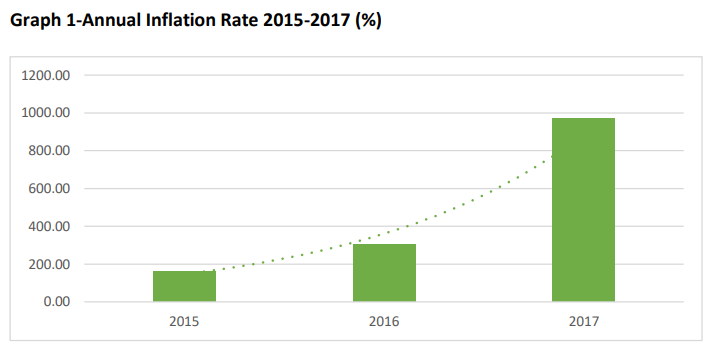
\includegraphics[width=0.8\textwidth]{images/1.1.png}
\caption{Графік 1-річний рівень інфляції 2015-2017 (\%) -- пер. з англ. [4]}
\label{fig:weimar}
\end{figure}

Рис. 1.1 відображає графік Graph 1-Annual Inflation Rate 2015-2017 (\%) (Графік 1 – Річний рівень інфляції 2015-2017 рр. (\%)), по горизонталі рік, по вертикалі відсоток CPI рік-до-року. З графіку можна побачити, що CPI у 2015 р. складав приблизно 200\%, 2016 - $\approx350\%$, 2017 - $\approx1000\%$.

Окремо варто розглянути поняття стагфляції -- стану, за якого висока інфляція поєднується зі стагнацією економіки та зростанням безробіття. Стагфляція є особливо небезпечною, оскільки традиційні монетарні інструменти боротьби з інфляцією, наприклад підвищення відсоткових ставок, поглиблюють економічний спад, тоді як стимулюючі заходи для виходу з рецесії посилюють інфляцію~[2].

\subsection{Чинники, що впливають на інфляцію}

Інфляція є багатофакторним явищем, і розуміння її рушійних сил є необхідним для економічного аналізу і прогнозування. Прийнято виділяти кілька груп чинників: чинники попиту, чинники пропозиції, монетарні чинники, інфляційні очікування й зовнішні фактори~[2]. На практиці ці групи тісно взаємодіють між собою, і така множинна взаємодія робить задачу прогнозування інфляції складною через наявність великої сукупності різнорідних факторів.

Інфляція попиту виникає, коли сукупний попит в економіці перевищує її виробничі можливості. Якщо рівень зайнятості та доходів населення зростає, споживачі мають більше грошей і прагнуть витратити їх на товари та послуги; коли виробнича система не здатна у короткостроковому періоді наростити пропозицію відповідними темпами, продавці підвищують ціни~[2].

Інфляція пропозиції виникає, коли зростання витрат виробництва змушує підприємства підвищувати ціни на кінцеву продукцію. Основними чинниками тут є зростання цін на енергоносії, підвищення вартості сировини та матеріалів, зростання заробітних плат, а також підвищення транспортних витрат~[2].

Монетарні чинники пов'язані з кількістю грошей в обігу та швидкістю їх обертання. Кількісна теорія грошей описується класичним рівнянням обміну Фішера:

\begin{equation*}
M \times V = P \times Y,
\end{equation*}

\noindentде $M$ -- грошова маса в обігу; $V$ -- швидкість обертання грошей; $P$ -- загальний рівень цін; $Y$ -- реальний обсяг виробництва (реальний валовий внутрішній продукт, ВВП). За припущення про відносну стабільність~$V$ у короткостроковому періоді, темп зростання грошової маси, що перевищує темп зростання реального виробництва, у довгостроковому плані визначає темп інфляції~[2]. У крайньому випадку, коли уряд вдається до фінансування бюджетного дефіциту шляхом емісії, виникає ризик гіперінфляції. Саме тому в провідних країнах центральні банки є юридично незалежними від виконавчої влади установами~[3].

Інфляційні очікування -- це суб'єктивні уявлення домогосподарств, підприємств, інвесторів тощо про майбутню інфляцію. Попри свій суб'єктивний характер, вони мають цілком реальний вплив на ціни: якщо підприємці очікують зростання цін на сировину, вони закладають це зростання у власні ціни заздалегідь; якщо працівники очікують інфляцію, вони вимагають підвищення заробітних плат, що знову ж таки збільшує витрати виробництва і підштовхує ціни~[2]. Управління інфляційними очікуваннями є одним із ключових завдань сучасних центральних банків.

Зовнішні чинники відіграють особливо значну роль у малих відкритих економіках, до яких належить й Україна. Зміна обмінного курсу є одним із найвпливовіших чинників: девальвація національної валюти автоматично підвищує ціни на імпортні товари, що прямо впливає на споживчий кошик. Цей механізм у літературі позначається як ефект перенесення і кількісно описується еластичністю:

\begin{equation}\label{eq:pass_through}
\varepsilon = \frac{\Delta P/P}{\Delta E/E},
\end{equation}

\noindentде $\varepsilon$ -- еластичність перенесення; $\Delta P/P$ -- відносна зміна цін; $\Delta E/E$ -- відносна зміна обмінного курсу. Для України, як і для більшості малих відкритих економік, $\varepsilon$ зазвичай знаходиться в діапазоні 0,2-0,4, що означає: 10-відсоткова девальвація гривні веде в середньому до 2-4-відсоткового зростання споживчих цін протягом наступних 6-12 місяців~[5].

\subsection{Інфляція в Україні}

Розглядаючи інфляційну історію України, важливо зосередитись на ключових подіях, що формують контекст для побудови прогностичних моделей.

Перший період -- гіперінфляція початку 1990-х. Лібералізація цін у 1992 році спричинила інфляцію близько 2~000\%, а у 1993 році інфляція зросла до 10~256\%~[6]. Основним чинником була масштабна кредитна емісія НБУ для покриття бюджетного дефіциту, що досягав 12,2\% ВВП~[2].

\begin{figure}[ht]
\centering
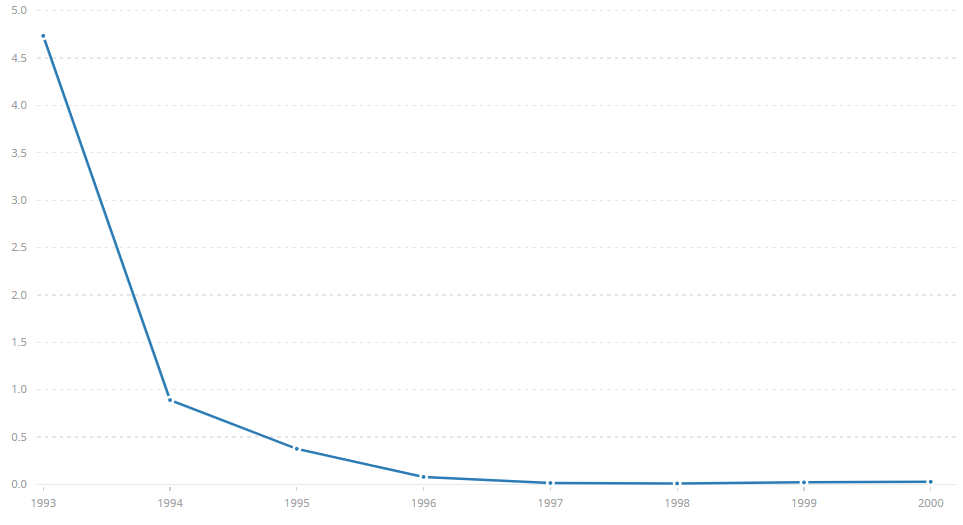
\includegraphics[width=0.8\textwidth]{images/1.2.png}
\caption{Динаміка інфляції в Україні (CPI) з 1993 по 2000~рр. По вертикалі - тисячі \%, по горизонталі - рік.}
\label{fig:ukraine_inflation_1}
\end{figure}

Другий період -- час відносної стабільності 2000-х років (інфляція в межах 6-16\% на рік). На перший погляд, цей період міг би слугувати ідеальним матеріалом для побудови прогнозних моделей. Однак дослідження показують, що значною мірою стабільність забезпечувалася штучним утриманням обмінного курсу гривні на рівні близько 8~грн/дол. -- кроком, що поступово накопичував зовнішні дисбаланси~[8]. Коли у 2014-2015 роках утримання курсу стало неможливим, корекція мала досить негативні наслідки: інфляція у 2015~р. досягла 48,7\%, а девальвація гривні склала близько 67\%~[7]. Цей епізод демонструє важливу властивість української інфляції -- її чутливість до структурних змін у режимі обмінного курсу.

Третій період - час після початку повномасштабного вторгнення Росії у лютому 2022~р. Руйнування виробничих потужностей та логістичної інфраструктури різко скоротили пропозицію товарів, мільйони вимушених переселенців змінили географію попиту, масштабне фінансування воєнних витрат створило додатковий тиск на бюджет, а НБУ був змушений підвищити облікову ставку до 25\% -- рекордного рівня~[8]. Інфляція у 2022~р. сягнула близько 26,6\%~[5].

\begin{figure}[ht]
\centering
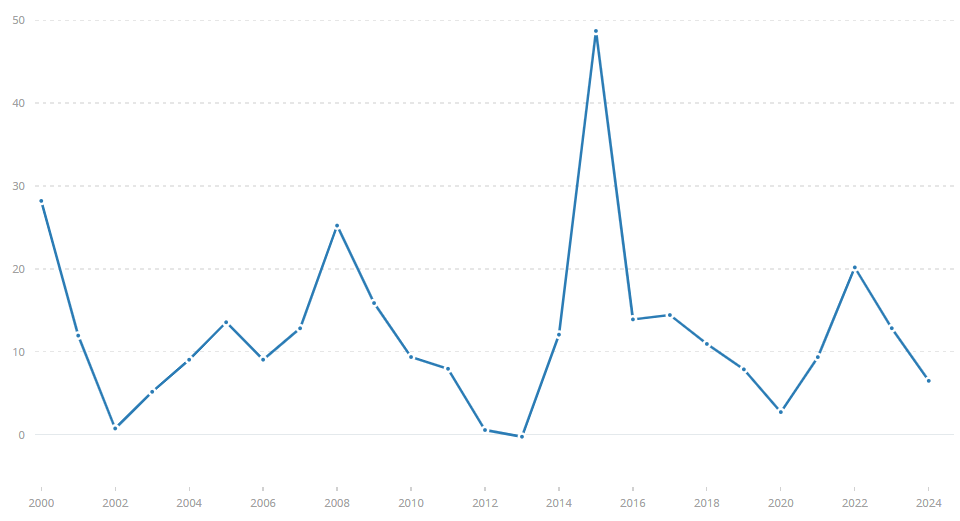
\includegraphics[width=0.8\textwidth]{images/1.3.png}
\caption{Динаміка інфляції в Україні (CPI) з 2000 по 2024~рр. По вертикалі - \%, по горизонталі - рік.}
\label{fig:ukraine_inflation_2}
\end{figure}

Узагальнюючи наведені факти, можна сформулювати кілька ключових вимог до прогностичної моделі: (1)~здатність працювати в умовах нестаціонарності та структурних зрушень, (2)~урахування широкого спектру чинників, (3)~можливість швидкої адаптації до нових режимів економічної політики, (4)~інтерпретованість результатів для чіткого розуміння причин. Такі вимоги обумовлюють перехід від класичних математичних моделей до методів машинного навчання та штучного інтелекту (ШІ).

\subsection{Антиінфляційна політика та таргетування інфляції в Україні}

Розуміння антиінфляційної політики центрального банку та інструментів, за допомогою яких він здійснює вплив на інфляцію, дозволяє правильно інтерпретувати прогнози та визначати їх практичну цінність. В свою чергу, розуміння інструментів впливу на інфляцію дозволяє підбирати правильні метрики для навчання моделі, що будуть насправді відображати стан економіки, й навпаки, розуміти, які дані використовувати не слід через їхню незастосовність в теперішніх умовах.

Основним інструментом монетарної політики є ключова ставка центрального банку. Підвищуючи її, регулятор робить запозичення дорожчими, тому банки отримують ресурси за вищою ціною і відповідно підвищують ставки за кредитами для бізнесу та населення~[3]. Це знижує попит на кредити, скорочує інвестиції та споживчі витрати, і зрештою знижує тиск на ціни. Зв'язок між реальною відсотковою ставкою та номінальною описується ефектом Фішера:

\begin{equation*}
r \approx i - \pi^e,
\end{equation*}

\noindentде $r$ -- реальна відсоткова ставка; $i$ -- номінальна відсоткова ставка (наприклад, облікова ставка центрального банку); $\pi^e$ -- очікуваний рівень інфляції. Ця формула пояснює, чому центральні банки зазвичай встановлюють номінальну ставку вищою за поточну і прогнозовану інфляцію -- щоб реальна ставка залишалась додатною і стимулювала заощадження у національній валюті~[9].

Досить важливим моментом у монетарній політиці стало запровадження режиму інфляційного таргетування. Суть підходу полягає у тому, що центральний банк публічно оголошує конкретний цільовий рівень інфляції і підпорядковує усю свою монетарну політику досягненню цієї мети~[3]. Інфляційне таргетування має кілька суттєвих переваг: публічний орієнтир дозволяє зафіксувати інфляційні очікування, підвищує передбачуваність політики та захищає центральний банк від короткострокового політичного тиску.

В Україні режим інфляційного таргетування було запроваджено у 2015 році -- у складних макроекономічних умовах: країна перебувала у стані збройного конфлікту, економіка падала, банківська система потерпала від масового виведення депозитів, а гривня щойно пережила різку девальвацію~[10]. Тим не менш, реформа дала помітні результати: у 2017 році інфляція склала 13,7\%, у 2018-му -- 9,8\%, у 2019-му -- 4,1\%~[11], тобто вперше за довгий час опинилась нижче офіційної цілі НБУ.

Поточна ціль НБУ становить 5\% з допустимим інтервалом $\pm$1~п.п.~[12]. Згідно з Інфляційним звітом за січень 2026~р., монетарна політика спрямована на приведення інфляції до цієї цілі на горизонті, що не перевищує трьох років. Прогноз НБУ передбачає зниження інфляції до 7,5\% у 2026~р., до 6\% у 2027-му та досягнення цільових 5\% у 2028~р.~[12].

Однак дослідники зазначають, що механізми монетарної трансмісії в Україні залишаються відносно слабкими порівняно з розвиненими ринками~[13]. Це означає, що зміна облікової ставки не так швидко і повно відображається на кредитних ставках та сукупному попиті, як у країнах Європейського Союзу (ЄС). Однією з причин є низький рівень кредитування економіки приватним сектором. Слабкість механізмів трансмісії в українській економіці -- додатковий аргумент на користь прогностичних моделей, що враховують широкий спектр різнорідних чинників.

\section{Прогнозування та моделювання інфляції}

Розвиток кількісних методів прогнозування інфляції тривав упродовж усього XX~ст. і сформував широкий спектр інструментів, що нині позначаються як \textit{класичні}. До них відносять регресійні моделі, моделі авторегресії, векторні авторегресії, структурні макроекономічні моделі та моделі на основі кривої Філліпса. Кожен з цих підходів має власну теоретичну базу, переваги й обмеження, а також -- що особливо важливо для контексту даної роботи -- спільне принципове обмеження, яке і обумовлює перехід до сучасних методів.

\subsection{Класичні підходи до прогнозування інфляції}

Одним з найбільш широко застосовуваних класів моделей є моделі авторегресії проінтегрованого ковзного середнього -- ARIMA (Autoregressive Integrated Moving Average). Теорія цих моделей закладено в роботі~[14], яка запропонувала систематичну методологію ідентифікації, оцінювання та верифікації моделей часових рядів. У загальному вигляді модель ARIMA описується рівнянням:

\begin{equation*}
y_t = c + \varphi_1 y_{t-1} + \ldots + \varphi_p y_{t-p}
      + \varepsilon_t + \theta_1\varepsilon_{t-1} + \ldots + \theta_q\varepsilon_{t-q},
\end{equation*}

\noindentде $y_t$ -- поточне значення часового ряду; $c$ -- константа; $\varphi_1,\ldots,\varphi_p$ -- коефіцієнти авторегресійної складової порядку~$p$; $\theta_1,\ldots,\theta_q$ -- коефіцієнти ковзного середнього порядку~$q$; $\varepsilon_t$ -- випадкова похибка у момент~$t$. Параметр~$d$ позначає кількість взять різниць, необхідну для досягнення стаціонарності~[15].

Головною перевагою ARIMA є те, що для побудови моделі достатньо лише одного часового ряду -- самого показника інфляції. Не потрібно збирати та підтримувати в актуальному стані великий масив допоміжних даних. Дослідження ірландської~[17], кенійської~[18], руандійської~[15] та сьєрра-леонської~[19] інфляції підтвердили, що моделі ARIMA дають задовільні результати на коротких горизонтах прогнозування -- до трьох-шести місяців -- у стабільних економічних умовах. Однак ARIMA повністю ігнорує будь-які зовнішні чинники -- рух обмінного курсу, зміни у грошовій масі, цінові шоки на сировинних ринках. Якщо відбуваються структурні зрушення, прогнози різко погіршуються~[16].

Розширенням ARIMA є модель SARIMA (Seasonal ARIMA), що додатково включає сезонні компоненти. Для інфляції, яка часто демонструє стійкі сезонні патерни (наприклад, через урожаї або тарифні перегляди), SARIMA є більш точною. На практиці SARIMA є одним із найбільш стійких бенчмарків при прогнозуванні споживчих цін і широко застосовується у дослідженнях центральних банків~[16].

Принципово іншим класом є векторні авторегресійні моделі -- VAR (Vector Autoregression). На відміну від ARIMA, що є моделлю одного ряду, VAR одночасно моделює систему взаємозалежних змінних. У системі VAR кожна змінна описується як лінійна функція власних минулих значень та минулих значень усіх інших змінних моделі. Для прогнозування інфляції типовими змінними VAR є: інфляція, ВВП, відсоткова ставка, обмінний курс, грошова маса, ціни на нафту~[19].

VAR модель здатна враховувати взаємозворотні причинно-наслідкові зв'язки між змінними і є потужним інструментом для сценарного аналізу. Водночас класичні VAR моделі страждають на прокляття розмірності (curse of dimensionality): з ростом числа змінних та лагів кількість параметрів, що підлягають оцінюванню, зростає квадратично~[15]. Відповіддю на цю проблему стала байєсівська векторна авторегресія (Bayesian Vector Autoregression, BVAR). BVAR моделі широко застосовуються центральними банками, у тому числі Федеральною резервною системою США (ФРС) та Європейським центральним банком (ЄЦБ)~[16].

Окремий важливий клас становлять моделі на основі кривої Філліпса, яка відображає залежність між рівнем безробіття та рівнем інфляції. Пізніші розробки ввели в модель роль інфляційних очікувань. Однак починаючи з 1990-х років прогнози суттєво погіршали, адже зв'язок між безробіттям та інфляцією значно ослаб (так зване «сплющення» кривої Філіпса)~[16].

Найбільш структурно завершеним класом є динамічні стохастичні моделі загальної рівноваги -- DSGE (Dynamic Stochastic General Equilibrium). DSGE моделі ґрунтуються на мікроекономічних засадах і є основою прогнозних систем більшості великих центральних банків~[15]. Вони мають сильну теоретичну інтерпретованість, проте вимагають значної кількості теоретичних припущень і нерідко поступаються BVAR у точності~[16].

Спільне принципове обмеження більшості класичних методів -- лінійність припущень. Вони погано вловлюють нелінійні взаємозалежності, що є характерними для реальних інфляційних процесів, особливо під час криз і структурних зрушень~[20].

\subsection{Сучасні підходи: машинне навчання у прогнозуванні інфляції}

Серед алгоритмів ML широко розповсюдженими є ансамблеві методи на основі дерев рішень. Метод випадкового лісу (Random Forest, RF) будує велику кількість дерев рішень на різних підвибірках даних і різних підмножинах ознак, а кінцевий прогноз формується шляхом усереднення. Хоча дослідження~[21] показало, що Random Forest перевершує класичні бенчмарки при прогнозуванні інфляції в США на основі понад 100 макроекономічних змінних, особливо у нестабільні економічні періоди.

Градієнтний бустинг (Gradient Boosting, GB) та його найвідоміша реалізація -- XGBoost (Extreme Gradient Boosting) -- є ще одним потужним ансамблевим методом. На відміну від RF, що будує дерева паралельно, бустинг навчає їх послідовно: кожне наступне дерево зосереджується на прикладах, де попередня ансамблева модель помилилась найбільше~[22]. Робота Міжнародного валютного фонду (МВФ) 2024~р. <<Mending the Crystal Ball>> демонструє, що ансамблеві ML-методи здатні суттєво покращити прогнозування базової інфляції на горизонтах від 1 до 6~місяців. При цьому якість прогнозу особливо зростає у ті моменти, коли стандартні економічні залежності порушуються через нестандартні шоки -- саме там, де класичні методи найбільш вразливі~[22].

Регуляризовані лінійні моделі -- LASSO (Least Absolute Shrinkage and Selection Operator), Ridge-регресія та їхнє поєднання Elastic Net -- займають проміжне місце між класичними лінійними методами та складнішими алгоритмами ML. LASSO мінімізує функцію втрат із додаванням штрафу за $L_1$-норму вектора коефіцієнтів:

\begin{equation*}
L(\beta) = \sum_{i=1}^{n}(y_i - \hat{y}_i)^2 + \lambda\sum_{j=1}^{p}|\beta_j|,
\end{equation*}

\noindentде $\beta$ -- вектор коефіцієнтів; $y_i$,~$\hat{y}_i$ -- спостережене та прогнозоване значення; $\lambda$ -- параметр регуляризації, що контролює силу штрафу. Завдяки $L_1$-штрафу LASSO автоматично обнуляє менш важливі предиктори і тим самим виконує відбір змінних~[22]. За великої кількості потенційних предикторів LASSO є ефективним інструментом для приведення моделі до найбільш інформативної підмножини. Деякі дослідження показують, що LASSO-регресія нерідко конкурентоспроможна з глибокими нейромережевими моделями, особливо на коротших горизонтах прогнозування~[16].

Нейронні мережі і глибоке навчання відкривають широкі можливості для моделювання нелінійних залежностей. Особливу роль у роботі з часовими рядами відіграє архітектура рекурентних нейронних мереж, зокрема мереж з довготривалою і короткотривалою пам'яттю -- LSTM (Long Short-Term Memory). Завдяки спеціальній архітектурі комірок пам'яті з вентилями LSTM здатна зберігати і передавати інформацію через великі часові проміжки~[16]. Однак практичні результати застосування LSTM до прогнозування інфляції є неоднозначними. Ряд досліджень фіксує, що LSTM поступається простішим моделям -- SARIMA, Random Forest або навіть LASSO -- особливо на коротких горизонтах~[16].

Останніми роками увагу привертають архітектури на основі механізму уваги і трансформери. На відміну від LSTM, що обробляє послідовність покроково, трансформер розглядає всю послідовність одразу і явно зважує взаємозалежності між різними часовими точками~[23].

Жоден з описаних методів не є безумовно найкращим у всіх ситуаціях, а вибір залежить від горизонту прогнозування, обсягу й якості даних, а також наявності структурних зрушень. Однак ансамблеві деревні методи (особливо XGBoost та RF) є найбільш збалансованим вибором для задач макроекономічного прогнозування з обмеженим обсягом даних -- поєднуючи високу точність, відносну стабільність та можливість інтерпретації результатів.

\subsection{Пояснювальний штучний інтелект та метод SHAP}

Висока точність прогнозів сама по собі не вирішує всіх проблем -- без можливості пояснити, чому модель видає той чи інший результат, її практична цінність для прийняття рішень дуже обмежена. Особливо це стосується макроекономічного прогнозування, адже центральний банк, що ухвалює рішення про підвищення облікової ставки, має обґрунтувати своє рішення. Саме тому XAI є невід'ємним компонентом сучасного підходу до моделювання інфляції.

Серед методів XAI на сьогодні найбільш теоретично обґрунтованим є SHAP (SHapley Additive exPlanations)~[24]. SHAP базується на концепції значень Шеплі -- підході з теорії кооперативних ігор. Якщо розглядати ознаки моделі як <<гравців>>, що спільно роблять <<прогноз-виграш>>, то значення Шеплі вказує, яким повинен бути справедливий розподіл цього виграшу між гравцями.

Формально, SHAP-значення ознаки~$i$ для конкретного спостереження визначається як:

\begin{equation*}
\varphi_i = \sum_{S\subseteq N\setminus\{i\}}
\frac{|S|!\,(|N|-|S|-1)!}{|N|!}
\bigl[f(S\cup\{i\})-f(S)\bigr],
\end{equation*}

\noindentде $\varphi_i$ -- SHAP-значення ознаки~$i$; $N$ -- повна множина ознак моделі; $S$ -- підмножина ознак, що не містить~$i$; $|S|$ та~$|N|$ -- розміри відповідних множин; $f(S)$ -- прогноз моделі при використанні лише ознак з~$S$~[25]. Інтуїтивно ця формула описує середній маржинальний внесок ознаки~$i$, обчислений по всіх можливих підмножинах інших ознак.

SHAP надає два рівні пояснень -- локальний та глобальний. На локальному рівні для кожного окремого прогнозу можна обчислити, який внесок зробила кожна ознака. На глобальному рівні SHAP-значення можна агрегувати по всіх спостереженнях, щоб зрозуміти, які ознаки в цілому є найбільш важливими і як вони впливають на прогнози~[26].

Технічно для деревних ансамблевих моделей (Random Forest, XGBoost, LightGBM) існує спеціалізована ефективна реалізація -- TreeSHAP, що дозволяє обчислювати точні SHAP-значення з обчислювальною складністю $O(TLD^2)$ замість $O(TL \cdot 2^M)$ для загального випадку, де $T$ -- кількість дерев, $L$ -- максимальна кількість листків, $D$ -- глибина, $M$ -- кількість ознак~[25]. Ця ефективність робить SHAP практично застосовним навіть для великих ансамблевих моделей з десятками ознак.

У контексті прогнозування інфляції SHAP має додаткові важливі переваги. Він дозволяє відстежувати у часі, як змінюється відносна важливість різних чинників, адже у різні економічні режими ключову роль можуть відігравати різні змінні. Також SHAP-аналіз можна використовувати як інструмент сценарного моделювання для аналізу можливих майбутніх сценаріїв при зміні того чи іншого показника~[27].

Поєднання сучасних точних методів машинного навчання з прозорим поясненням робить прогнозування якісно новим у порівнянні як з класичними економетричними моделями, так і з важкоінтерпретованими підходами ML.

\subsection{Дані: проблема обмеженості та залучення країн-аналогів}

Якість будь-якої прогностичної моделі, особливо побудованої на методах машинного навчання, визначається не лише вибором алгоритму, а й якістю та обсягом доступних даних. Для української макроекономіки питання даних є одним з найбільш проблемних.

Перша проблема -- обмежений часовий горизонт однорідних даних. Як було показано у підрозділі~1.1.3, інфляційний ряд України до 1996 року є аномальним через гіперінфляцію і фактично не може бути використаний для побудови моделей, що мають прогнозувати сучасні значення. Період 1996-2014 рр. є відносно стабільним, але характеризується режимом обмінного курсу, прив’язаного до долара США, який після 2014 року було замінено інфляційним таргетуванням. Таким чином, реально придатний для побудови сучасних ML моделей період охоплює близько 10-11 років, або приблизно 120-130 місячних спостережень~[11]. Для класичних статистичних моделей такий обсяг є достатнім, але для алгоритмів машинного навчання - ні.

Друга проблема -- нестаціонарність та структурні зрушення у самих даних. Серед цих 120-130 спостережень частина припадає на період пандемії COVID-19 (2020-2021~рр.), частина - на повномасштабну війну (з 2022~р.), що супроводжується безпрецедентними шоками всіх типів. Кожен такий проміжок фактично створює новий режим, що знижує ефективність навчання моделі на історичних даних попередніх режимів.

Третя проблема -- обмежений набір предикторів з достатньою глибиною. Для багатьох важливих макроекономічних показників в Україні часові ряди починаються занадто пізно (2010-ті рр.) або завершуються занадто рано та не публікуються останні декілька років.

В такому випадку для подолання обмеженості даних є логічним збільшення вибірки за рахунок включення схожих спостережень. У контексті макроекономіки це означає залучення даних інших країн, що мають подібні структурні характеристики. У даній роботі такими країнами-аналогами обрано Латвію та Литву. Цей вибір обумовлений кількома взаємопов'язаними причинами.

Латвія, Литва та Україна пройшли спільний шлях трансформації від радянської командної економіки до ринкової. Усі три країни на початку 1990-х пережили періоди екстремально високої інфляції: Латвія -- 958,6\%~[27], Литва -- 1~100\%~[27], Україна -- 10~256\%~[6]. Усі три відновили самостійні центральні банки, провели грошові реформи (Литва ввела літас у 1993~р., Латвія -- лат у 1993-му, Україна -- гривню у 1996-му). Це означає принципову подібність структурних викликів у монетарній сфері.

Латвія та Литва, як і Україна, є малими відкритими економіками з високою чутливістю до зовнішніх шоків -- насамперед курсових та сировинних. У всіх трьох країнах ефект перенесення обмінного курсу відіграє ключову роль у формуванні інфляційної динаміки~[28].

У 2022~р., коли Україна зіткнулася з повномасштабним російським вторгненням, інфляція в Латвії досягла 17,2\%, у Литві -- 18,9\%~[28]. Хоча природа шоків була різною (для України -- пряма війна, для країн Балтії -- енергетичні наслідки відмови від російських енергоносіїв та геополітичні ризики), макроекономічна динаміка в усіх трьох країнах продемонструвала якісно подібні патерни: різке зростання цін на енергоносії, девальваційний (для України) або інфляційний (для країн єврозони) тиск, жорсткість монетарної політики у відповідь.

Латвія і Литва мають значно довші та якісніші ряди макроекономічних даних. Їхнє членство в ЄС забезпечило стандартизацію статистики за методологією Eurostat, тривалу історію інфляційного таргетування та повне розкриття даних. Це дозволяє суттєво розширити навчальну вибірку, додавши до приблизно 130 українських спостережень ще близько 250-300 спостережень з кожної з двох балтійських країн.

\chapconclude{1}

У цьому розділі було обґрунтовано актуальність проблеми інфляції у всі часи та складність прогнозування цього економічного процесу через його мультифакторність та чутливість до великої кількості чинників. Були розглянуті класичні підходи прогнозування, зокрема моделі ARIMA, та сучасні ML рішення, зокрема XGBoost. Також було обґрунтовано важливість впровадження XAI для практичного використання сучасних моделей з використанням методів машинного навчання для розуміння ключових факторів що мали вплив на той чи інший прогноз та винесення відповідного рішення для стримування інфляції.

Для проведення власного експерименту обрані моделі ARIMA, XGBoost та SHAP. Математичні засади та теоретичне обгрунтування моделі буде наведено в наступному розділі.

\chapter{Теоретичні засади гібридної моделі прогнозування}

У цьому розділі описано математичні засади гібридної моделі на основі ARIMA, XGBoost та SHAP. Поєднання цих трьох підходів дозволяє використати сильні сторони кожного з них: ARIMA є перевіреним і простим й вловлює лінійну складову часового ряду інфляції; XGBoost моделює нелінійність зовнішніх чинників; SHAP надає кількісну оцінку внеску кожного фактора у прогноз роблячи модель інтерпретованою.

\section{Прогнозування часових рядів з використанням ARIMA}

Часовим рядом називають послідовність спостережень $\{z_t\}$ певної величини, зафіксованих у дискретні рівновіддалені моменти часу $t = 1, 2, \ldots, n$. У контексті цієї роботи $z_t$ -- місячне значення річної інфляції в Україні.

Ключова особливість аналізу часових рядів полягає в тому, що послідовні спостереження не є статистично незалежними, тобто значення $z_t$ корелює з попередніми значеннями $z_{t-1}, z_{t-2}, \ldots$. Саме наявність часової структури залежностей і є основою для прогнозування: якщо в ряді присутні стійкі залежності, то поточне значення $z_t$ містить інформацію про майбутнє значення $z_{t+l}$ через лаг~$l$.

Завдання прогнозування полягає в побудові функції прогнозу $\hat{z}_t(l)$ -- оцінки значення $z_{t+l}$, побудованої на момент~$t$ за всіма доступними попередніми спостереженнями $z_t, z_{t-1}, z_{t-2}, \ldots$. Оптимальною з погляду середньоквадратичної помилки вважається функція, що мінімізує математичне сподівання $E[(z_{t+l} $-$ \hat{z}_t(l))^2]$ для кожного лагу~$l$~[14].

Базовою концепцією, що дозволяє єдиним чином описати широкий клас стохастичних моделей часових рядів, є модель лінійного фільтра. У ній ряд $z_t$ розглядається як вихід лінійного перетворення білого шуму -- послідовності некорельованих випадкових величин $\{a_t\}$ з нульовим середнім і сталою дисперсією $\sigma_a^2$:

\begin{equation*}
z_t = \mu + a_t + \psi_1 a_{t-1} + \psi_2 a_{t-2} + \ldots = \mu + \psi(B) a_t,
\end{equation*}

\noindentде $\mu$ -- рівень процесу; $\psi_1, \psi_2, \ldots$ -- коефіцієнти лінійного фільтра; $B$ -- оператор зсуву, що визначається як $B z_t = z_{t-1}$~[14].

Стохастичний процес $\{z_t\}$ називається строго стаціонарним, якщо спільний розподіл будь-якого набору $z_{t_1}, z_{t_2}, \ldots, z_{t_k}$ збігається зі спільним розподілом $z_{t_1+h}, z_{t_2+h}, \ldots, z_{t_k+h}$ для будь-якого зсуву~$h$. У практичних задачах прогнозування достатньо слабкішої умови стаціонарності у широкому сенсі (другого порядку), за якої сталими в часі є перші два моменти процесу~[14]:

\begin{equation*}
E[z_t] = \mu = \text{const}, \quad \operatorname{Var}(z_t) = \sigma_z^2 = \text{const}, \quad \operatorname{Cov}(z_t, z_{t+k}) = \gamma_k,
\end{equation*}

\noindentтобто математичне сподівання та дисперсія не залежать від~$t$, а коваріаційна функція $\gamma_k$ залежить лише від лагу~$k$, але не від моменту~$t$. За цих умов автокореляційна функція має вигляд:

\begin{equation}\label{eq:acf}
\rho_k = \frac{\gamma_k}{\gamma_0} = \frac{\operatorname{Cov}(z_t, z_{t+k})}{\operatorname{Var}(z_t)}.
\end{equation}

Стаціонарність є фундаментальною передумовою для застосування моделей AR, MA та ARMA. Якщо вона порушується -- а більшість макроекономічних рядів, у тому числі ряди інфляції, у сирому вигляді нестаціонарні -- необхідно приводити ряд до стаціонарного. Ця властивість і є у моделях ARIMA: у них нестаціонарність обробляється через операцію диференціювання.

\subsection{Стаціонарність часових рядів}

Як було зазначено вище, стаціонарність ряду є необхідною умовою для застосування моделей класу AR, MA та ARMA. Перш ніж формалізувати самі моделі, доцільно розглянути, як перевіряти стаціонарність ряду та як приводити нестаціонарний ряд до стаціонарного -- така операція приведення визначає параметр~$d$ у моделі ARIMA($p$,$d$,$q$).

Найбільш поширеним типом нестаціонарності в макроекономічних рядах є наявність одиничного кореня. Наприклад наведено авторегресійний процес першого порядку:

\begin{equation*}
z_t = \phi z_{t-1} + a_t,
\end{equation*}

\noindentде $a_t$ -- білий шум. Стаціонарність такого процесу залежить від значення~$\phi$: за умови $|\phi| < 1$ процес стаціонарний, а за $\phi = 1$ ряд перетворюється на нестаціонарне випадкове блукання $z_t = z_{t-1} + a_t$: його дисперсія зростає лінійно з~$t$, а вплив минулих шоків не згасає [14].

Для перевірки наявності одиничного кореня використовують розширений тест Дікі-Фуллера (Augmented Dickey-Fuller, ADF). Тестова регресія має вигляд:

\begin{equation*}
\Delta z_t = \alpha + \beta t + \rho z_{t-1} + \sum_{i=1}^{k} \delta_i \Delta z_{t-i} + a_t,
\end{equation*}

\noindentде $\Delta z_t = z_t - z_{t-1}$ -- перша різниця ряду; $\alpha$ -- константа; $\beta t$ -- детермінований тренд; $\rho$ -- ключовий коефіцієнт, відповідальний за наявність одиничного кореня; $k$ -- кількість лагів першої різниці~[14].

Тест перевіряє нульову гіпотезу про наявність одиничного кореня:
\begin{equation*}
H_0: \rho = 0 \quad (\text{ряд нестаціонарний}) \quad \text{проти} \quad H_1: \rho < 0 \quad (\text{ряд стаціонарний}).
\end{equation*}

Якщо обчислена $t$-статистика для коефіцієнта~$\rho$ менша за критичне значення, нульова гіпотеза відхиляється і ряд приймається як стаціонарний. У протилежному випадку -- ряд містить одиничний корінь і потребує диференціювання.

Якщо тест ADF не дозволяє відхилити~$H_0$, ряд приводиться до стаціонарного шляхом застосування оператора диференціювання $\nabla = 1 - B$:

\begin{equation*}
\nabla z_t = z_t - z_{t-1}.
\end{equation*}

У більшості випадків однократного диференціювання достатньо для досягнення стаціонарності. Якщо отриманий ряд $\nabla z_t$ все ще не пройшов тест ADF, застосовується диференціювання другого порядку $\nabla^2 z_t = \nabla(\nabla z_t)$. Кількість послідовних застосувань оператора диференціювання, необхідних для приведення ряду до стаціонарного, і визначає параметр~$d$ у моделі ARIMA($p$,$d$,$q$). Для більшості макроекономічних рядів, у тому числі для рядів інфляції в малих відкритих економіках, типовим значенням є $d = 1$, рідше $d = 0$ (якщо ряд стаціонарний у сирому вигляді) або $d = 2$~[14].


\subsection{AR, MA, ARMA та ARIMA моделі}

Серед сімейства моделей лінійного фільтра виділяють два важливі окремі класи: авторегресійні моделі та моделі ковзного середнього. Їх поєднання утворює модель ARMA, а додавання операції диференціювання -- модель ARIMA.

Авторегресійним процесом порядку~$p$ (AR($p$)) називають процес, у якому поточне значення ряду виражається як лінійна комбінація~$p$ попередніх значень та поточної випадкової похибки:

\begin{equation*}
z_t = c + \phi_1 z_{t-1} + \phi_2 z_{t-2} + \ldots + \phi_p z_{t-p} + a_t,
\end{equation*}

\noindentде $\phi_1, \ldots, \phi_p$ -- коефіцієнти авторегресії; $c$ -- константа, пов'язана з рівнем процесу; $a_t$ -- білий шум з нульовим середнім і сталою дисперсією~$\sigma_a^2$~[14]. Через оператор зсуву~$B$ модель AR($p$) записується компактно:

\begin{equation*}
\Phi(B) z_t = c + a_t, \quad \text{де} \quad \Phi(B) = 1 - \phi_1 B - \phi_2 B^2 - \ldots - \phi_p B^p.
\end{equation*}

Поліном $\Phi(B)$ називається авторегресійним поліномом, а його порядок~$p$ -- порядком авторегресії~[14].

Процес ковзного середнього порядку~$q$ (MA($q$)) виражає поточне значення ряду як лінійну комбінацію поточної та~$q$ попередніх випадкових похибок:

\begin{equation*}
z_t = \mu + a_t + \theta_1 a_{t-1} + \theta_2 a_{t-2} + \ldots + \theta_q a_{t-q},
\end{equation*}

\noindentде $\theta_1, \ldots, \theta_q$ -- коефіцієнти ковзного середнього; $\mu$ -- математичне сподівання процесу. У компактному вигляді:

\begin{equation*}
z_t = \mu + \Theta(B) a_t, \quad \text{де} \quad \Theta(B) = 1 + \theta_1 B + \theta_2 B^2 + \ldots + \theta_q B^q.
\end{equation*}

Поліном $\Theta(B)$ називається поліномом ковзного середнього. На відміну від AR-процесу, MA-процес стаціонарний завжди, незалежно від значень коефіцієнтів~$\theta_j$. Натомість для нього висувається інша вимога -- \textbf{умова оборотності}: усі корені рівняння $\Theta(B) = 0$ повинні лежати поза одиничним колом~[14].

Об'єднання обох концепцій дає змішану модель авторегресії - ковзного середнього порядку $(p, q)$, що позначається ARMA($p$,$q$):

\begin{equation*}
\Phi(B) z_t = c + \Theta(B) a_t.
\end{equation*}

ARMA модель здатна описувати ширший клас стаціонарних процесів, ніж AR або MA окремо, при цьому, як правило, з меншою кількістю параметрів.

Однак ARMA моделі застосовні лише до стаціонарних рядів. Для нестаціонарних рядів, що приводяться до стаціонарних через $d$-кратне диференціювання, використовується модель ARIMA($p$,$d$,$q$), що в операторному вигляді записується як:

\begin{equation}\label{eq:arima_model}
\Phi(B) (1 - B)^d z_t = c + \Theta(B) a_t,
\end{equation}

\noindentде множник $(1 - B)^d = \nabla^d$ реалізує операцію $d$-кратного взяття різниці~[14]. Розгорнуто, для випадку $d = 1$, який є найпоширенішим для рядів інфляції, модель набуває вигляду:

\begin{equation*}
\Delta z_t = c + \phi_1 \Delta z_{t-1} + \ldots + \phi_p \Delta z_{t-p} + a_t + \theta_1 a_{t-1} + \ldots + \theta_q a_{t-q},
\end{equation*}

\noindentтобто ARIMA($p$,1,$q$) -- це фактично ARMA($p$,$q$), застосована не до самого ряду $z_t$, а до його перших різниць $\Delta z_t$.

Гнучкість трипараметричної форми ARIMA($p$,$d$,$q$) дозволяє покривати широкий спектр часових рядів за допомогою єдиного формального апарату, що обгрунтовує її широке використання у прогнозування часових рядів.

\subsection{Методологія Бокса-Дженкінса побудови ARIMA моделі}

За допомогою методології Бокса-Дженкінса можна побудувати ARIMA($p$,$d$,$q$) модель у формалізовані кроки. Побудова моделі має на увазі визначення порядків~$p$, $d$, $q$ та оцінити коефіцієнти $\phi_1, \ldots, \phi_p$ і $\theta_1, \ldots, \theta_q$. Ця процедура складається з трьох етапів~[14].

\textbf{Етап 1 -- ідентифікація.} Метою першого етапу є визначення підкласу моделей ARIMA. Параметр~$d$ обирається на основі тесту ADF -- кількість послідовних диференціювань, що приводять ряд до стаціонарного. Параметри~$p$ та~$q$ ідентифікуються через візуальний аналіз двох діагностичних функцій:

\begin{itemize}
    \item \textbf{Автокореляційна функція} (Autocorrelation Function, ACF) оцінює лінійну залежність між $z_t$ та $z_{t-k}$ для різних лагів~$k$ (формула~\eqref{eq:acf}).
    \item \textbf{Часткова автокореляційна функція} (Partial Autocorrelation Function, PACF) оцінює залежність між $z_t$ та $z_{t-k}$ після вилучення впливу проміжних значень $z_{t-1}, z_{t-2}, \ldots, z_{t-k+1}$.
\end{itemize}

Класичні правила інтерпретації цих функцій такі: для AR($p$)-процесу PACF обривається після лагу~$p$, а ACF спадає експоненціально; для MA($q$)-процесу, навпаки, ACF обривається після лагу~$q$, а PACF спадає експоненціально; для змішаного ARMA-процесу обидві функції спадають поступово, що ускладнює пряму ідентифікацію та потребує додаткових критеріїв вибору~[14].

\textbf{Етап 2 -- оцінювання.} Після фіксації порядків $p$, $d$, $q$ виконується оцінювання коефіцієнтів моделі. Стандартним підходом є метод максимальної правдоподібності (Maximum Likelihood Estimation, MLE), що для моделей ARIMA з гауссовими залишками еквівалентний методу найменших квадратів. MLE-оцінка вектора параметрів $\boldsymbol{\beta} = (c, \phi_1, \ldots, \phi_p, \theta_1, \ldots, \theta_q)$ знаходиться як аргумент максимуму функції правдоподібності~$L(\boldsymbol{\beta} \mid z_1, \ldots, z_n)$ за заданих спостережень~[14].

\textbf{Етап 3 -- діагностика.} На третьому етапі перевіряється адекватність побудованої моделі через аналіз залишків $\hat{a}_t = z_t - \hat{z}_t$. Якщо модель адекватно описує ряд, залишки повинні відповідати білому шуму -- бути некорельованими, мати сталу дисперсію та нульове середнє. Стандартним інструментом перевірки є тест Льюнг-Бокса, що перевіряє нульову гіпотезу про відсутність автокореляції в залишках на перших~$h$ лагах:

\begin{equation}\label{eq:ljung_box}
Q_{LB} = n(n+2) \sum_{k=1}^{h} \frac{\hat{\rho}_k^2}{n-k},
\end{equation}

\noindentде $n$ -- обсяг вибірки; $\hat{\rho}_k$ -- вибіркова автокореляція залишків на лагу~$k$. За нульової гіпотези статистика розподілена як~$\chi^2$ з $h $-$ p $-$ q$ ступенями вільності~[14]. Відхилення нульової гіпотези свідчить про наявність невловлених залежностей у залишках і потребу повернутися до етапу ідентифікації з модифікованою специфікацією.

Часто на одному й тому ж ряді кілька різних специфікацій ARIMA проходять діагностичні тести. Для вибору між ними застосовуються інформаційні критерії, що штрафують моделі за надмірну кількість параметрів. Найпоширенішими є критерій Акаіке (AIC) та байєсівський критерій Шварца (BIC):

\begin{equation*}
\text{AIC} = -2 \ln \hat{L} + 2k, \qquad \text{BIC} = -2 \ln \hat{L} + k \ln n,
\end{equation*}

\noindentде $\hat{L}$ -- максимум функції правдоподібності; $k$ -- кількість оцінюваних параметрів; $n$ -- обсяг вибірки. Перевага надається моделям з меншим значенням критерію. BIC, маючи строгіший штраф, як правило, обирає простіші моделі і тому вважається кращим для задач прогнозування; AIC, в свою чергу, є кращим для пояснювальних задач~[14].

\subsection{Роль ARIMA у гібридній моделі}

У запропонованій гібридній архітектурі ARIMA виконує наступні функції:

\begin{itemize}
    \item Модель ARIMA, побудована безпосередньо на ряді інфляції $z_t$, слугує бенчмарком для оцінки приросту точності порівняно з гібридною моделлю. ARIMA є поширеним та надійним інструментом в задачі прогнозування інфляції~[17,~18], тому логічно використати її як метрику;
    \item ARIMA є лінійною компонентою побудованої гібридної моделі. У декомпозиції $z_t = L_t + N_t$, що буде формалізовано далі в підрозділі, ARIMA моделює лінійну складову~$L_t$, тобто ту частину динаміки інфляції, яка пояснюється інерцією самого ряду. Натомість нелінійні реакції на зовнішні чинники залишаються у залишках $\hat{a}_t = z_t - \hat{z}_{ARIMA, t}$ і моделюються XGBoost-компонентою.
\end{itemize}

У роботі застосовується саме модель ARIMA, а не її сезонне розширення SARIMA, що включає окремі сезонні компоненти. Це обґрунтовано двома міркуваннями. По-перше, цільовою змінною є річна інфляція, а не місячний індекс цін; перехід до р/р-формату самим своїм означенням знімає більшість сезонних коливань, оскільки порівнюються однакові місяці різних років. По-друге, додавання сезонних компонентів збільшує кількість параметрів, що оцінюються, що в свою чергу в умовах обмеженого обсягу даних знижує статистичну надійність оцінок.

Варто також зазначити, що ARIMA  налаштовується окремо для кожної з трьох країн (України, Литви та Латвії). Це принципова відмінність від XGBoost-компонентів, що тренуються на спільній панельній вибірці. Причина в тому, що характеристики інфляції, порядки $p$, $d$, $q$ та конкретні значення коефіцієнтів є різними в різних економіках: в Україні з власним інфляційним таргетуванням~[11], у Литві та Латвії як членах ЄС~[28]. Натомість нелінійні реакції на зовнішні шоки мають спільну природу в малих відкритих перехідних економіках.

\section{Деревні ансамблеві моделі та XGBoost}

 Модель ARIMA ефективно прогнозує лінійну складову часового ряду інфляції, але не використовує жодної інформації про зовнішні чинники -- курс національної валюти, ціни на енергоносії, облікову ставку тощо. Натомість реальні шоки інфляції в малих відкритих економіках мають яскраво виражену нелінійну природу: вплив 10-відсоткової девальвації на ціни не дорівнює подвоєному впливу 5-відсоткової, а реакція ринку на підвищення облікової ставки на 1~п.п. з рівня 5\% принципово відрізняється від реакції на таке саме підвищення з рівня 25\%. Класичні лінійні моделі будуть давати неякісні прогнози, адже не можуть в повній мірі враховувати такі чинники.

Для моделювання залишків ARIMA (нелінійної складової~$N_t$ часового ряду, яка не пояснюється його власною інерцією) у роботі застосовано XGBoost. Цей підрозділ присвячений теоретичним основам XGBoost: концепції дерев рішень для регресії, ансамблевому навчанню та математичному формулюванню алгоритму.

\subsection{Дерева рішень для регресії}

Нехай задано навчальну вибірку $\{(\mathbf{x}_i, y_i)\}_{i=1}^{n}$, де $\mathbf{x}_i \in \mathbb{R}^m$ -- вектор предикторів, а $y_i \in \mathbb{R}$ -- цільова змінна. Дерево рішень розбиває простір предикторів на $T$ непересічних регіонів $R_1, \ldots, R_T$, і кожному регіону присвоює стале значення $w_j$, яке і слугує прогнозом для всіх спостережень, що потрапляють у цей регіон~[29]:

\begin{equation*}
f(\mathbf{x}) = \sum_{j=1}^{T} w_j \cdot \mathbb{I}(\mathbf{x} \in R_j),
\end{equation*}

\noindentде $\mathbb{I}(\cdot)$ -- індикаторна функція. Регіони (листки) формуються рекурсивно: на кожному кроці алгоритм CART (Classification and Regression Tree) обирає ознаку~$j^*$ та поріг~$s^*$, які найкраще розділяють поточний регіон на два дочірніх за критерієм мінімальної квадратичної помилки~[30]. Розбиття триває до досягнення критерію зупинки -- наприклад, мінімальної кількості спостережень у листку чи максимальної глибини дерева.

Дерева рішень здатні моделювати нелінійні залежності та взаємодії між ознаками без явної специфікації, не вимагають масштабування предикторів і обробляють як числові, так і категоріальні змінні. Однак одне дерево має суттєві недоліки: воно є нестабільним (мала зміна навчальної вибірки призводить до іншої структури дерева) та схильним до перенавчання, особливо за великої глибини. Саме ці недоліки і призводять до необхідності переходу до ансамблевих методів.

\subsection{Ансамблеве навчання}

Ансамблевим навчанням називають побудову прогнозної моделі через комбінацію кількох базових моделей, кожна з яких сама по собі є слабкою. Існує два принципово різних підходи до побудови таких ансамблів: беггінг та бустинг.

\textbf{Беггінг} полягає у незалежному навчанні кожної базової моделі на випадковій підвибірці з повторенням з оригінальних даних. Кінцевий прогноз -- усереднення прогнозів усіх моделей. Найвідомішим прикладом беггінгу є Random Forest~[31], де базовими моделями є дерева рішень, причому під час побудови кожного вузла дерева розглядається не вся множина ознак, а лише її випадкова підмножина.

\textbf{Бустинг} принципово відрізняється тим, що базові моделі будуються послідовно: кожна наступна модель навчається коригувати помилки попереднього ансамблю. У градієнтному бустингу~[32] ансамбль формується як сума базових функцій
\begin{equation*}
F_K(\mathbf{x}) = \sum_{k=1}^{K} f_k(\mathbf{x}),
\end{equation*}
\noindentпричому кожна нова функція $f_k$ обирається так, щоб найкраще наближати від'ємний градієнт функції втрат за поточним ансамблем $F_{k-1}$ -- тобто кожне нове дерево фактично вчиться виправляти ту частину помилок, яку попередній ансамбль ще не пояснив.

Пряме використання цього принципу страждає від перенавчання: занадто агресивні кроки переобучують модель на навчальних даних. Для усунення цієї проблеми вводиться параметр темпу навчання $\eta \in (0, 1]$, який масштабує внесок кожного нового дерева (shrinkage):
\begin{equation*}
F_k(\mathbf{x}) = F_{k-1}(\mathbf{x}) + \eta \cdot f_k(\mathbf{x}).
\end{equation*}
Менші значення~$\eta$ (зазвичай 0{,}01-0{,}1) сповільнюють навчання, але дозволяють побудувати більший і стабільніший ансамбль, що загалом покращує якість позавибіркового прогнозу~[32].

У сучасних реалізаціях градієнтного бустингу використовується також subsampling -- кожне дерево навчається не на в сіх~$n$ спостереженнях, а на випадковій підвибірці; аналогічно при побудові кожного вузла розглядається не вся множина ознак, а лише її випадкова підмножина. Така подвійна рандомізація знижує кореляцію між послідовно побудованими деревами і додатково послаблює перенавчання.

XGBoost спирається на всі описані вище ідеї, але також використовує явну регуляризацію функції втрат і апроксимацію другого порядку, що буде розглянуто далі.

\subsection{Математичне формулювання XGBoost}

XGBoost -- реалізація градієнтного бустингу з рядом розширень~[29]. Далі розглядаються ключові елементи алгоритму.

\textbf{Регуляризована функція втрат.} На відміну від класичного градієнтного бустингу, XGBoost явно штрафує складність кожного дерева. Загальна цільова функція має вигляд:
\begin{equation*}
\mathcal{L}^{(K)} = \sum_{i=1}^{n} l(y_i, \hat{y}_i^{(K)}) + \sum_{k=1}^{K} \Omega(f_k),
\end{equation*}
\noindentде $\hat{y}_i^{(K)} = \sum_{k=1}^{K} f_k(\mathbf{x}_i)$ -- прогноз моделі для $i$-го спостереження після побудови~$K$ дерев; $l(\cdot, \cdot)$ -- диференційовна функція втрат (для регресії зазвичай квадратична); $\Omega(f_k)$ -- штраф за складність дерева~[29]:
\begin{equation*}
\Omega(f) = \gamma T + \frac{1}{2} \lambda \sum_{j=1}^{T} w_j^2,
\end{equation*}
\noindentде $T$ -- кількість листків дерева; $w_j$ -- вага в $j$-му листку; $\gamma \geq 0$ -- штраф за кількість листків (обмежує надмірне розгалуження дерева); $\lambda \geq 0$ -- $L_2$-штраф за величину ваг (запобігає надмірно екстремальним прогнозам у листках).

\textbf{Адитивне навчання.} Оптимізація цільової функції за всіма~$K$ деревами одночасно є нерозв'язною задачею, тому XGBoost будує ансамбль крок за кроком: на кожному кроці~$t$ до моделі додається одне нове дерево $f_t$, що мінімізує цільову функцію за умови фіксованих попередніх дерев. Для ефективного пошуку такого дерева функція втрат на кожному кроці апроксимується розкладом Тейлора другого порядку~[29]. Класичний градієнтний бустинг використовує лише першу похідну функції втрат, тоді як XGBoost використовує і другу похідну -- це забезпечує швидшу збіжність та точніший вибір розбиттів.

\textbf{Оптимальна вага листка.} У межах одного дерева усі спостереження, що потрапили в $j$-й листок, отримують однакову вагу~$w_j$. Введемо позначення $G_j$ та $H_j$ -- суми перших і других похідних функції втрат по~$j$-му листку. Тоді оптимальна вага листка має вигляд:
\begin{equation*}
w_j^* = -\frac{G_j}{H_j + \lambda},
\end{equation*}
\noindent$G_j$ показує, наскільки помиляється поточний ансамбль на спостереженнях цього листка, $H_j + \lambda$ -- наскільки впевнено можна цю помилку виправити (з урахуванням регуляризації~$\lambda$).

\textbf{Структурна оцінка дерева.} Підставивши $w_j^*$ у цільову функцію, отримуємо оцінку якості структури дерева:
\begin{equation*}
\tilde{\mathcal{L}}^{(t)*} = -\frac{1}{2} \sum_{j=1}^{T} \frac{G_j^2}{H_j + \lambda} + \gamma T.
\end{equation*}
\noindentЧим менше значення $\tilde{\mathcal{L}}^{(t)*}$, тим кращою є структура дерева.

\textbf{Критерій вибору розбиття.} Структурну оцінку використовують для пошуку оптимальних розбиттів при побудові дерева. Розглянемо листок із множиною індексів~$I$, який пропонується розбити на два дочірніх з множинами $I_L$ та $I_R$. Виграш від такого розбиття - різниця між структурною оцінкою до і після:
\begin{equation*}
\mathrm{Gain} = \frac{1}{2} \left[ \frac{G_L^2}{H_L + \lambda} + \frac{G_R^2}{H_R + \lambda} - \frac{(G_L + G_R)^2}{H_L + H_R + \lambda} \right] - \gamma.
\end{equation*}
\noindentАлгоритм жадібно обирає те розбиття, яке максимізує \textit{Gain} серед усіх можливих ознак і порогових значень. Якщо для жодного розбиття \textit{Gain} не перевищує нуль, дерево перестає рости в цьому листку. Параметр~$\gamma$ виконує роль порогу: чим він більший, тим консервативніше алгоритм будує дерево - це і є явний механізм регуляризації структури, відсутній у класичному градієнтному бустингу.

\textbf{Обробка пропущених значень.} Окремою практичною інновацією XGBoost є вбудована обробка пропущених значень у предикторах через так званий sparsity-aware split~[29]. Замість попередньої імпутації пропусків алгоритм при побудові кожного вузла окремо розглядає, в який бік вигідніше відправити спостереження з пропущеним значенням за поточною ознакою, і обирає той варіант, який максимізує \textit{Gain}. Ця властивість важлива для макроекономічних даних, де частина показників має пропуски через затримки публікації або зміни методології.

\textbf{Гіперпараметри.} Ключовими гіперпараметрами XGBoost є: темп навчання~$\eta$, коефіцієнти регуляризації $\gamma$ та $\lambda$, частки subsampling по рядках і стовпцях, максимальна глибина дерев та загальна кількість дерев~$K$. Конкретні значення цих гіперпараметрів обираються через процедуру крос-валідації.

\subsection{Роль XGBoost у гібридній моделі}

У запропонованій гібридній архітектурі XGBoost моделює нелінійну компоненту~$N_t$ часового ряду інфляції в декомпозиції $z_t = L_t + N_t$, тобто навчається передбачати залишки ARIMA, що включають зміни обмінного курсу, ціни на енергоносії, облікові ставки, сітові індекси фінансових ринків та інші макроекономічних показники.

Вибір XGBoost серед інших кандидатів -- Random Forest, LightGBM чи CatBoost -- обумовлений сукупністю міркувань:

\begin{itemize}
    \item явна регуляризація функції втрат через коефіцієнти $\gamma$ та $\lambda$ забезпечує сильніший контроль за перенавчанням, ніж у Random Forest, що особливо важливо в умовах обмеженого обсягу даних;
    \item апроксимація другого порядку при оптимізації забезпечує швидшу збіжність і точніший пошук оптимальних розбиттів порівняно з класичним градієнтним бустингом, що використовує лише першу похідну;
    \item ефективна реалізація алгоритму, його доступність у бібліотеках мови програмування Python та широка база досліджень~[21],~[22] роблять XGBoost стандартним вибором для задач прогнозування на макроекономічних даних;
    \item XGBoost інтегрується зі SHAP через спеціалізовану реалізацію TreeSHAP, що забезпечує точне обчислення SHAP-значень за поліноміальний час, що є критичним для забезпечення інтерпретованості моделі.
\end{itemize}

\section{Пояснювальний штучний інтелект на основі значень Шеплі}

ARIMA-компонента та XGBoost-компонента разом забезпечують точність прогнозу: лінійна частина моделі вловлює інерцію часового ряду, нелінійна моделює реакції на зовнішні шоки. Однак точність сама по собі не є достатньою умовою для практичного застосування моделі у задачах підтримки прийняття рішень. Як було раніше зазначено, для ухвалення рішення (наприклад, про зміну облікової ставки), необхідно мати можливість обґрунтувати таке рішення посиланням на конкретні чинники, що формують поточну ситуацію. Для XGBoost моделі з десятками предикторів і сотнями дерев це неможливо без спеціальних інструментів інтерпретації.

Цей підрозділ присвячений теоретичним основам методу SHAP -- найбільш строго обґрунтованого підходу до пояснення прогнозів складних моделей машинного навчання. Послідовно розглянуто походження концепції значень Шеплі з теорії кооперативних ігор, її перенесення на задачу інтерпретації ML моделей, реалізацію TreeSHAP для деревних ансамблів та роль SHAP у запропонованій гібридній архітектурі.

\subsection{Значення Шеплі у теорії кооперативних ігор}

Поняття значення Шеплі було введено у контексті теорії кооперативних ігор для розв'язання задачі справедливого розподілу спільного виграшу між гравцями коаліції~[24].

Розглянемо групу з~$M$ гравців, що можуть об'єднуватися в коаліції. Кожній підмножині (коаліції) $S$ ставиться у відповідність значення $v(S)$ -- сумарний виграш, який ця коаліція може гарантовано отримати. Центральне питання теорії -- як справедливо розподілити повний виграш~$v(N)$ між усіма~$M$ гравцями. Для цього існують чотири аксіоми справедливого розподілу:

\begin{itemize}
    \item \textbf{ефективність}: сума індивідуальних винагород дорівнює загальному виграшу;
    \item \textbf{симетричність}: гравці з однаковим внеском у будь-яку коаліцію отримують рівні винагороди;
    \item \textbf{нульовий гравець}: гравець, що не робить жодного внеску, отримує нуль;
    \item \textbf{адитивність}: винагорода у комбінованій грі дорівнює сумі винагород в окремих іграх.
\end{itemize}

Було доведено фундаментальний результат: існує \emph{єдиний} розподіл, що задовольняє всі чотири аксіоми одночасно, і він має вигляд:
\begin{equation}\label{eq:shapley}
\varphi_i = \sum_{S \subseteq N \setminus \{i\}} \frac{|S|! \, (M - |S| - 1)!}{M!} \, \bigl[v(S \cup \{i\}) - v(S)\bigr],
\end{equation}
\noindentде $\varphi_i$ -- значення Шеплі для гравця~$i$; підсумовування відбувається по всіх підмножинах~$S$ множини гравців~$N$, що не містять~$i$; $|S|$ -- розмір підмножини; $M$ -- загальна кількість гравців.

Інтуїтивно ця формула обчислює усереднений маржинальний внесок гравця~$i$ по всіх можливих порядках його приєднання до коаліції: для кожної можливої коаліції~$S$ обчислюється приріст виграшу $v(S \cup \{i\}) - v(S)$, який принесе саме гравець~$i$, після чого ці прирости усереднюються.

\subsection{Використання значень Шеплі в задачі інтерпретації ML моделей}

Перенесення концепції значень Шеплі на задачу пояснення прогнозів машинного навчання полягає в тому, щоб розглянути ознаки моделі як гравців, прогноз моделі для конкретного спостереження -- як сумарний виграш, а внесок кожної ознаки у формування цього прогнозу -- як її значення Шеплі~[24].

Нехай $f$ -- навчена прогнозна модель, а $\mathbf{x} = (x_1, \ldots, x_M)$ -- конкретне спостереження, для якого формується прогноз $f(\mathbf{x})$. Аналогом характеристичної функції~$v(S)$ виступає очікуваний прогноз моделі за умови, що відомі лише значення ознак з підмножини~$S$~[24]. Підстановка цього у формулу значень Шеплі~\eqref{eq:shapley} дає визначення SHAP-значення ознаки~$i$ для спостереження~$\mathbf{x}$ - $\varphi_i(\mathbf{x})$.

Ключовою властивістю, що випливає з аксіоми ефективності, є адитивне розкладання прогнозу:
\begin{equation*}
f(\mathbf{x}) = \mathbb{E}[f(\mathbf{X})] + \sum_{i=1}^{M} \varphi_i(\mathbf{x}),
\end{equation*}
\noindentтобто прогноз для конкретного спостереження точно дорівнює середньому прогнозу по навчальній вибірці плюс сума SHAP-значень усіх ознак. Вона має зрозумілу економічну інтерпретацію: SHAP-значення показує, на скільки одиниць конкретне значення ознаки відхилило прогноз від середнього рівня. Якщо SHAP-значення позитивне -- ознака підштовхує прогноз вгору; якщо негативне -- тягне його вниз.

SHAP надає два рівні інтерпретації прогнозів~[25]:

\textbf{Локальна інтерпретація} стосується одного конкретного прогнозу. Вектор SHAP-значень $(\varphi_1(\mathbf{x}), \ldots, \varphi_M(\mathbf{x}))$ показує, який внесок кожна ознака зробила саме в цей прогноз.

\textbf{Глобальна інтерпретація} формується агрегуванням локальних SHAP-значень по всій навчальній вибірці. Стандартною мірою глобальної важливості ознаки~$i$ є середнє абсолютне SHAP-значення:
\begin{equation}\label{eq:shap_global}
\Phi_i = \frac{1}{n} \sum_{k=1}^{n} \bigl|\varphi_i(\mathbf{x}_k)\bigr|,
\end{equation}
\noindentде $n$ -- обсяг навчальної вибірки. Чим більше $\Phi_i$, тим важливішою є ознака~$i$ для моделі в цілому. На відміну від простих gain-метрик XGBoost, такий підхід враховує не лише частоту використання ознаки в розбиттях дерев, але й величину її впливу на прогноз~[25].

\subsection{TreeSHAP метод для деревних ансамблів}

Пряме обчислення SHAP-значень є практично нездійсненним, адже воно вимагає перебору всіх $2^M$ підмножин ознак. Для моделі з $M = 30$ ознаками це означає понад мільярд оцінок.

Для деревних ансамблевих моделей (Random Forest, XGBoost, LightGBM) був запропонований алгоритм TreeSHAP~[25]. Ключова ідея TreeSHAP полягає в тому, що для деревних моделей умовне очікування, яке входить у формулу SHAP-значень, можна обчислити прямим прохідом по структурі дерева. Для дерева~$t$ з листками $1, \ldots, L$:
\begin{equation*}
\mathbb{E}\bigl[f^{(t)}(\mathbf{X}) \mid X_S = x_S\bigr] = \sum_{j=1}^{L} w_j \cdot p_j(S, \mathbf{x}),
\end{equation*}
\noindentде $w_j$ -- вага $j$-го листка; $p_j(S, \mathbf{x})$ -- частка навчальних спостережень, що потрапляють у $j$-й листок при проходженні дерева. У цьому проходженні: для вузлів, що розбиваються за ознакою з~$S$, рух детермінований і спрямований у відповідний дочірній вузол; для вузлів, що розбиваються за ознакою поза~$S$, рух розгалужується в обидва дочірніх вузли з ваговими коефіцієнтами, рівними часткам навчальних спостережень, що пройшли в кожен з них. Така структура дозволяє обчислити умовне очікування за один прохід замість перебору всіх підмножин ознак.

Для ансамблю з~$T$ дерев SHAP-значення підсумовуються:
\begin{equation*}
\varphi_i(\mathbf{x}) = \sum_{t=1}^{T} \varphi_i^{(t)}(\mathbf{x}),
\end{equation*}
\noindentде $\varphi_i^{(t)}(\mathbf{x})$ -- SHAP-значення ознаки~$i$ для $t$-го дерева. Така адитивність по деревах є прямим наслідком аксіоми адитивності значень Шеплі і пояснює лінійне масштабування TreeSHAP з кількістю дерев.

Підсумкова обчислювальна складність TreeSHAP становить $O(TLD^2)$, де $T$ -- кількість дерев в ансамблі, $L$ -- максимальна кількість листків у дереві, $D$ -- максимальна глибина дерева. Це набагато ефективніше, ніж $O(TL \cdot 2^M)$ класичного SHAP.

Обчислювальна ефективність TreeSHAP має принципове значення для практичного застосування методу. Типова конфігурація XGBoost моделі для прогнозування інфляції включає 200-500 дерев глибиною 4-6 і 20-40 ознак. Отже класичний SHAP для такої моделі вимагав би неадекватно багато обчислень, тоді як TreeSHAP виконує це завдання набагато швидше. Це дозволяє обчислити SHAP-значення для всієї вибірки і провести повноцінний аналіз внесків ознак у прогноз.

\subsection{Роль SHAP у гібридній моделі}

У запропонованій гібридній архітектурі SHAP застосовується до XGBoost-компоненти, що моделює нелінійну складову~$N_t$ часового ряду інфляції. ARIMA-компонента, яка описує лінійну інерцію ряду, не потребує окремої інтерпретації: її коефіцієнти $\phi_1, \ldots, \phi_p$ та $\theta_1, \ldots, \theta_q$ самі по собі є інтерпретованими параметрами, що показують силу залежності поточного значення від попередніх.

SHAP у виконує три наступні функції:

\begin{itemize}
    \item \textbf{ідентифікація ключових чинників інфляції в Україні}. Глобальний аналіз SHAP-значень за формулою~\eqref{eq:shap_global} дозволяє визначити, які з предикторів роблять найбільший внесок у прогноз інфляції.
    \item \textbf{покомпонентна декомпозиція кожного прогнозу}. Локальні SHAP-значення для конкретного місяця показують, які чинники сформували прогнозоване значення інфляції саме в цей період. У різні економічні режими структура внесків може суттєво змінюватися: наприклад, у періоди валютних шоків переважатиме внесок курсової компоненти, тоді як у періоди адміністративного підвищення тарифів - компонента регульованих цін.
    \item \textbf{сценарний аналіз}. Адитивна властивість SHAP-розкладання дозволяє оцінити, як зміниться прогноз при гіпотетичній зміні значень окремих предикторів~[22]. Це наближає SHAP до повноцінного інструменту підтримки прийняття монетарних рішень: регулятор може кількісно оцінити очікуваний вплив підвищення облікової ставки на інфляцію, ізолюючи цей ефект від інших чинників.
\end{itemize}

\section{Архітектура гібридної моделі}

Вище було розглянуто три компоненти запропонованого підходу окремо: ARIMA як модель лінійної інерції часового ряду, XGBoost як модель нелінійних реакцій на екзогенні чинники, SHAP як інструмент інтерпретації прогнозів. У цьому підрозділі математично описано об'єднання в єдину архітектуру.

Принцип гібридизації, який тут використовується, спирається на запропоноване у роботі~[33] розкладання часового ряду на лінійну та нелінійну компоненти.

\subsection{Декомпозиція часового ряду інфляції}

При описі моделі ARIMA було позначено $z_t$ як значення річної інфляції в момент~$t$. Базове припущення гібридної моделі полягає в тому, що цей ряд можна представити як суму двох компонент:
\begin{equation}\label{eq:hybrid_decomp}
z_t = L_t + N_t,
\end{equation}
\noindentде $L_t$ -- лінійна складова, що залежить лише від попередніх значень самого ряду інфляції та випадкових похибок; $N_t$ -- нелінійна складова, що залежить від вектора предикторів $\mathbf{X}_t$.

Лінійна складова моделюється через ARIMA($p$,$d$,$q$):
\begin{equation}\label{eq:hybrid_linear}
\Phi(B) (1 - B)^d L_t = c + \Theta(B) a_t,
\end{equation}
\noindentде поліноми $\Phi(B)$, $\Theta(B)$ та параметри $p$, $d$, $q$ визначаються згідно з методологією Бокса-Дженкінса~[14]; $a_t$ -- залишки ARIMA. Прогноз ARIMA-компоненти позначимо як $\hat{L}_t$.

Нелінійна складова моделюється через XGBoost-функцію $g()$:
\begin{equation}\label{eq:hybrid_nonlinear}
N_t = g(\mathbf{X}_t) + \varepsilon_t,
\end{equation}
\noindentде $\mathbf{X}_t$ -- вектор предикторів у момент~$t$; $\varepsilon_t$ -- залишок гібридної моделі.

Поєднуючи~\eqref{eq:hybrid_decomp} з~\eqref{eq:hybrid_linear} і~\eqref{eq:hybrid_nonlinear}, отримуємо повний прогноз гібридної моделі:
\begin{equation*}
\hat{z}_t = \hat{L}_t + \hat{N}_t = \hat{z}_{ARIMA, t} + g(\mathbf{X}_t).
\end{equation*}

Процедура побудови такої моделі складається з двох послідовних кроків. На першому кроці модель ARIMA будується безпосередньо на ряді інфляції $\{z_t\}$ і дає прогноз $\hat{z}_{ARIMA, t}$. На другому кроці обчислюються залишки ARIMA:
\begin{equation}\label{eq:arima_residuals}
\hat{a}_t = z_t - \hat{z}_{ARIMA, t},
\end{equation}
\noindentякі стають цільовою змінною для XGBoost моделі. XGBoost навчається передбачати $\hat{a}_t$ на основі вектора предикторів $\mathbf{X}_t$, тобто моделює саме ту частину варіації інфляції, яку ARIMA не змогла описати. Кінцевий прогноз гібридної моделі формується як сума двох компонент:
\begin{equation}\label{eq:hybrid_forecast}
\hat{z}_t = \hat{z}_{ARIMA, t} + \hat{g}(\mathbf{X}_t).
\end{equation}

\subsection{Узагальнена схема алгоритму}

Спираючись на описану в першому розділі проблематику та математичні підходи з цього розділу, алгоритм проведення експерименту, що буде описаний в третьому розділі, є наступним:

\begin{enumerate}
    \item \textbf{Підготовка даних.} Збір місячних рядів макроекономічних показників України, Литви та Латвії й світових індексів фінансових ринків. Нормалізація даних, поділ на навчальну та тестову вибірки.

    \item \textbf{Побудова моделі ARIMA.} Для кожної з трьох країн окремо налаштовується модель ARIMA($p$,$d$,$q$) на навчальній вибірці. Параметри $p$, $d$, $q$ обираються за критерієм AIC, з попереднім ADF-тестом для визначення $d$ та діагностикою залишків через тест Льюнга-Бокса~[14].

    \item \textbf{Обчислення залишків ARIMA.} На навчальній вибірці обчислюються залишки $\hat{a}_t = z_t - \hat{z}_{ARIMA, t}$, які стають цільовою змінною для XGBoost.

    \item \textbf{Налаштування та навчання XGBoost.} На об'єднаній навчальній вибірці навчається модель XGBoost з цільовою змінною $\hat{a}_t$ та вектором предикторів $\mathbf{X}_t$.

    \item \textbf{Формування прогнозу.} На тестовій вибірці прогноз гібридної моделі формується за формулою~\eqref{eq:hybrid_forecast} як сума прогнозу ARIMA та прогнозу XGBoost для відповідної країни.

    \item \textbf{Інтерпретація через SHAP.} До навченої моделі XGBoost застосовується TreeSHAP для обчислення SHAP-значень кожного предиктора в кожному прогнозі~[25]. На основі SHAP-значень формується глобальна картина важливості ознак та локальні розкладання конкретних прогнозів.

    \item \textbf{Оцінювання якості.} Прогнози гібридної моделі порівнюються з прогнозами бенчмарками за метрикою RMSE на тестовій вибірці.
\end{enumerate}

\section{Валідація моделі}

У цьому підрозділі описано методологію валідації, яка враховує специфіку часових рядів і дозволяє отримати об'єктивну оцінку прогностичної точності моделі~[20,~22].

\subsection{Часовий поділ даних і крос-валідація}

При роботі з часовими рядами стандартний для машинного навчання випадковий поділ даних на навчальну і тестову вибірки неприпустимий: він допускає включення в навчальну вибірку спостережень з майбутнього відносно тестових, що призводить до витоку даних і завищеної оцінки якості моделі~[14]. Натомість застосовується часовий поділ: усі спостереження впорядковуються за часом, перші~$T_{\text{train}}$ становлять навчальну вибірку, наступні~$T_{\text{test}}$ - тестову.

Простий одноразовий часовий поділ, однак, має значний недолік: оцінка якості залежить від конкретної межі поділу і може бути нестабільною. Спостереження тестової вибірки можуть припадати на період незвичної економічної ситуації (пандемія, війна, енергетична криза), що спотворить уявлення про середню якість моделі. Для подолання цього недоліку застосовується часова крос-валідація методом ковзного вікна~[34].

Суть методу полягає в використанні замість єдиного поділу послідовністі $K$ вікон, кожне з яких складається з навчальної підвибірки розміру $T_{\text{train}}^{(k)}$ та тестової підвибірки розміру $h$. Для $k$-го вікна:
\begin{gather*}
\text{Train}^{(k)} = \{z_1, z_2, \ldots, z_{T_0 + (k-1) \cdot s}\}, \\
\text{Test}^{(k)} = \{z_{T_0 + (k-1) \cdot s + 1}, \ldots, z_{T_0 + (k-1) \cdot s + h}\}
\end{gather*}

\noindentде $T_0$ -- початковий розмір навчальної вибірки; $s$ -- крок зсуву вікна; $h$ -- горизонт прогнозу.

Існує два варіанти ковзного вікна: розширюване і фіксоване. У розширюваному варіанті навчальна вибірка зростає від вікна до вікна, оскільки до неї додаються нові спостереження. У фіксованому варіанті розмір навчальної вибірки залишається сталим, а старі спостереження викидаються при додаванні нових. Розширюване вікно ефективніше використовує дані, тоді як фіксоване краще пристосовується до структурних зрушень~[20]. У роботі використовується розширюваний підхід через обмежений обсяг доступних даних.

Для кожного~$k$-го вікна модель перенавчається на $\text{Train}^{(k)}$ і дає прогноз на $\text{Test}^{(k)}$. Далі обчислюються метрики якості, які агрегуються по всіх~$K$ вікнах -- це дає стабільну оцінку середньої точності моделі.

\subsection{Метрики якості прогнозу}

Для оцінювання точності прогнозу використовуються три стандартні метрики, що дають взаємодоповнюючі характеристики помилки~[16,~23].

\textbf{Середньоквадратична помилка} RMSE:
\begin{equation}\label{eq:rmse}
\text{RMSE} = \sqrt{\frac{1}{n} \sum_{i=1}^{n} (z_i - \hat{z}_i)^2},
\end{equation}
\noindentде $n$ -- кількість спостережень у тестовій вибірці; $z_i$, $\hat{z}_i$ -- фактичне і прогнозоване значення відповідно. RMSE сильніше штрафує великі помилки за рахунок квадрату.

Для статистичної значущості різниць між моделями застосовується тест Дібольда-Маріано~[35]. Цей тест перевіряє нульову гіпотезу про рівність очікуваних помилок двох конкуруючих моделей. Тестова статистика будується на основі різниці втрат:
\begin{equation}\label{eq:dm_test}
d_t = L(e_{1,t}) - L(e_{2,t}),
\end{equation}
\noindentде $e_{1,t}$, $e_{2,t}$ -- помилки прогнозу двох моделей у момент~$t$; $L()$ -- функція втрат. Якщо середнє значення $\bar{d}$ статистично значуще відрізняється від нуля, нульова гіпотеза про рівну точність моделей відхиляється. Цей тест дозволяє коректно обґрунтувати твердження про перевагу однієї моделі над іншою~[22].

\subsection{Бенчмарки для порівняння}

Прогнози гібридної моделі порівнюються з чотирма бенчмарками, що є тривіальними методами та окремими компонентами самого гібриду.

\textbf{Випадкове блукання} полягає у припущенні, що інфляція в наступному періоді дорівнює інфляції в поточному: $\hat{z}_{t+h} = z_t$. Незважаючи на простоту, цей бенчмарк часто є несподівано конкурентоспроможним на коротких горизонтах і слугує мінімальною планкою якості~[16].

\textbf{Сезонна наїва} припускає, що значення повторює відповідний місяць попереднього року: $\hat{z}_{t+h} = z_{t+h-12}$. Такий підхід враховує сезонний компонент і є природним бенчмарком для місячних рядів із вираженою річною сезонністю~[34].

\textbf{ARIMA} -- стандартна ARIMA-модель без XGBoost-корекції залишків, побудована окремо для кожної країни. Це найпоширеніший підхід до прогнозування інфляції~[17,~18], порівняння з яким дозволяє оцінити ефективність внеску XGBoost в точність гібриду.

\textbf{XGBoost} -- навчена прогнозувати значення CPI, а не залишки ARIMA. Модель тренується на тих самих даних і використовує ті самі гіперпараметри, що й XGBoost-компонента гібриду але з іншою цільовою змінною. Порівняння з цим бенчмарком дозволяє оцінити, чи є модель гібриду кращою, ніж просте застосування XGBoost напряму.


\chapconclude{2}

У цьому розділі було описано теоретичні основи гібридної моделі для проведення експерименту. Було запропоновано алгоритм створення моделі із використанням ARIMA, XGBoost та SHAP для отримання прогнозу інфляції та інтерпретації результатів. Принципи роботи кожної із компонент були описані, а також принцип їх поєднання для сумісної роботи.

Вибір кожної конкретної моделі, що іде в основу гібридної архітектури обгрунтовано специфікою задачі прогнозування інфляції та контексту прогнозування для України.

Для оцінки результатів було запропоновано набір бенчмарків із окремих моделей гібриду для порівняння та обгрунтування чи спростування користі від їх об'єднання, а також набір тривіальних методів для демонстрації нетривіальності задачі та необхідності складніших підходів.

\chapter{Програмна реалізація моделі та проведення експерименту}

У цьому розділі буде проведено роботу згідно із алгоритмом наведеним у підрозділі 2.4.2. А саме буде наведено опис збору та підготовки даних, побудови математичної моделі з використанням ARIMA, XGBoost та  SHAP, її навчання та тестування, порівняння із класичними підходами в прогнозуванні інфляції й візуалізація найвпливовіших чинників на прогноз за допомогою пояснювального ШІ.

У додатку А наведено програмну реалізацію найважливіших частин роботи, таких як програмний код моделей, бенчмарків та самого прогнозу із тестами. Повний проект роботи можна знайти за посиланням на GitHub (https://github.com/AleksandrZhukovin/inflation-estimation-model). Репозиторій містить повний програмний код роботи, в тому числі наявний в додатках, конфігурації, файли залежностей, документацію, посилання на набір даних тощо.

\section{Опис, збір та обробка даних}

Одна із основних причин побудови гібридної моделі, що базується на часових рядах та деревах рішень, -- врахувати лінійність інфляції, якщо розглядати її як ізольоване явище на часовій шкалі, та зовнішні нелінійні чинники, що провокують її складну нелінійну поведінку. Тому набір даних повинен включати історичні значення самої інфляції й набір макроекономічних показників і світових індикаторів, що відображають стан економіки самої країни й всього світу. Ще одним важливим чинником, що впливає на вибір показників для набору даних, є їх доступність, адже деяка статистика для України може вестись тільки останні 10 років або не вестись взагалі.

Оскільки дані для України є обмеженими, у набір включаються дані з Литви та Латвії. Враховуючи, що природа показників є різною (наприклад, частина значень відразу може подаватись у відсотках порівняно з минулим роком, а інші дані є абсолютними величинами, наприклад, ВВП країни за рік у мільярдах доларів США), такі дані потребують обробки, адже варто відображати динаміку зміни показників у країні, а не їх абсолютне значення в окремий момент часу. У таких випадках логічним є приведення ряду даних до вигляду росту у відсотках рік до року або у відсотках відносно ВВП країни.

\subsection{Опис показників набору даних}

Основний необхідний показник -- значення інфляції, оскільки він використовується як цільова змінна часового ряду в ARIMA і предиктор всієї гібридної моделі. В розділі 1 було зазначено, що інфляцію можна виразити декількома способами, але для цього експерименту використовується показник CPI. Цей показник відображає зміну цін споживчого кошику -- широкого набору продуктів та послуг, що споживаються більшістю населення, та відображає зміни в більшості секторів економіки. Початково цей індекс є зваженою ціною описаного набору, але часто його відображають у відсотках рік-до-року. Такі одиниці й використовуються в наборі даних -- зміна у відсотках відносно цього ж місяця попереднього року.

Чинниками, що описують внутрішній стан економіки кожної з трьох країн, є монетарні, реальні та соціальні показники: курс національної валюти до долара США та євро, ключова ставка центрального банку, грошова маса в економіці, рівень безробіття, реальний ефективний обмінний курс (РЕОК) та індекс промислового виробництва. Курс національної валюти безпосередньо впливає на ціни через ефект перенесення. Ключова ставка є основним інструментом монетарної політики і впливає на інфляцію через кредитування та інфляційні очікування. Грошова маса відображає кількість грошей в обігу і пов'язана з інфляцією через рівняння Фішера, наведене у підрозділі~1.1.2. РЕОК доповнює інформацію про номінальні курси, враховуючи відносний рівень цін у країнах-торгових партнерах, і обчислюється як зважене геометричне середнє реальних двосторонніх курсів:
\begin{equation*}
\text{РЕОК}_t = \prod_{i=1}^{N} \left(\frac{E_{i,t} \cdot P_t}{P_{i,t}}\right)^{w_i},
\end{equation*}
\noindentде $E_{i,t}$ -- курс національної валюти до валюти країни-партнера~$i$ у момент~$t$; $P_t$ -- внутрішній рівень цін; $P_{i,t}$ -- рівень цін у країні-партнері~$i$; $w_i$ -- вага країни-партнера у зовнішній торгівлі ($\sum_{i=1}^{N} w_i = 1$); $N$ -- кількість країн-партнерів. Зростання РЕОК означає подорожчання національної валюти і вказує на дефляцію через здешевлення імпорту, тоді як зниження, навпаки, вказує на посилення інфляції.
 Рівень безробіття та індекс промислового виробництва характеризують реальний сектор економіки. Зв'язок між безробіттям та інфляцією описується кривою Філіпса, та взаємопов'язані наступним чином: високе безробіття зменьшує загальну купівельну спроможність населення та призводить до повільного темпу росту цін, тоді як низьке безробіття викликає протилежні процеси. Темпи зростання промисловості спричиняють або дефіцит товарів або профіцит і відповідну реакцію інфляції.

Зовнішні чинники представлені глобальними сировинними та фінансовими індикаторами: ціна нафти марки Brent, ціна золота, індекс цін металів та індекс продовольчих цін, індекс геополітичного ризику (GPR) та індекс волатильності фондового ринку (VIX). Ціни на нафту, золото та інші метали відображають настрої в світовій економіці, оскільки ці товари є надійними інвестиційними інструментами і часто використовуються під час невизначеності для збереження активів, що пояснює зростання їхніх цін у часи криз. Індекс продовольчих цін може вказувати на перебої в світовій логістиці, спричинені, зокрема, війною, і є особливо актуальним для аграрних економік. Індекси GPR та VIX характеризують глобальні ризики та ринкові настрої, що впливають на потоки капіталу та інфляційні очікування.

Повний перелік показників набору даних наведено в таблиці~3.1, де CPI -- цільова змінна, а всі інші показникик -- предиктори.

\begin{table}[h!]
\centering
\small
\label{tab:dataset}
\begin{tabularx}{\textwidth}{@{}cp{3.0cm}Xp{2.5cm}p{2.5cm}@{}}
\hline
\textbf{№} & \textbf{Показник} & \textbf{Джерело} &
\textbf{Охоплення (UA)} & \textbf{Охоплення (LT, LV)} \\
\hline
1  & CPI         & ДССУ* (UA); Eurostat (LT,~LV)            & 02.2007--12.2025 & 02.2004--12.2025 \\
2  & Курс нац.\ валюти до USD      & НБУ (UA); Yahoo Finance (LT,~LV)          & 01.2007--12.2025 & 01.2004--12.2025 \\
3  & Курс нац.\ валюти до EUR      & НБУ (UA); Yahoo Finance (LT,~LV)         & 01.2007--12.2025 & 01.2004--12.2025 \\
4  & РЕОК                          & НБУ (UA); BIS (LT,~LV)                        & 01.2007--12.2025              & 02.2004--12.2025 \\
5  & Ключова ставка ЦБ             & НБУ (UA); ЄЦБ (LT,~LV)             & 01.2007--12.2025              & 01.2004--12.2025 \\
6  & Грошова маса M3               & НБУ (UA); МВФ (LT,~LV)                   & 02.2008--01.2025 & 06.2011--02.2025 \\
7  & Рівень безробіття             & ДССУ (UA); Eurostat (LT,~LV)     & 02.2007--05.2022 & 02.2004--12.2025 \\
8  & Пром.\ виробництво            & Eurostat                           & 01.2021--12.2025 & 03.2005--12.2025 \\
9  & ВВП            & ДССУ (UA); Eurostat (LT,~LV) & 01.2015--12.2025 & 01.2004--12.2025 \\
\hline
10 & Ціна нафти Brent              & Yahoo Finance                            & \multicolumn{2}{c}{01.2004--12.2025} \\
11 & Ціна на золото                & World Bank                                & \multicolumn{2}{c}{02.2004--12.2025} \\
12 & Індекс цін металів            & World Bank                      & \multicolumn{2}{c}{02.2004--12.2025} \\
13 & Індекс продовольчих цін       & FAO                                      & \multicolumn{2}{c}{02.2004--12.2025} \\
14 & GPR                           & Caldara \& Iacoviello                         & \multicolumn{2}{c}{01.2004--12.2025} \\
15 & VIX                           & FRED                           & \multicolumn{2}{c}{01.2004--12.2025} \\
\hline
\multicolumn{5}{l}{\footnotesize Усі дані завантажено у листопаді 2025~р.\,--\,травні 2026~р.} \\
\multicolumn{5}{l}{\footnotesize * ДССУ -- Державна служба статистики України} \\
\end{tabularx}
\caption{Перелік показників набору даних}
\end{table}

Фінальний набір даних організовано у форматі панельної вибірки з місячною частотою. Кожен рядок відповідає парі (країна, дата). Для України період починається з січня 2007~р., для Литви та Латвії -- з січня 2004~р. Кінцева дата для всіх трьох країн -- грудень 2025~р. Сумарний обсяг набору складає 660 спостережень.

\subsection{Підготовка набору даних}

Проблемою використання сирих даних є їхня неповність. Деякі метрики початково мають низьку частоту оновлення, наприклад, ключова ставка може не оновлюватися місяцями або навіть роками. Деякі дані публікуються виключно поквартально, наприклад, рівень ВВП. Частина даних є неповною, бо наявні набори даних не мають статистики за весь бажаний період. Враховуючи весь цей перелік проблем, необхідно обробити наявні дані для їх ефективного використання в моделі.

Головна мета -- звести всі метрики до спільної місячної частоти.
Для денних рядів, а саме: курси валют, ціна нафти, золота, індекс VIX, GPR Index, виконано агрегацію до місячної частоти із використанням значення на останній торговий день місяця для цін та GPR індексу й середнього значення за місяць для VIX індексу.

Для рядів, що публікуються щомісяця в первинному джерелі (CPI, ключова ставка для країн Балтії, РЕОК, безробіття для країн Балтії, індекс продовольчих цін FAO, індекс цін на метали, грошова маса), додаткові перетворення частоти не потрібні.

Для квартальних рядів (ВВП трьох країн, рівень безробіття України) застосовано метод перенесення останнього відомого спостереження (Last Observation Carried Forward, LOCF): усім місяцям усередині кварталу~$q$ присвоюється значення самого кварталу~$q$:
\begin{equation*}
z_{t+k} = z_q, \qquad k = 1, 2.
\end{equation*}

Для запобігання витоку інформації з майбутнього всі макроекономічні предиктори зсунуто на один місяць: модель у момент~$t$ бачить значення предиктора за місяць $t-1$:
\begin{equation*}
\tilde{x}_t = x_{t-1}.
\end{equation*}
\noindentЦе консервативний вибір, що гарантує відсутність витоку незалежно від фактичних термінів публікації окремих показників: навіть ринкові індикатори (курси валют, ціни на нафту), відомі в реальному часі, зсуваються на один місяць, аби уникнути будь-якого використання внутрішньомісячної інформації з того самого місяця, що й прогнозована інфляція.


Низку первинних показників первісно подано в абсолютних значеннях, що ускладнює їхнє використання як предикторів. Зокрема, рівневі значення ВВП у мільйонах євро для Литви та Латвії і мільйонах гривень для України непорівнянні між собою через різницю в розмірах економік і валютах. Аналогічно, M3 у мільйонах євро для країн Балтії та мільйонах гривень для України не можна напряму використовувати як спільний предиктор.

Для забезпечення співставності й економічної інтерпретованості рівневі ряди перетворено у темпи зростання рік-до-року:
\begin{equation*}
y^{\text{YoY}}_t = \left(\frac{y_t}{y_{t-12}} - 1\right) \cdot 100\,\%,
\end{equation*}
\noindentде $y_t$ -- значення показника в момент $t$; $y^{\text{YoY}}_t$ -- темп зростання у відсотках рік до року. Це перетворення застосовано до показників ВВП, грошової маси та індексу промислового виробництва.

Решта показників збережено в первинних одиницях вимірювання:
\begin{itemize}
    \item номінальні курси валют (UAH/USD, UAH/EUR і фіксовані EUR-курси для країн Балтії) оскільки саме рівень курсу визначає економічно значущий ефект перенесення;
    \item ціни на сировину (Brent у дол./барель, золото в дол./унцію) оскільки абсолютна ціна є базою для розрахунків імпортних витрат і не залежить від окремо взятої країни;
    \item індекси (РЕОК, FFPI, індекс цін металів, GPR, VIX) оскільки самі по собі є нормалізованими до базового періоду;
    \item ключова ставка центрального банку та рівень безробіття - у відсотках, оскільки початково публікуються в потрібному форматі.
\end{itemize}

Дані, що не мають записів в силу обмеженості початкового набору даних, а саме грошова маса для країн Балтії доступна лише з 2017~р., рівень безробіття України з 2022~р. не був опублікований, в обох випадках значення залишено як \texttt{NaN}, оскільки XGBoost через механізм sparsity-aware split, описаний в підрозділі~2.2.3, здатний обробляти пропуски.

\section{Програмна реалізація гібридної моделі}

У цьому підрозділі описано програмну реалізацію всіх моделей, а саме побудову ARIMA-моделей, тренування XGBoost, логіку виконання прогнозу та обчислення SHAP-значень.

Код виконано мовою Python, що зумовлено його поширеністю та наявністю бібліотек для задач машинного навчання. Для обробки табличних даних та операцій над часовими рядами використано бібліотеку \texttt{pandas}; для чисельних обчислень -- \texttt{numpy}. Класичні економетричні моделі ARIMA реалізовано за допомогою \texttt{pmdarima}, яка автоматизує процедуру Бокса-Дженкінса з підрозділу~2.1.4. Допоміжні тести (тест Льюнга-Бокса для перевірки автокореляції залишків) виконуються через \texttt{statsmodels}. XGBoost реалізовано через реалізацію в бібліотеці \texttt{xgboost}; інтерпретацію навченої моделі засобами TreeSHAP виконано через бібліотеку \texttt{shap}. Налаштування гіперпараметрів реалізовано через \texttt{optuna} з використанням. Для часової крос-валідації використовується бібліотека \texttt{scikit-learn}. Серіалізація навчених моделей здійснюється через \texttt{joblib}.

\subsection{Реалізація моделі ARIMA}

ARIMA-компонента реалізована як набір незалежних моделей, по одній на Україну, Литву та Латвію. Це зумовлено тим, що ARIMA розпізнає специфічну лінійну інерцію інфляції, тоді як XGBoost моделює нелінійні залежності від спільних для всіх країн макроекономічних чинників. Реалізацію даної моделі зазначено в додатку~A.1

Для кожної країни виконується послідовність операцій: перевірка стаціонарності ряду тестом Дікі-Фуллера, автоматичний підбір порядків $(p, d, q)$ через функцію \texttt{auto\_arima} за критерієм AIC у режимі покрокового пошуку, навчання моделі на тренувальній вибірці, перевірка залишків тестом Льюнга-Бокса (формула~\eqref{eq:ljung_box}). Підібрана модель серіалізується за допомогою joblib для подальшого використання.

\subsection{Реалізація моделі XGBoost}

XGBoost-модель прогнозує залишки ARIMA-моделі відповідної країни, що описано формулою~\eqref{eq:arima_residuals} гібридної архітектури. Реалізацію цієї моделі та налаштування зазначено в додатку~A.2.

Підбір гіперпараметрів XGBoost виконано методом \textit{Tree-structured Parzen Estimator} (TPE) з бібліотеки \texttt{optuna}. На кожній ітерації TPE розглядає історію вже випробуваних комбінацій гіперпараметрів та обирає наступну точку простору пошуку, яка з найбільшою ймовірністю покращить значення цільової змінної.

Алгоритм поділяє історію на групи з низькою похибкою випробувань і відповідно навпаки, та оцінює два розподіли над простором гіперпараметрів -- $\ell(\theta)$ для хороших і $g(\theta)$ для поганих. Наступну комбінацію гіперпараметрів обирають як таку, що максимізує відношення цих розподілів:
\begin{equation*}
\theta^{(k+1)} = \arg\max_{\theta} \frac{\ell(\theta)}{g(\theta)},
\end{equation*}
\noindent де $\theta$ -- комбінація гіперпараметрів; $\ell(\theta)$, $g(\theta)$ -- щільності розподілів комбінацій із низькою та високою похибкою відповідно. Такий метод дозволяє значно швидше знайти оптимальні гіперпараметри, ніж повний перебір сітки~[30].

Простір пошуку включає вісім гіперпараметрів: швидкість навчання $\eta \in [0{,}01;\,0{,}30]$, максимальна глибина дерева $d_{\max} \in [3;\,10]$, мінімальна вага дочірнього вузла $\in [1;\,10]$, параметр регуляризації за складністю $\gamma \in [0;\,0{,}5]$, $L_1$-регуляризація $\alpha \in [0;\,1{,}0]$, $L_2$-регуляризація $\lambda \in [0{,}1;\,5{,}0]$, частка вибірки \texttt{subsample} $\in [0{,}6;\,1{,}0]$, частка ознак \texttt{colsample\_bytree} $\in [0{,}6;\,1{,}0]$. Кількість випробувань інтуїтивно обрано 150.

У кожному випробуванні використовується крос-валідація. На відміну від класичного варіанту, де порядок спостережень не має значення, для часових рядів обов'язково дотримуватися хронологічного порядку, щоб модель не навчалася на майбутньому для прогнозування минулого. Тому тут використовується метод \texttt{TimeSeriesSplit}, у якому навчальна підмножина в кожному наступному блоці розширюється за рахунок додавання нових спостережень, а валідаційна підмножина зсувається у часі. Тобто, якщо перший блок навчається на місяцях $[1, n]$, то валідація виконується на $[n+1, n+m]$, а наступний блок навчається вже на $[1, n+m]$ і так далі.

Усередині кожного блоку XGBoost тренується з механізмом ранньої зупинки, а саме останні 20\% спостережень навчальної підмножини відокремлюються для валідації. Алгоритм припиняє додавати нові дерева, якщо протягом 100~послідовних ітерацій якість на цьому вікні не покращується, щоб запобігти перенавчанню. На валідаційній підмножині обчислюється RMSE, а підсумкова метрика випробування -- це усереднення RMSE за всіма блоками.

Побудова фінальної моделі виконується у два етапи: на першому модель тренується із зупинкою на 88\% з валідацією на останніх 12\% спостережень, що дозволяє визначити оптимальну кількість дерев $T^*$ для повного тренувального набору. На другому етапі модель тренується наново на повному тренувальному наборі з фіксованою кількістю дерев $T^*$ без ранньої зупинки. Така двоетапна процедура визначає оптимальну глибину навчання і при цьому забезпечує використання максимуму доступної інформації на повних даних~[34].

\subsection{Розрахунок фінального прогнозу}

Фінальний прогноз для тестового періоду формується шляхом об'єднання прогнозів ARIMA та XGBoost відповідно до формули~\eqref{eq:hybrid_forecast}, де $\hat{L}_t$~-- прогноз лінійної компоненти від ARIMA-моделі країни, $\hat{N}_t$~-- прогноз нелінійної компоненти від XGBoost-моделі.

Обчислення прогнозу виконується у 4 кроки. На першому кроці ARIMA відповідної країни генерує прогноз на горизонті $h$ за формулою~\eqref{eq:arima_model}, де параметр $h$ визначає, на скільки місяців уперед від кінця тренувального періоду формується прогноз. Функція \texttt{predict(n\_periods=h)} повертає весь шлях прогнозу від $t+1$ до $t+h$, з якого використовується значення в точці $t+h$.

На другому кроці будується матриця ознак тестового періоду зі значеннями предикторів, доступними лише до моменту прогнозування, оскільки в реальній ситуації вони ще не опубліковані.

На третьому кроці XGBoost, навчена на залишках ARIMA, прогнозує очікуване значення залишку $\hat{N}_{t+h}$ на основі побудованої матриці ознак. Це значення інтерпретується як корекція, яку лінійна ARIMA-компонента не здатна врахувати.

На четвертому кроці фінальний прогноз обчислюється як сума ARIMA-прогнозу та XGBoost-прогнозу залишків і порівнюється з фактичним CPI у точці $t+h$ для обчислення метрик якості. Реалізацію розрахунку прогнозу та крос-валідацію подано в додатку~А.3.

Тестування проводиться лише для України, тоді як Литва і Латвія використовуються як країни-аналоги для розширення тренувального сигналу. Однак ARIMA-моделі для всіх трьох країн залишаються необхідними: вони використовуються для обчислення залишків на тренувальному періоді, які формують цільову змінну для панельного XGBoost.

Для інтерпретації прогнозу використовується реалізація TreeSHAP для деревних ансамблів. На відміну від загальної формули~\eqref{eq:shapley}, яка передбачає перебір усіх $2^{|N|}$~підмножин ознак, TreeSHAP використовує структуру дерев бустингового ансамблю та обчислює точні значення Шеплі за поліноміальний час $O(TLD^2)$, де $T$~-- кількість дерев, $L$~-- максимальна кількість листків, $D$~-- максимальна глибина дерева. Об'єкт \texttt{TreeExplainer}, що приймає на вхід навчену XGBoost-модель, отримує з моделі повну структуру дерев та обчислює внески ознак. Реалізацію наведено в додатку~А.4.

\section{Проведення експерименту}

У цьому підрозділі описано постановку експерименту, а саме розбиття вибірки на тренувальну і тестову, метрику оцінювання якості прогнозу, набір бенчмарків для порівняння та горизонти прогнозування.

\subsection{Розбиття вибірки}

В роботі використано підхід розширюваного вікна для проведення експерименту. Тренувальний період охоплює 10 років, а його верхня межа послідовно зсувається вперед на один рік. Тестове вікно -- це наступний рік після верхньої межі тренування. Такий підхід обрано замість ковзного вікна через нестачу даних, адже тренувальні дані мають містити значну кількість спостережень, але за таких умов на загальній вибірці розміром у 20 років не вдасться створити достатню кількість вікон.

Оцінка з усіх тестів усереднюється. Це дає змогу оцінити результат прогнозування кризових і стабільних періодів. Тому результати тестування відображають більш точну оцінку здатності моделей працювати в реальних умовах.

Початкове тренувальне вікно охоплює 10~років даних з 2007 до 2016~р., а перший тестовий період -- 2017~р. Далі кожне наступне вікно додає до тренування ще один рік.

У межах кожного вікна тренувальна вибірка включає спостереження для України, Литви та Латвії, що мають дані у відповідному діапазоні. Тестова вибірка містить виключно спостереження для України. Литва і Латвія використовуються виключно як схожі економіки для розширення даних.

Для самої задачі прогнозування, тобто використання натренованої моделі для аналізу невідомого майбутнього, використовується горизонтний аналіз на періоди 1, 3, 6 та 12 місяців. Очікується, що на менших горизонтах в середньому переважати буде ARIMA~[17], а із зростанням -- XGBoost. Відповідно, їхнє поєднання дозволить збалансувати відмінності в точності.

\subsection{Метрика оцінювання}

Для оцінювання якості прогнозу використовується RMSE -- формула~\eqref{eq:rmse}. Для кожної моделі та кожного горизонту обчислюється усереднена за всіма вікнами RMSE. Тобто, для моделі~$M$ і горизонту~$h$:
\begin{equation*}
\overline{\text{RMSE}}_{M,h} = \frac{1}{W}\sum_{w=1}^{W} \text{RMSE}_{M,h,w},
\end{equation*}
\noindent де $W$ -- кількість вікон; $\text{RMSE}_{M,h,w}$ -- значення RMSE моделі~$M$ на горизонті~$h$ у вікні~$w$. Для перевірки статистичної значущості різниці між моделями використовується тест Дібольда-Маріано, формула~\eqref{eq:dm_test}.

\subsection{Бенчмарки}

Для оцінки практичної цінності моделі та обґрунтування її дослідження наведено порівняння з іншими примітивнішими бенчмарками.

\textbf{Випадкове блукання.} Прогнозує константу -- останнє відоме значення CPI на момент закінчення тренувального періоду:
\begin{equation*}
\hat{z}_{t+h}^{\text{RW}} = z_T, \qquad h = 1, 2, \ldots,
\end{equation*}
\noindent де $T$ -- остання точка тренувального вікна.

\textbf{Сезонна наївна модель.} Даний бенчмарк просто використовує значення того самого місяця рік тому:
\begin{equation*}
\hat{z}_{t+i}^{\text{SN}} = z_{T-12+i}, \qquad i = 1, 2, \ldots, 12.
\end{equation*}
\noindent Тобто значення приросту CPI грудня 2023~р. використовується як прогноз грудня 2024~р. Порівняння з ним продемонструє нестабільність інфляції, особливо в кризові часи.

\textbf{ARIMA.} Стандартна ARIMA-модель без XGBoost для залишків. Порівняння з нею дозволить виправдати або спростувати складність моделювання залишків за допомогою XGBoost.

\textbf{XGBoost.} Стандартна XGBoost-модель, навчена прогнозувати безпосередньо значення CPI, а не залишки ARIMA. Модель тренується на тих самих даних і використовує ті самі гіперпараметри, що й XGBoost-компонента гібриду; єдина відмінність -- цільова змінна (CPI замість залишків ARIMA). Реалізацію всіх чотирьох бенчмарків подано в додатку~А.5.

\section{Результати}

У цьому підрозділі представлено результати тестування гібридної моделі та її порівняння із зазначеними раніше бенчмарками. Також описано отримані параметри моделей, на яких відбувалися процеси тренування та тестування. Наприкінці буде наведено SHAP-аналіз прогнозу.

\subsection{Параметри моделей ARIMA}

Для кожної з трьох країн функція \texttt{auto\_arima} підібрала оптимальну специфікацію за критерієм AIC у режимі покрокового пошуку. Результати підбору наведено в таблиці~3.2.

\begin{table}[h!]
\centering
\begin{tabular}{|c|c|c|c|c|c|}
\hline
\textbf{Країна} & \textbf{$(p,d,q)$} & \textbf{AIC} & \textbf{BIC} & \textbf{$p$ Льюнга-Бокса} & \textbf{RMSE (трен.)} \\
\hline
Україна & $(1,1,0)$ & 822{,}26 & 828{,}87 & 0{,}4647 & 1{,}9817 \\
Литва   & $(5,1,1)$ & 411{,}13 & 435{,}47 & 0{,}6626 & 0{,}5607 \\
Латвія  & $(3,1,0)$ & 486{,}89 & 500{,}79 & 0{,}2205 & 0{,}6946 \\
\hline
\end{tabular}
\caption{Специфікації моделей ARIMA за країнами}
\end{table}

Підібрані специфікації узгоджуються з характером інфляційної динаміки кожної країни. Для України отримано просту модель ARIMA(1,1,0): прогноз інфляції наступного місяця залежить лише від попереднього спостереження після диференціювання ряду. Така мінімалістична структура відображає високу інерційність українського ряду в умовах періодичних структурних шоків, для яких складніші лагові залежності виявляються нестабільними. Для країн Балтії підібрано складніші моделі: ARIMA(5,1,1) для Литви і ARIMA(3,1,0) для Латвії, що відображають більш регулярну сезонну і циклічну структуру інфляції в стабільних економіках ЄС.

Усі три моделі пройшли тест Льюнга-Бокса на автокореляцію залишків ($p \gg 0{,}05$), що означає: підібрана структура успішно вловлює лінійну динаміку ряду, а залишки відповідають білому шуму~-- саме тій частині ряду, яку має моделювати XGBoost-компонента гібриду згідно з формулою~\eqref{eq:hybrid_forecast}. Якість підгонки на тренувальних даних демонструє очікувану ієрархію: для України RMSE становить 1{,}98~-- помітно вище, ніж для Литви (0{,}56) та Латвії (0{,}69), що відображає вищу волатильність українського ряду.

Порівняння прогнозу ARIMA з фактичними значеннями для України на тестовому періоді 2017--2025~рр. подано на рисунку~3.1. Видно, що модель добре відтворює інерційну компоненту інфляційного ряду в спокійні періоди, проте суттєво відстає від різких змін: гострий пік 2022~р., повільну дезінфляцію 2023~р. та новий ріст у 2024~р.

\begin{figure}[h!]
\centering
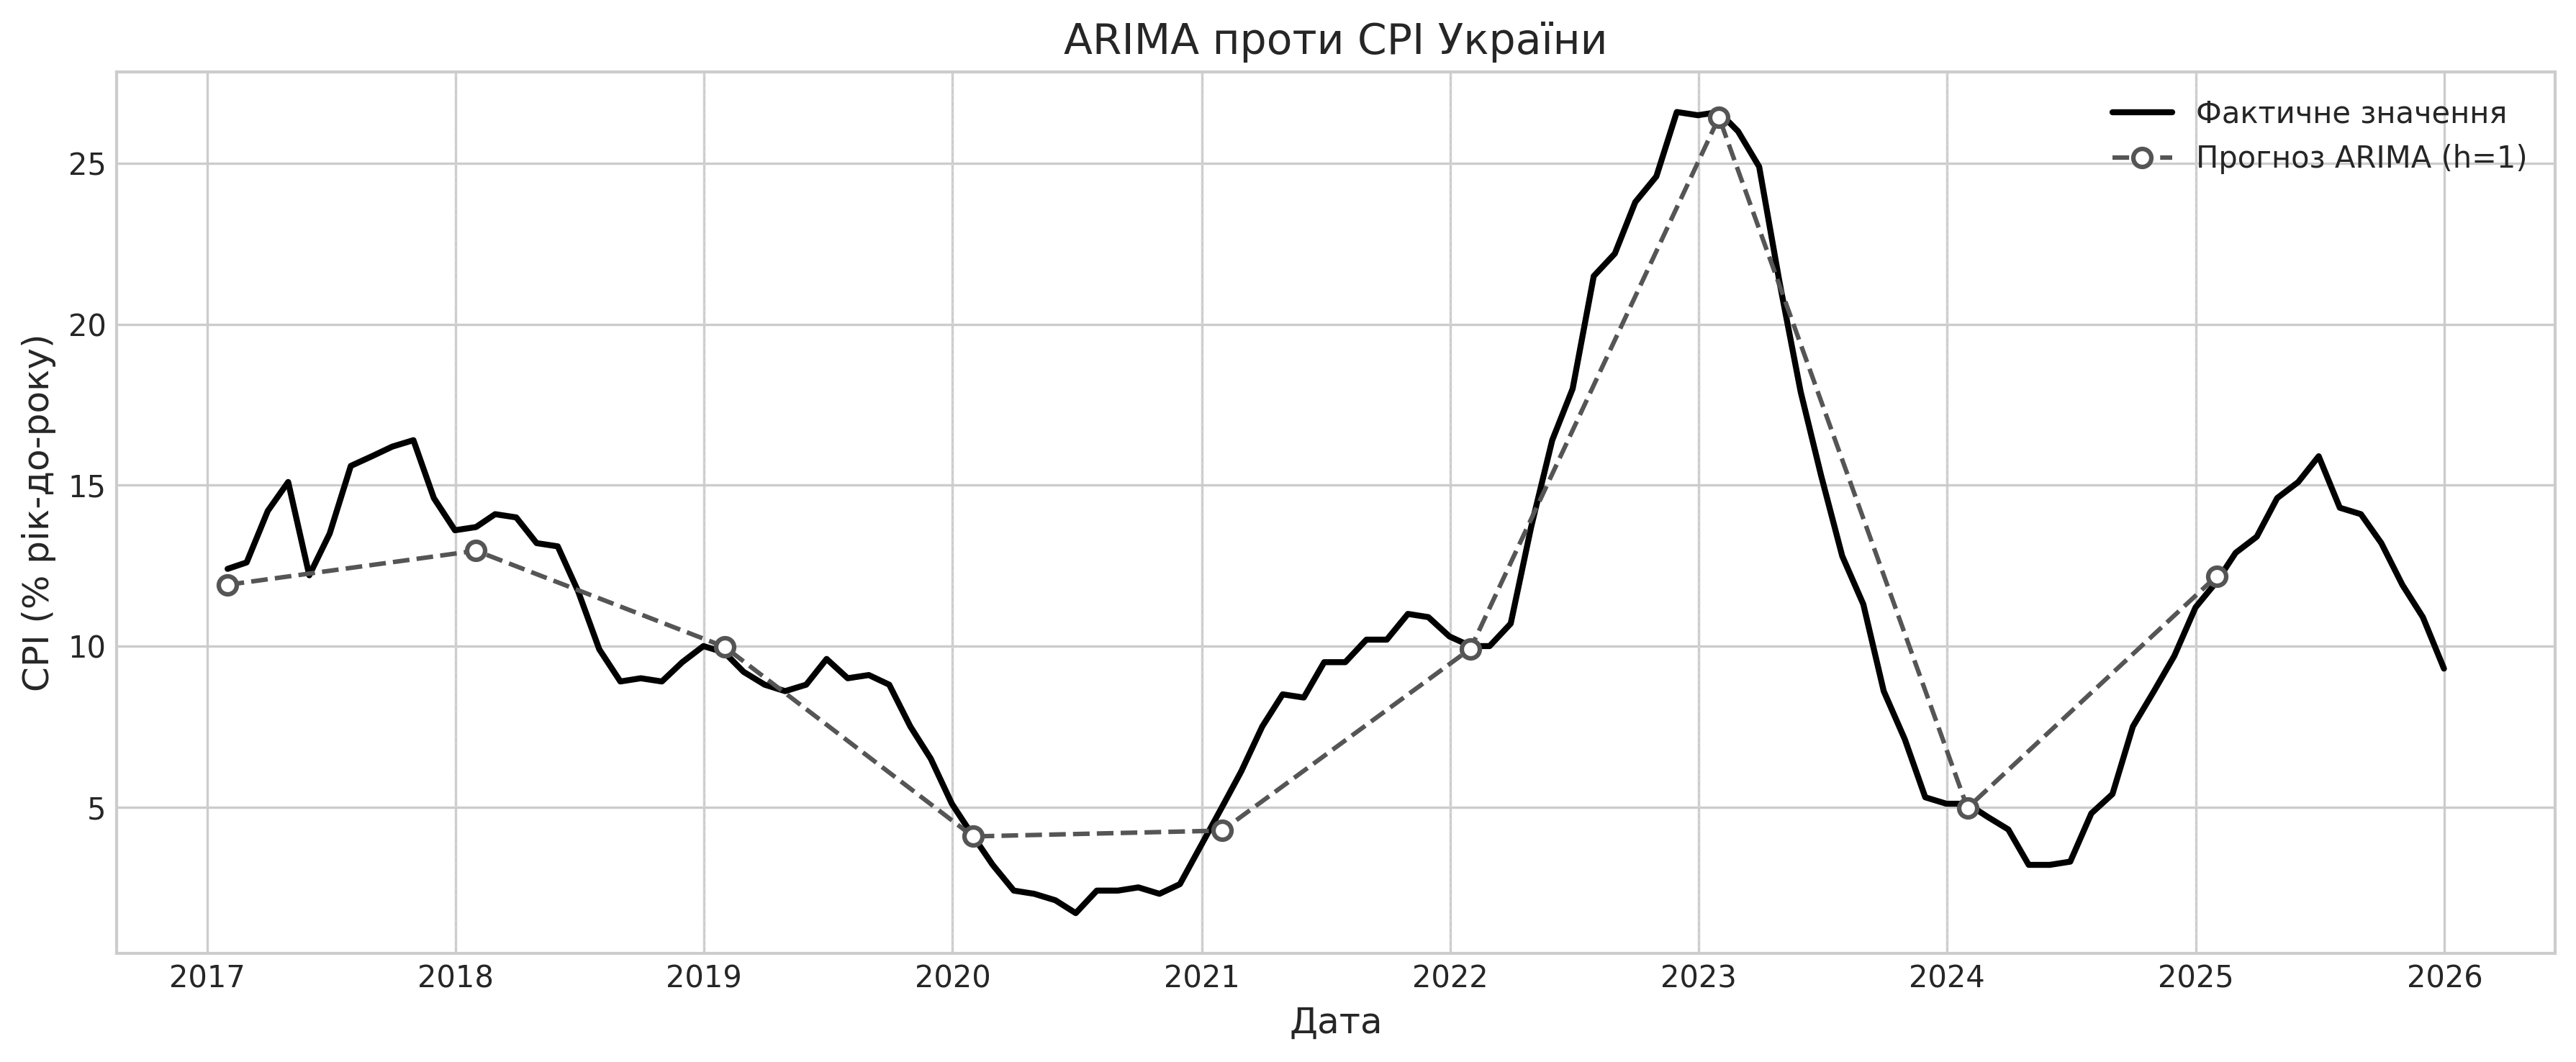
\includegraphics[width=0.95\textwidth]{images/arima_vs_actual_ua.png}
\caption{Прогноз ARIMA проти фактичних значень CPI України (2017--2025)}
\label{fig:arima_vs_actual}
\end{figure}

\subsection{Параметри моделі XGBoost}

Процедура байєсівської оптимізації за допомогою TPE з~150~ітераціями підібрала комбінацію гіперпараметрів XGBoost, наведену в таблиці~3.3.

\begin{table}[h!]
\centering
\begin{tabular}{|l|c|}
\hline
\textbf{Гіперпараметр} & \textbf{Значення} \\
\hline
Швидкість навчання $\eta$ & 0{,}0162 \\
Максимальна глибина дерева $d_{\max}$ & 8 \\
Мінімальна вага дочірнього вузла & 7 \\
Параметр регуляризації за складністю $\gamma$ & 0{,}0626 \\
$L_1$-регуляризація $\alpha$ & 0{,}2797 \\
$L_2$-регуляризація $\lambda$ & 3{,}2458 \\
Частка вибірки \texttt{subsample} & 0{,}9620 \\
Частка ознак \texttt{colsample\_bytree} & 0{,}8414 \\
Оптимальна кількість дерев (рання зупинка) & 13 \\
\hline
\end{tabular}
\caption{Найкращі гіперпараметри XGBoost}
\end{table}

У підібраній конфігурації можна побачити досить великий $L_2$-штраф $\lambda = 3{,}25$ та глибокі дерева $d_{\max} = 8$ з низькою швидкістю навчання $\eta \approx 0{,}016$ які створюють модель, що обережно додає дерева і запобігає перенавчанню. Кожен лист дерева має охоплювати щонайменше 7~спостережень. Після 13 дерев якість валідації погіршується.

\subsection{Порівняння прогнозів моделей}

Далі наведено порівняння RMSE моделей окремо для кожного тестового вікна та зведену середню RMSE. Результати окремих тестів наведені в таблиці~3.4. Жирним шрифтом виділено найкращий результат у тесті серед 5 моделей. Зведені результати наведено в таблиці~3.5.

\begin{table}[!ht]
\centering
\begin{tabular}{|c|c|c|c|c|c|c|}
\hline
\textbf{Вікно} & \textbf{Тест} & \textbf{ARIMA} & \textbf{Гібрид} & \textbf{XGBoost} & \textbf{Вип. бл.} & \textbf{Сез. наїв.} \\
\hline
1 & 2017 & 3{,}1180 & 3{,}8214 & 5{,}8132 & \textbf{2{,}6803} & 14{,}1998 \\
2 & 2018 & 1{,}9888 & \textbf{1{,}8563} & 1{,}8715 & 3{,}0719 & 4{,}4739 \\
3 & 2019 & 2{,}2937 & 2{,}9074 & 2{,}2606 & \textbf{2{,}0704} & 3{,}4902 \\
4 & 2020 & 0{,}6640 & \textbf{0{,}4846} & 14{,}7826 & 2{,}5400 & 5{,}9758 \\
5 & 2021 & 4{,}1798 & 4{,}2370 & \textbf{3{,}7548} & 5{,}4396 & 6{,}6556 \\
6 & 2022 & 11{,}1980 & 9{,}9089 & \textbf{8{,}7925} & 10{,}3695 & 10{,}7261 \\
7 & 2023 & 13{,}5600 & 13{,}5586 & \textbf{11{,}5052} & 13{,}6996 & 14{,}2710 \\
8 & 2024 & 2{,}8419 & 2{,}7115 & 8{,}2238 & \textbf{2{,}7052} & 13{,}4995 \\
9 & 2025 & 1{,}9111 & \textbf{1{,}8673} & 6{,}9478 & 2{,}6369 & 8{,}3783 \\
\hline
\end{tabular}
\caption{Результати моделей за в окремих тестових вікнах}
\end{table}

\begin{table}[h!]
\centering
\begin{tabular}{|l|c|c|}
\hline
\textbf{Модель} & \textbf{Середня RMSE} \\
\hline
Гібрид              & \textbf{4{,}5948} \\
ARIMA               & 4{,}6395 \\
Випадкове блукання  & 5{,}0237 \\
XGBoost             & 7{,}1058 \\
Сезонна наївна      & 9{,}0745 \\
\hline
\end{tabular}
\caption{Середня RMSE моделей}
\end{table}

Найкращу середню якість демонструє гібридна модель зі значенням RMSE = 4{,}5948, однак різниця з чистою ARIMA є мінімальною~-- лише 0{,}1048 , або близько 0{,}96\% від базового рівня. Хоча гібрид має кращий результат за ARIMA у 6 з 9 тестів, а чиста ARIMA жодного разу не дала найкращого прогнозу серед усіх 5 моделей. Окремий XGBoost має найкращий результат у трьох тестах, проте середня RMSE значно гірша за гібридну модель та просту ARIMA, навіть випадкові блукання в середньому дають кращий результат. Сезонний наївний прогноз є зовсім неконкурентоспроможним.

Окремо було проведено горизонтний аналіз на вибірці за 2025 рік для 1, 3, 6 та 12 місяців по кожній моделі. Зіставлення результатів на чотирьох горизонтах прогнозування відображено на рисунку~3.2, значення помилок наведені в таблиці 3.6.

\begin{figure}[h!]
\centering
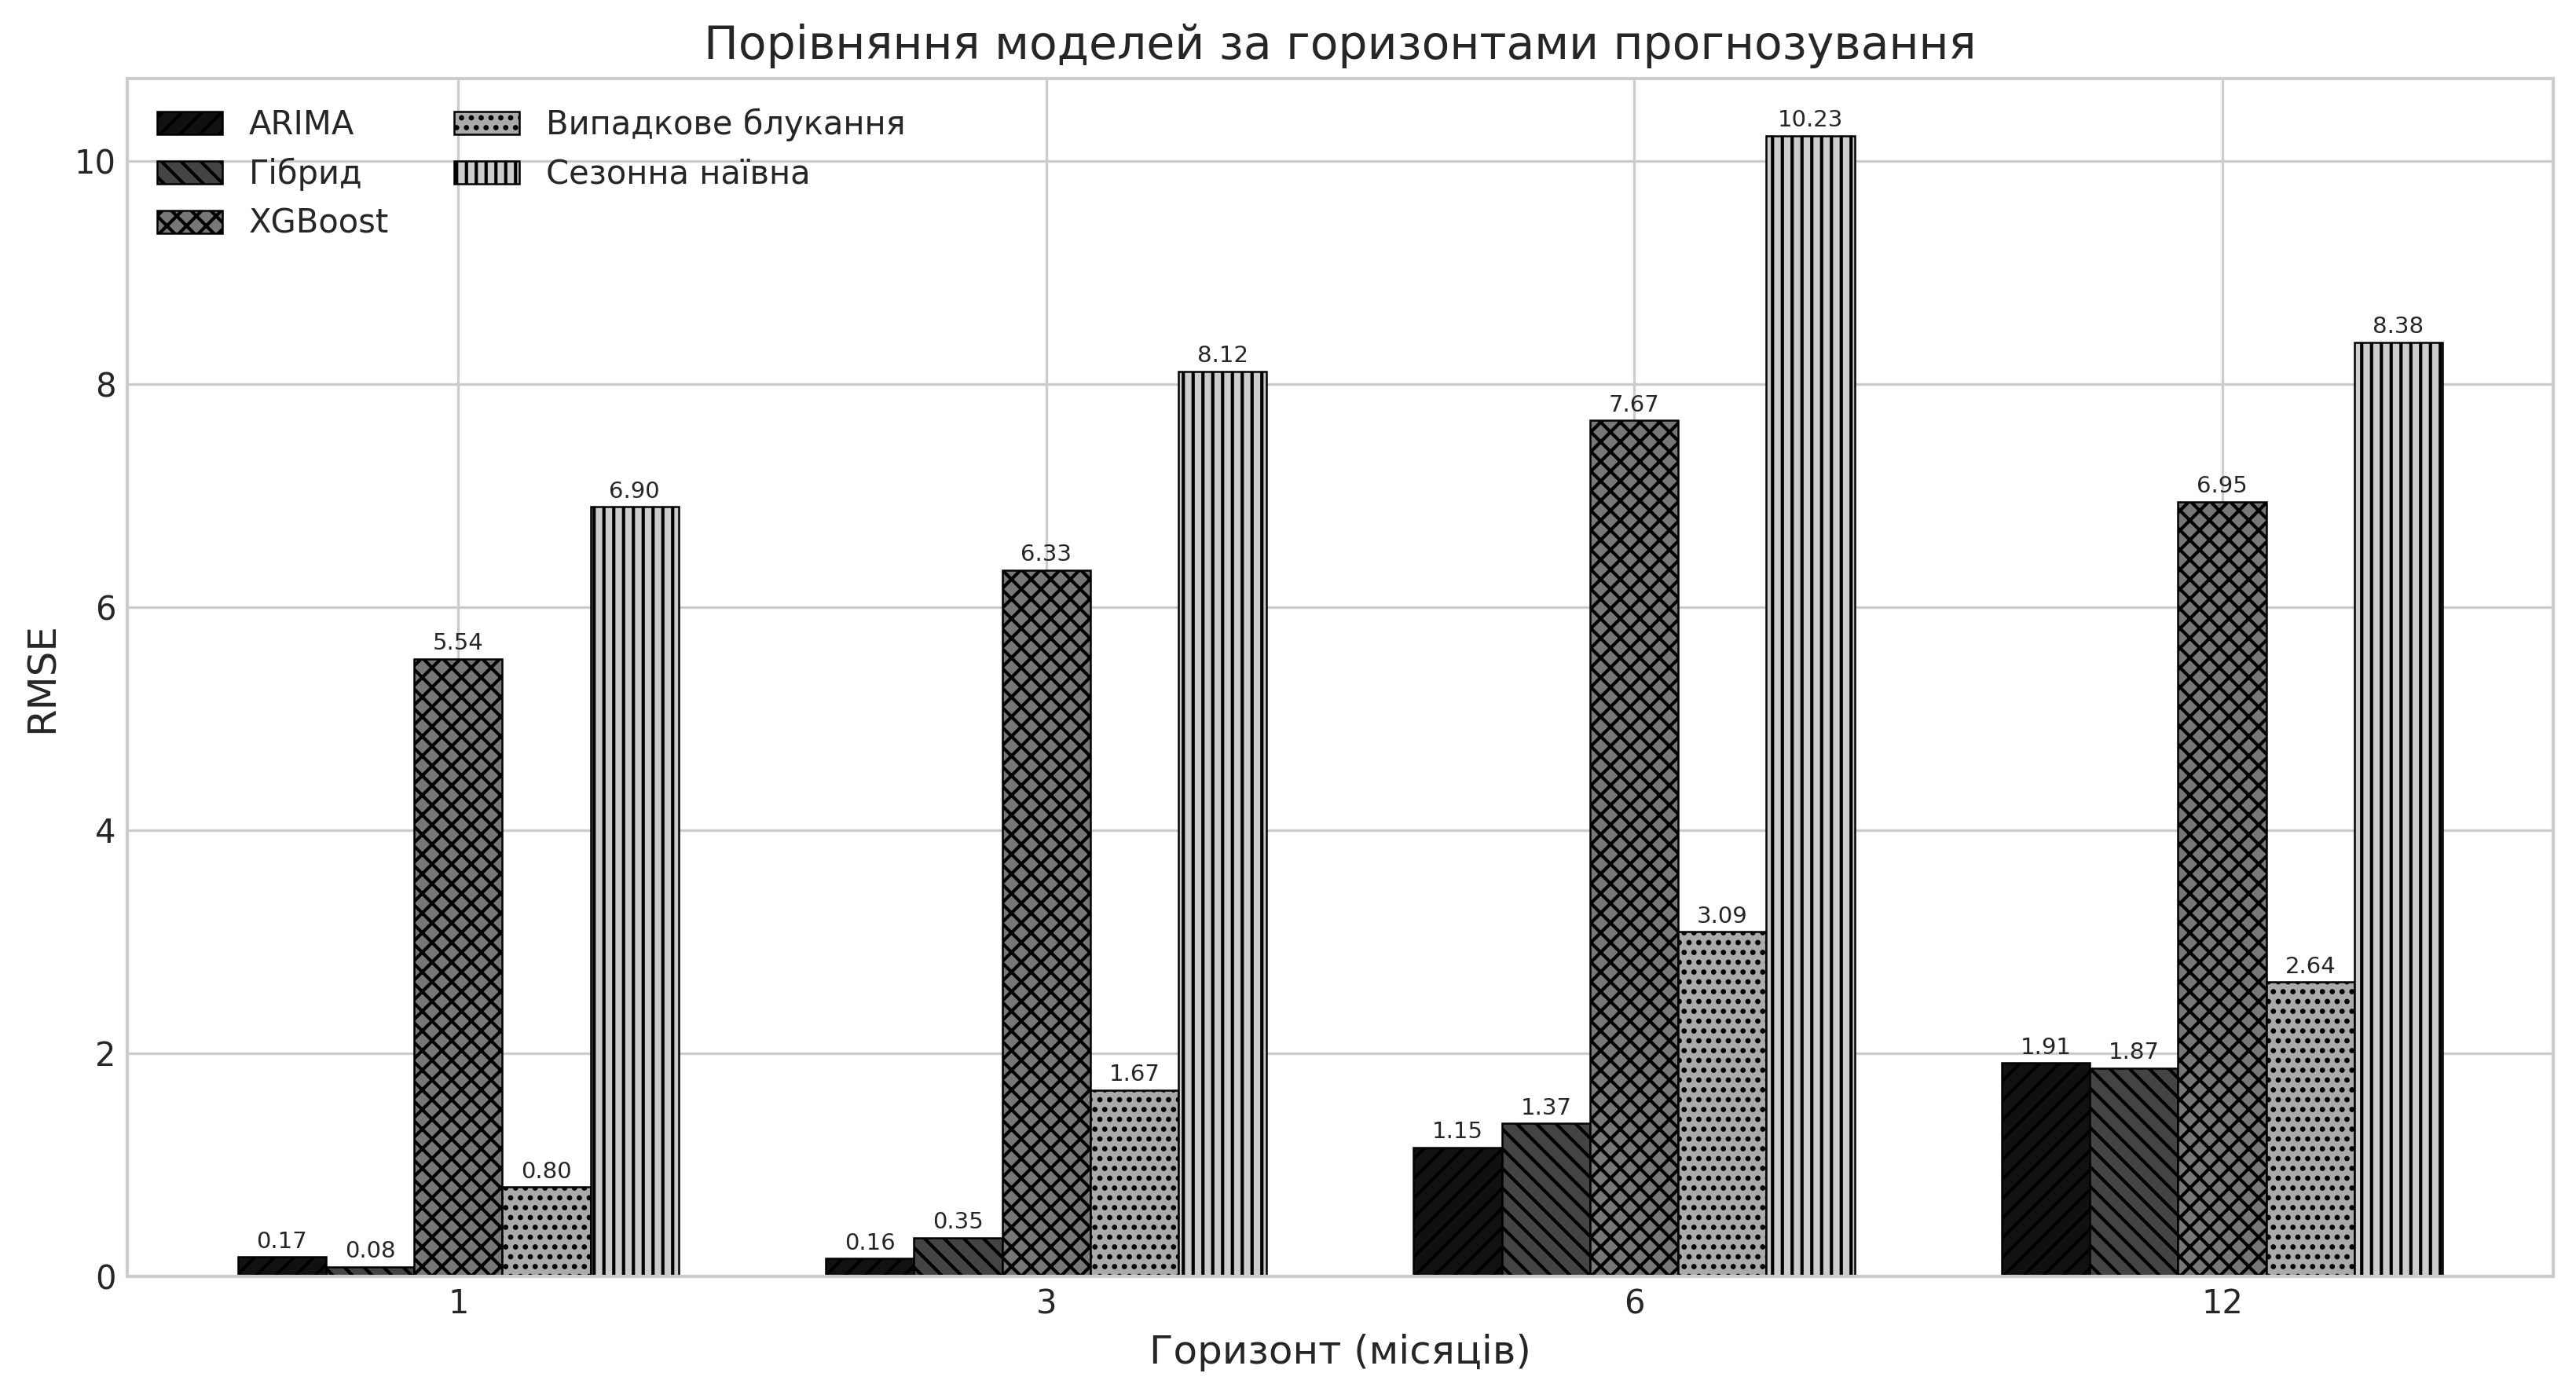
\includegraphics[width=0.95\textwidth]{images/rmse_by_model_horizon.png}
\caption{Порівняння моделей за горизонтами прогнозування (2025~р.)}
\label{fig:rmse_bars}
\end{figure}

\begin{table}[h!]
\centering
\begin{tabular}{|c|c|c|c|c|c|}
\hline
\textbf{Гор-нт} & \textbf{ARIMA} & \textbf{Гібрид} & \textbf{XGBoost} & \textbf{Вип. бл.} & \textbf{Сез. наїв.} \\
\hline
$h=1$  & 0{,}1729 & \textbf{0{,}0844} & 5{,}5390 & 0{,}8000 & 6{,}9000 \\
$h=3$  & \textbf{0{,}1570} & 0{,}3458 & 6{,}3322 & 1{,}6703 & 8{,}1171 \\
$h=6$  & \textbf{1{,}1547} & 1{,}3694 & 7{,}6742 & 3{,}0884 & 10{,}2306 \\
$h=12$ & 1{,}9111 & \textbf{1{,}8673} & 6{,}9478 & 2{,}6369 & 8{,}3783 \\
\hline
\end{tabular}
\caption{Порівняння моделей за горизонтами прогнозування (2025~р.)}
\end{table}

На рисунку 3.3 наведена залежність помилки від горизонту прогнозування.

\begin{figure}[h!]
\centering

\includegraphics[width=0.95\textwidth]{images/rmse_vs_horizon.png}
\caption{Залежність якості прогнозу від горизонту прогнозування}
\label{fig:rmse_lines}
\end{figure}

Можна побачити, що гібрид показує найкращий результат на найкоротшому горизонті $h=1$ (RMSE = 0{,}0844 проти 0{,}1729 для ARIMA, в два рази краще) і на найдовшому $h=12$ (1{,}87 проти 1{,}91 для ARIMA). На середніх горизонтах $h=3$ і $h=6$ перевагу має чиста ARIMA. Чистий XGBoost показав найгірший результат на всіх горизонтах серед нетривіальних моделей, що підтверджує необхідність компонента ARIMA для вловлення базової інерційної структури ряду, яка дає найбільший внесок у прогноз.

Загалом за результатами можна побачити високу варіативність результатів між вікнами. Стандартне відхилення дорівнює близько 4~ для всіх моделей. Це демонструє складність прогнозування інфляції України, адже тестовий період 2017--2025~рр. охоплює періоди різної природи~-- стабільний 2018--2019~рр., COVID 2020~р., післяковідну інфляцію 2021~р., війна 2022~р., поступову дезінфляцію 2023~р. Жодна модель не демонструє стабільно низького RMSE: у 2022~р. гібрид показав RMSE = 9{,}91, тоді як у спокійному 2020~р.~-- лише 0{,}48.

Цінність гібриду проявляється асиметрично залежно від режиму інфляції.
У кризові роки —- зокрема 2022 —- гібрид знизив RMSE з 11{,}20 до 9{,}91
(-11{,}5\%), оскільки залишки ARIMA містили стійкий нелінійний сигнал,
пов'язаний із геополітичними та валютними шоками, який XGBoost зміг
ідентифікувати через ознаки GPR та курсу EUR.

Натомість у стабільні роки XGBoost є надлишковим:
у 2017~р. Hybrid поступився ARIMA (3{,}82 проти 3{,}12). Причиною є те, що в умовах передбачуваної
інфляції залишки ARIMA наближаються до білого шуму, тобто не містять
реального нелінійного сигналу, який можна було б вловити. XGBoost, проте,
навчається на цих залишках і виявляє уявні кореляції в тренувальній вибірці, що призводить до систематичного внесення шуму у кінцевий прогноз. Це пояснює, чому середнє покращення гібриду над чистим ARIMA є мінімальним -- лише 2{,}3\% -— попри перевагу в кризових вікнах.


Для статистичної перевірки значущості відмінностей між прогнозами застосовано тест Діболда-Маріано за формулою~\eqref{eq:dm_test} на всіх тестових вікнах. Як тестову статистику використано різницю середньоквадратичних похибок між парами моделей: $d_w = \text{RMSE}^2_{\text{hybrid},w} - \text{RMSE}^2_{\text{bench},w}$. Результати наведено в таблиці~3.7.

\begin{table}[h!]
\centering
\begin{tabular}{|l|c|c|l|}
\hline
\textbf{Порівняння} & \textbf{DM-статистика} & \textbf{$p$-значення} & \textbf{Висновок} \\
\hline
Гібрид vs ARIMA        & $-0{,}71$ & $0{,}499$  & Не значущо \\
Гібрид vs XGBoost      & $-1{,}12$ & $0{,}295$  & Не значущо \\
Гібрид vs Вип.\ блук.  & $-1{,}56$ & $0{,}157$  & Не значущо \\
Гібрид vs Сез.\ наїва  & $-2{,}59$ & $0{,}032$  & Значущо \\
\hline
\end{tabular}
\caption{Результати тесту Діболда-Маріано}
\label{tab:dm_test}
\end{table}

Від'ємна DM-статистика означає, що гібрид має меншу квадратичну помилку. Хоча жодна з відмінностей не досягає статистичної значущості на рівні 1\%. Проте це є очікуваним для невеликої кількості спостережень, адже тест Діболда-Маріано має низьку ефективність при малій вибірці. Лише перевага над сезонною наївною підтверджується на рівні 5\%.

\subsection{Інтерпретація моделі SHAP}

Для розуміння внеску окремих чинників гібридної моделі обчислено значення SHAP для всіх 14~предикторів. Глобальну важливість ознак, обчислену як усереднені абсолютні значення SHAP за формулою~\eqref{eq:shap_global}, наведено в таблиці~3.8 (перші 10 найважливіших) та візуалізовано на рисунку~3.4.


\begin{table}[h!]
\centering
\begin{tabular}{|c|l|c|c|}
\hline
\textbf{№} & \textbf{Ознака} & \textbf{Середнє $|\text{SHAP}|$} & \textbf{Частка} \\
\hline
1  & Курс EUR                       & 0{,}4731 & 36{,}0\% \\
2  & Курс USD                       & 0{,}1921 & 14{,}6\% \\
3  & Грошова маса M3                & 0{,}1668 & 12{,}7\% \\
4  & Індекс геополітичного ризику   & 0{,}1293 &  9{,}8\% \\
5  & Індекс цін металів             & 0{,}0609 &  4{,}6\% \\
6  & Реальний ефективний курс       & 0{,}0532 &  4{,}0\% \\
7  & Індекс VIX                     & 0{,}0447 &  3{,}4\% \\
8  & Промвиробництво                & 0{,}0445 &  3{,}4\% \\
9  & Ключова ставка                 & 0{,}0257 &  2{,}0\% \\
10 & ВВП                            & 0{,}0231 &  1{,}8\% \\
\hline
\end{tabular}
\caption{10 найбільш значущих ознак за SHAP (частки від суми всіх ознак)}
\end{table}

\begin{figure}[h!]
\centering
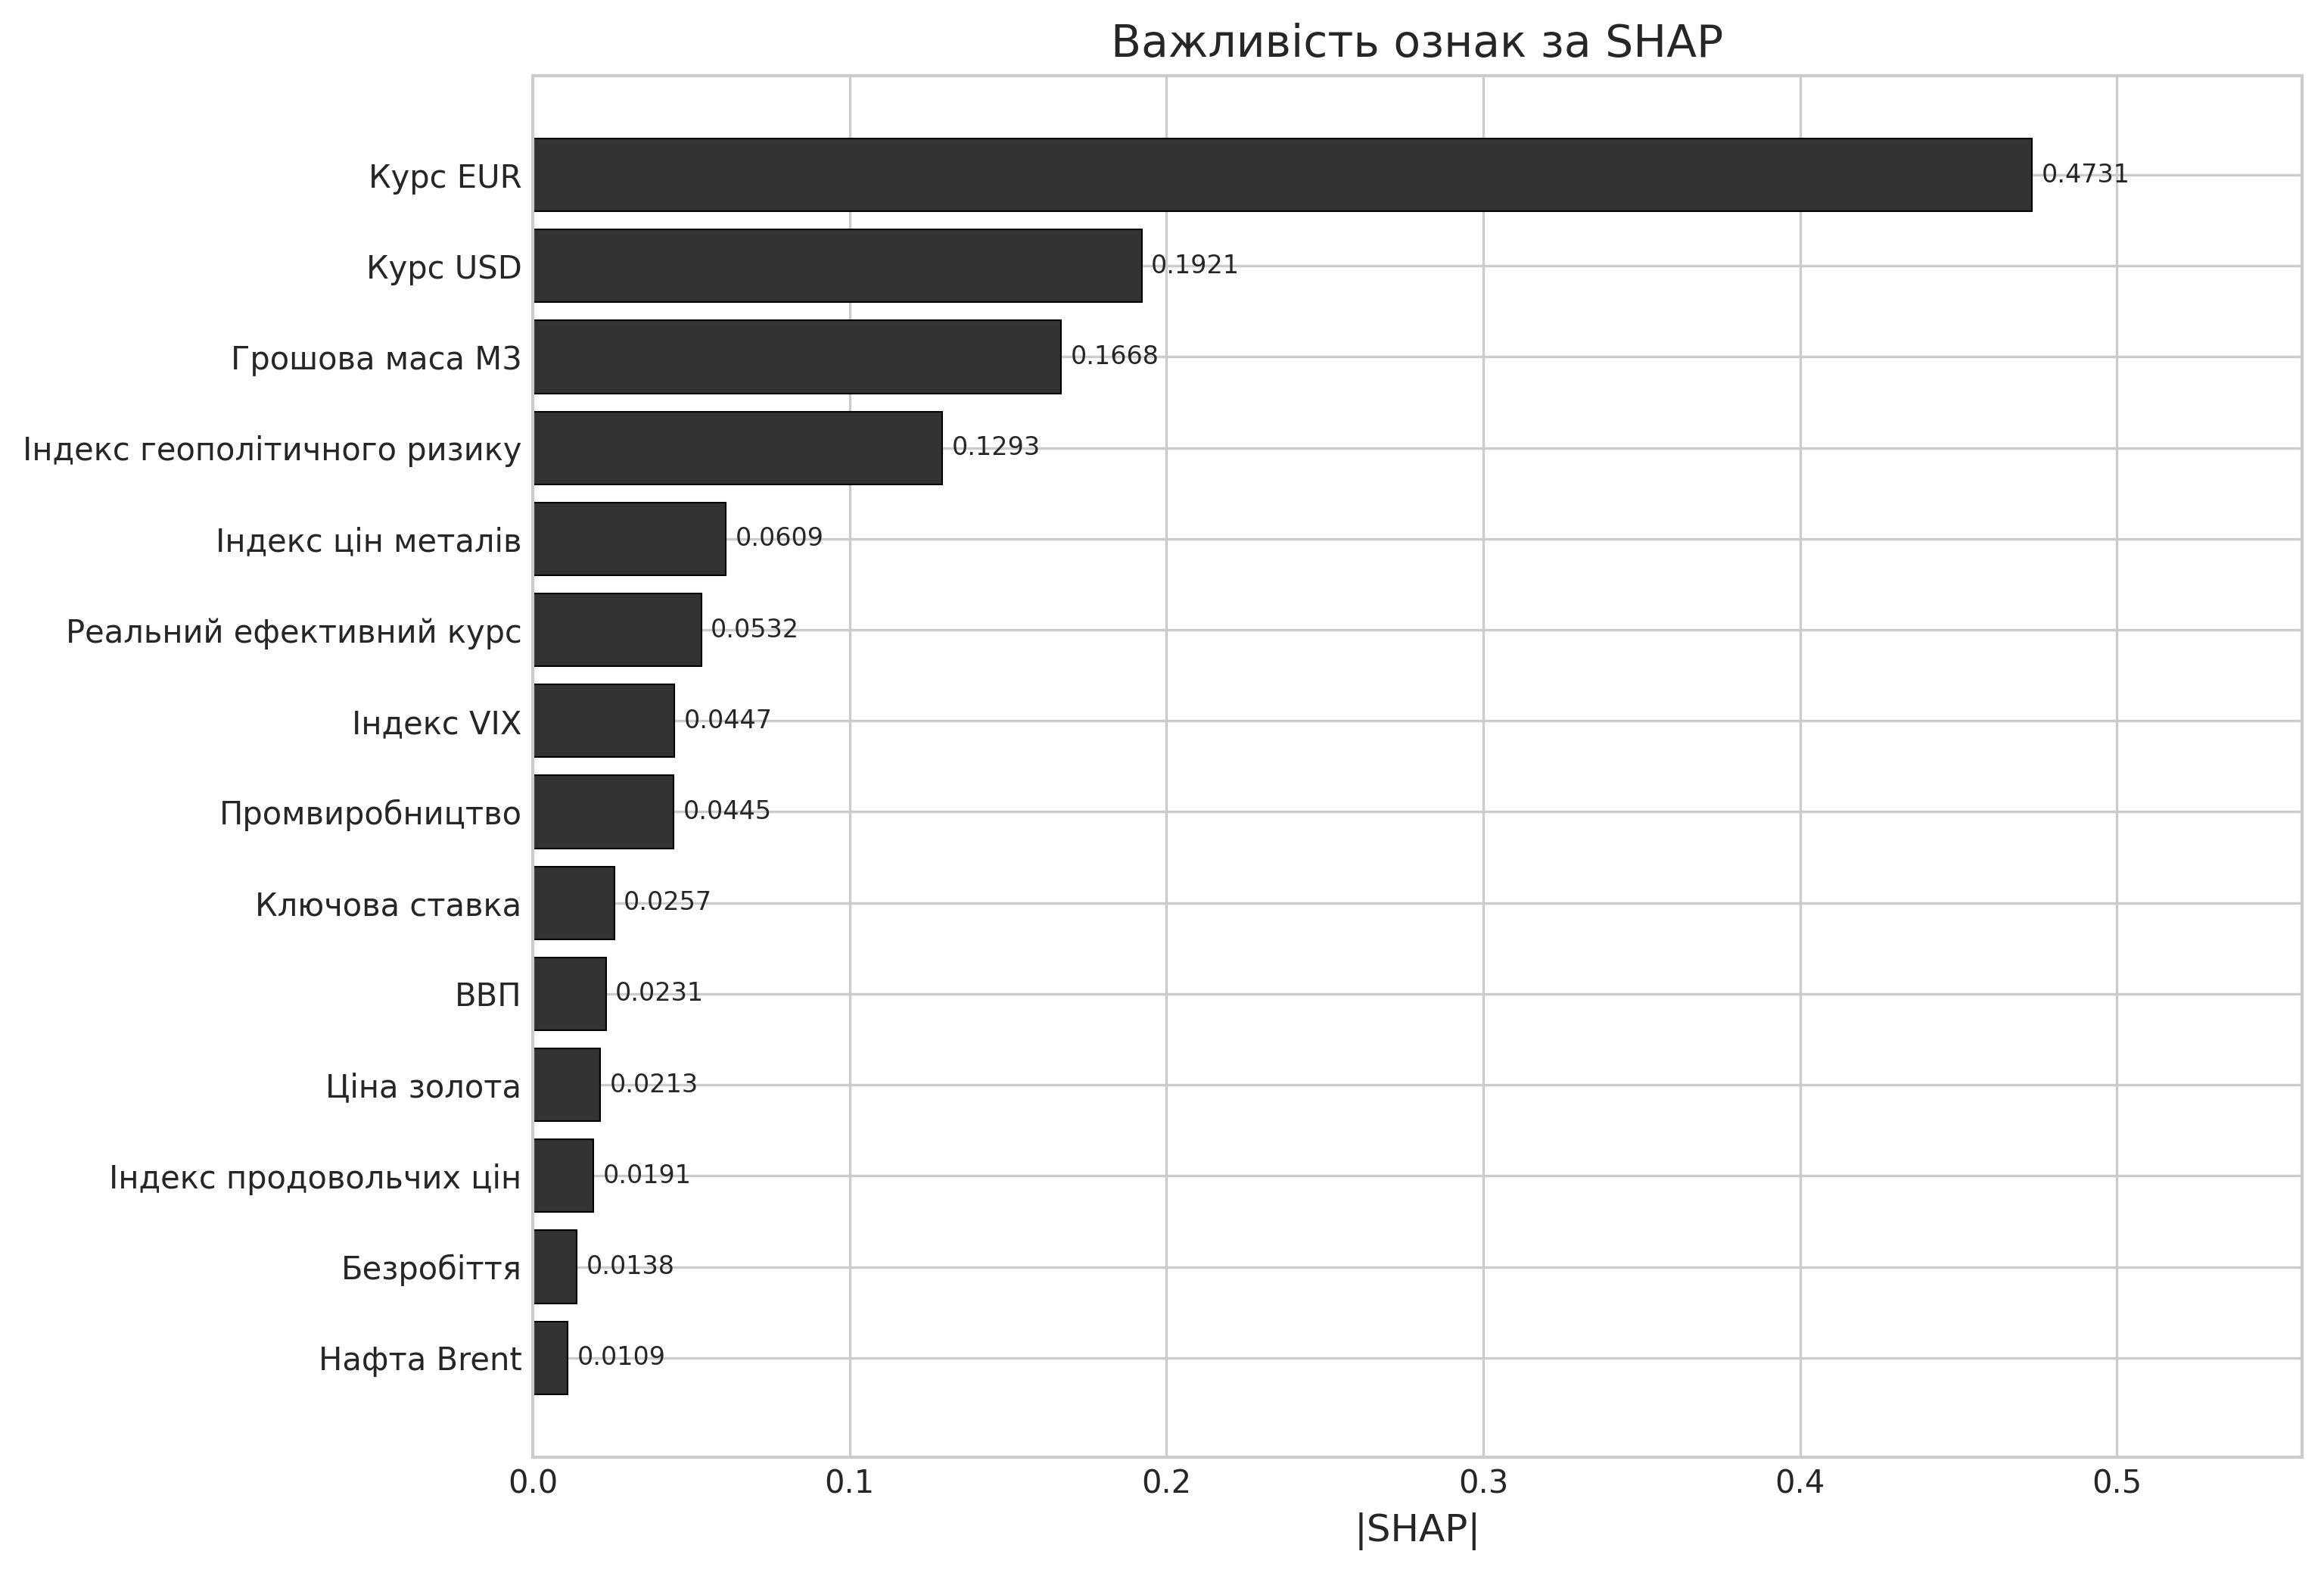
\includegraphics[width=0.95\textwidth]{images/shap_global_importance.png}
\caption{Глобальна важливість ознак за SHAP}
\label{fig:shap_global}
\end{figure}

Найвпливовішими ознаками є курси гривні до долара США та євро. Далі йде грошова маса M3, і разом ці три ознаки забезпечують 63{,}3\% сукупного внеску компонентів у прогноз XGBoost. Аналіз SHAP виконано на тестовій вибірці виключно для України і має вагу не для всіх економік, адже в країнах Балтії евро є національною валютою, і відповідно значення показника курсу є константою, а отже і не має жодного впливу на прогноз інфляції. Проте для економік подібних Україні із плаваючим курсом валют важливість є обгрунтованою. Висока важливість курсів євро та долару США відображає динаміку гривні для якої девальвація до інших валют транслюється в зростання цін на імпорт. Це підтверджує твердження з підрозділу~1.1.2 про визначальну роль валютного каналу передачі в українській малій відкритій економіці згідно з формулою~\eqref{eq:pass_through}.


Також серед найвпливовіших чинників є зовнішні показники, як індекс геополітичного ризику, VIX індекс та індекс цін металів. Це демонструє, що модель враховує зовнішні чинники які дійсно мають вплив на інфляцію. Отже модель враховує не ізольовану економіку, а й вплив зовнішніх факторів. Окрім зовнішніх показників, є й очевидні внутрішні, як ВВП, ключова ставка, РЕОК та індекс промислового виробництва. Отже загалому можна сказати, що набір є логічним та підтверджується на практиці, адже як було зазначено круси валют сильно впливають на CPI, зовнішні чиники в свою чергу в певній мірі демонструють тенденції в імпорті та експорті, ВВП безпосередньо реагує на інфляцію а ключова ставка є інструментом для її стримування.

Розподіл SHAP-значень для кожної ознаки на тестовій вибірці подано на рисунку~3.5, що дозволяє побачити не лише силу впливу ознаки, а й напрям цього впливу та залежність від конкретного значення ознаки.

\begin{figure}[h!]
\centering
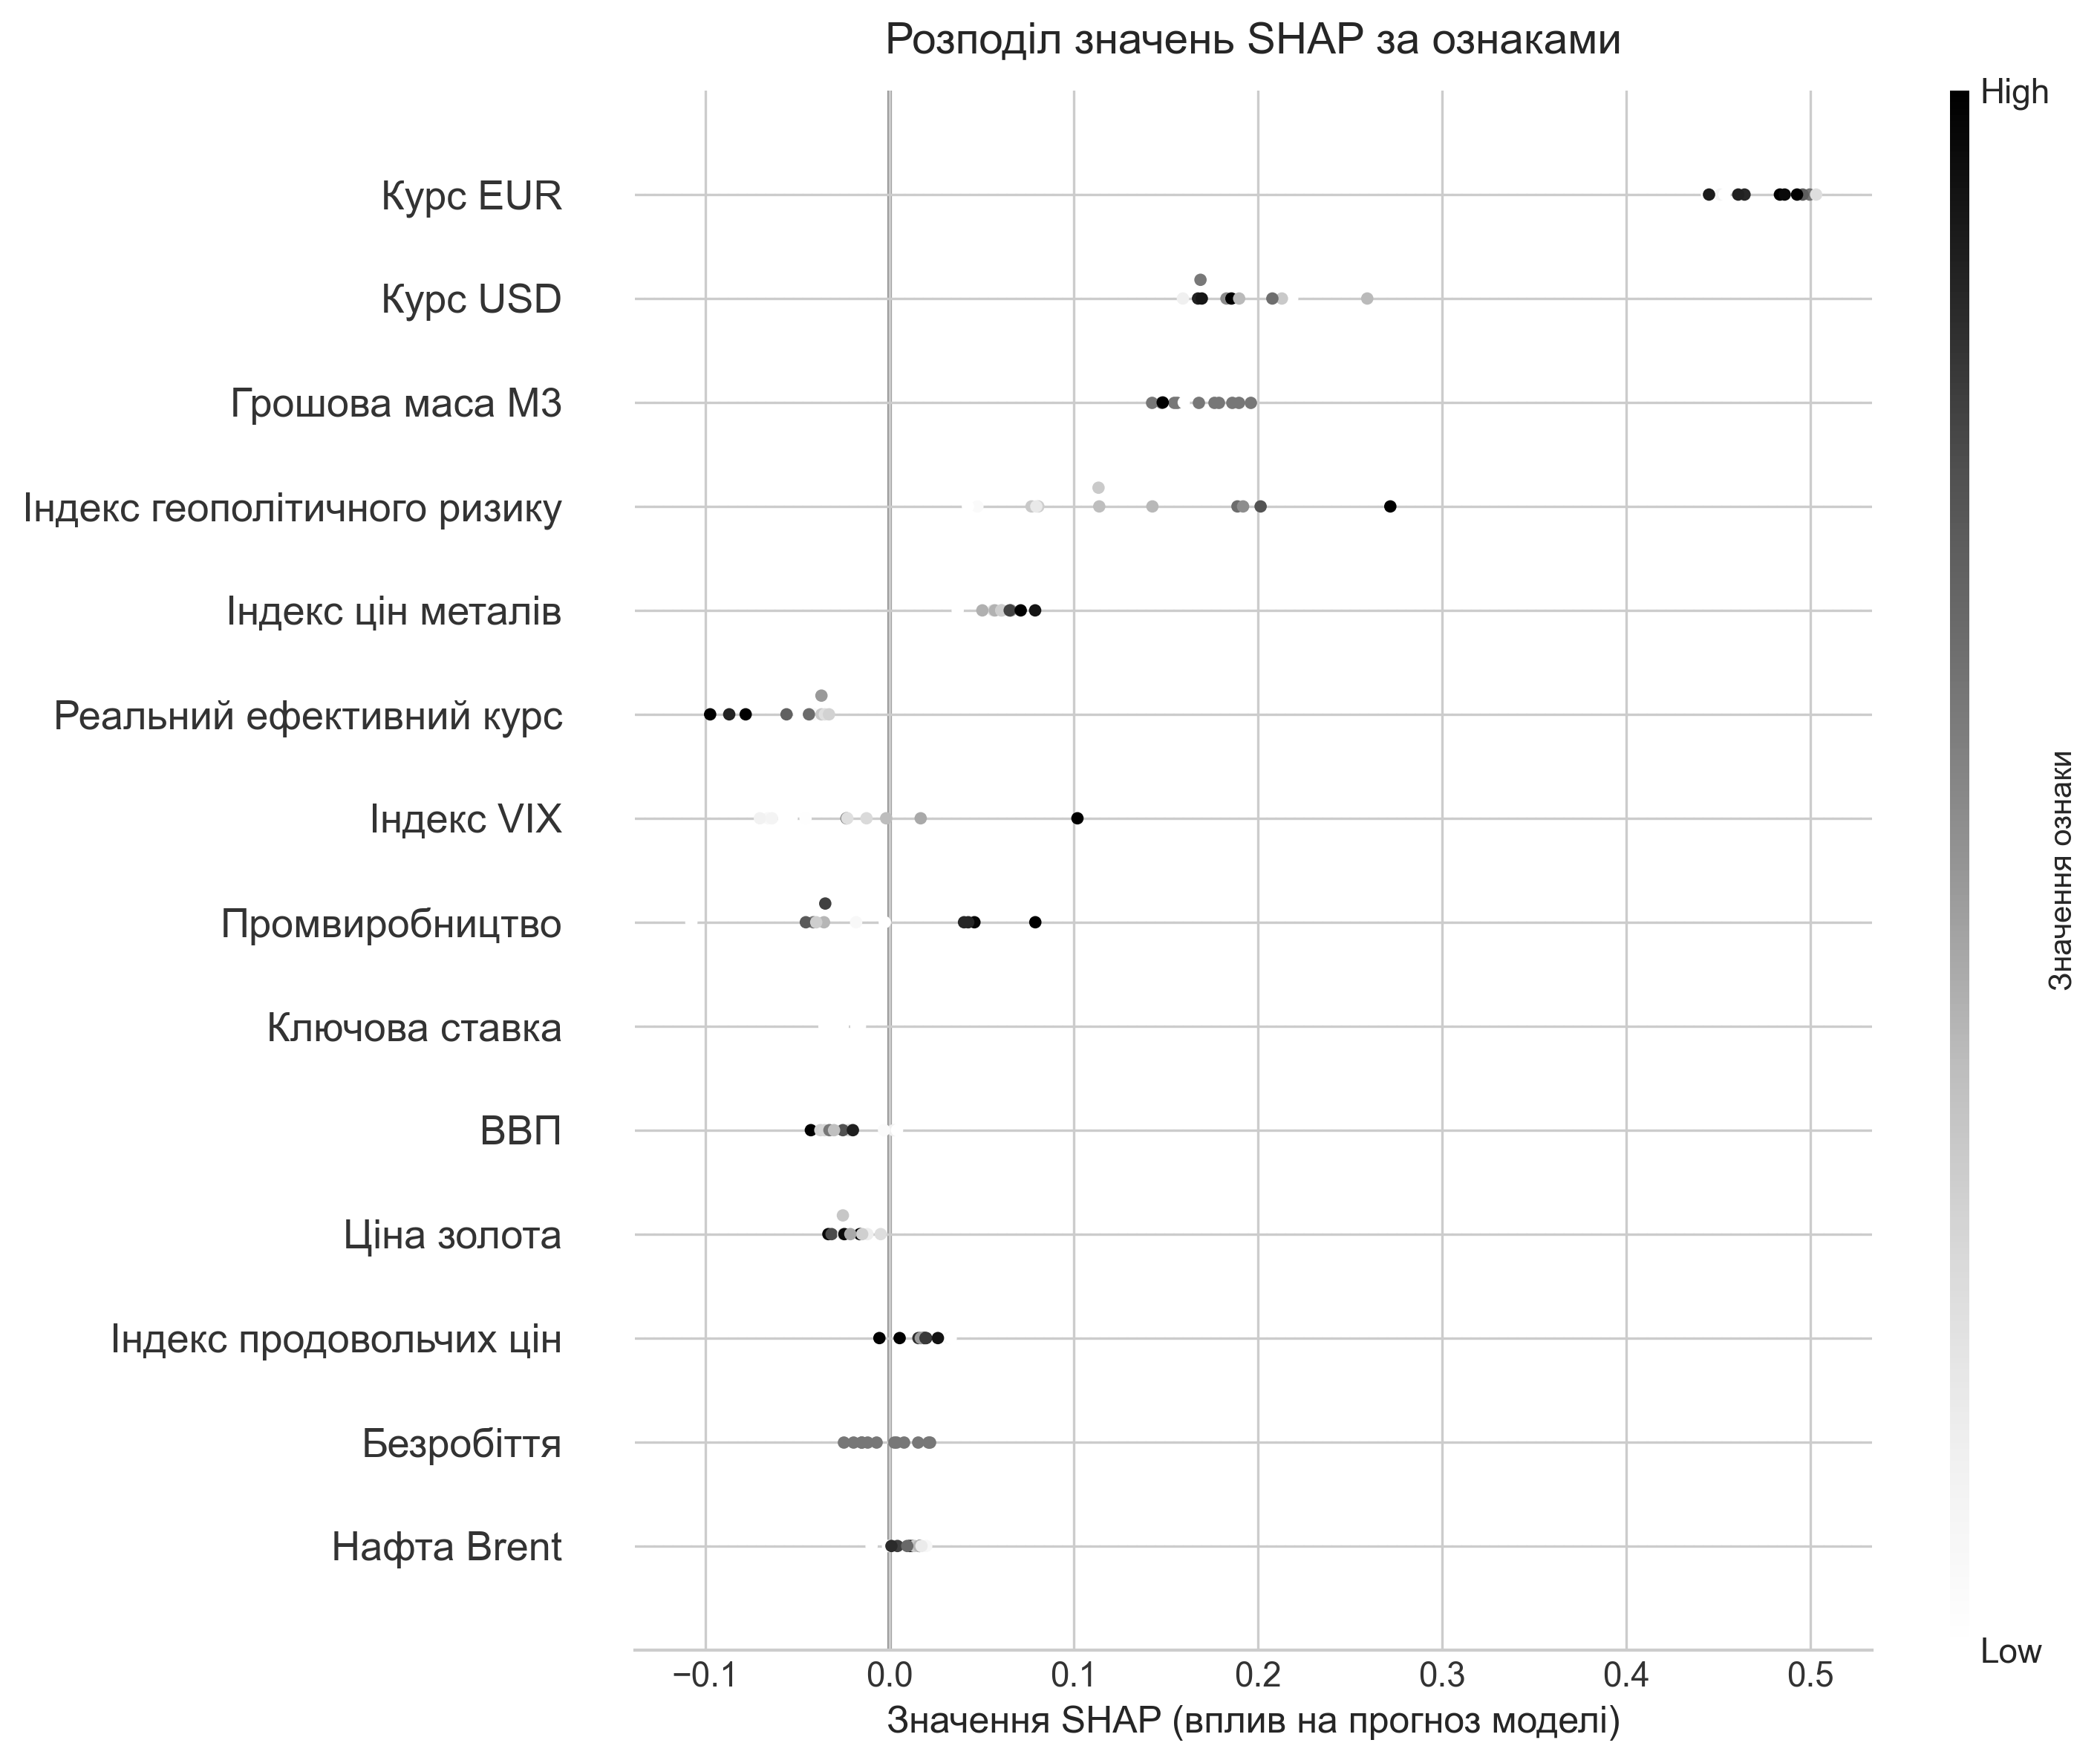
\includegraphics[width=0.95\textwidth]{images/shap_beeswarm.png}
\caption{Розподіл SHAP-значень за ознаками}
\label{fig:shap_beeswarm}
\end{figure}

Розподіл відображає поведінку моделі в одному конкретному тестовому вікні (2025~р.), а не стійку середню картину по всіх вікнах крос-валідації. Для трьох провідних предикторів спостерігається очікувана структура: високі значення курсу пов'язані з позитивними SHAP-значеннями, тобто збільшують прогнозовану інфляцію, а низькі значення -- навпаки.

\chapconclude{3}

У цьому розділі описано процес підготовки даних. Було обґрунтовано вибір показників, описано джерела їх збору та необхідні дії для підготовки їх до використання. Також зазначено підходи до заповнення наявних пропусків даних.

Було описано програмну реалізацію експерименту, а саме моделей, підбор параметрів, розбиття на тренувальні та тестові вибірки. Описано принципи оцінювання та бенчмарки.

Наприкінці зазначено отримані результати та проведено SHAP-аналіз прогнозу для візуалізації найвпливовіших показників. За результатами в середньому гібридна модель показала найкращі результати.

\newpage
\thispagestyle{plain}
\doublespacing
\setfontsize{14}
\addcontentsline{toc}{chapter}{Висновки}

\begin{center}
    {\bfseries\Large\MakeUppercase{Висновки}}
\end{center}

\vspace{14pt}

Одним із перших завдань роботи було провести дослідження інфляції в цілому та інфляції України зокрема, а також методів її прогнозування й інтерпретації прогнозів. На початку було обґрунтовано проблему інфляції у світі. На основі проаналізованих джерел зазначено бажаний рівень інфляції та інструменти для його досягнення, чинники, що впливають на інфляцію, а також методи прогнозування та інтерпретації прогнозів. На основі вивченого матеріалу було обрано ARIMA, XGBoost та SHAP моделі для проведення експерименту.

На основі обраних моделей було описано гібридну архітектуру моделі для врахування інерції цін за допомогою ARIMA, розрахунку впливу нелінійних чинників за допомогою XGBoost та інтерпретацію прогнозу за допомогою SHAP. Для порівняння моделей та визначення їхньої ефективності було обрано бенчмарки у вигляді окремих моделей ARIMA та XGBoost, а також примітивних моделей випадкового блукання та наївної сезонної моделі.

Для проведення експерименту було зібрано набір даних із внутрішніх показників України та зовнішніх економічних показників. Через нестачу українських даних було залучено дані Литви та Латвії для тренування моделі через подібність їхніх економік. За допомогою зібраного набору даних та описаного алгоритму було проведено експеримент. За результатами 9-ти тестів на різних часових проміжках гібридна модель в середньому показала себе найкраще, на 0{,}96\% краще ARIMA, 9{,}33\% краще випадкових блукань, 54{,}64\% краще XGBoost та на 97{,}49\% краще сезонної наївної моделі. Хоча аналіз прогнозування на 1, 3, 6 та 12 місяців дав неоднозначний результат і гібридна модель перевершила всі інші лише на горизонті 1 та 12 місяців, вона значно краще показує себе при прогнозуванні кризових років, де стандартна ARIMA не дає якісного результату через неспроможність враховувати нелінійні показники. Тест Діболда-Маріано не виявив статистично значущої різниці між гібридом та ARIMA ($p=0{,}499$), що є закономірним за невеликої вибірки. Єдине значуще підтвердження отримано порівняно із сезонною наївною ($p=0{,}032$).


За результатами експерименту можна виокремити декілька можливих майбутніх покращень для цього дослідження. Перш за все -- мінімізувати негативний вплив на результат, спричинений нестачею даних. Варто розширити набір економічних показників для широшого аналізу та зібрати більше спостережень. Можливим варіантом є застосування моделі до економік із довшою історією та відкритішими наборами даних. Аналіз по вікнах виявив виражену залежність внеску XGBoost від періоду: у кризових вікнах (2022: -11{,}5\%, 2020: -27\%) гібрид суттєво переважає ARIMA, тоді як у стабільних вікнах (2017: +22{,}5\%) XGBoost додає шум замість сигналу, бо залишки ARIMA є близькими до білого шуму і реальних нелінійних залежностей для навчання немає. Для подалання надлишковості XGBoost у стабільні періоди можна реалізувати є зважену модель з адаптивними коефіцієнтами, де вага XGBoost-компоненти знижується автоматично у стабільних умовах -- наприклад через навчання на додаткових ознаках періоду (волатильність CPI, GPR тощо).


% ============================================================
%  Список використаних джерел
% ============================================================
\newpage
\addcontentsline{toc}{chapter}{Список використаних джерел}
\begin{center}
    {\bfseries\Large\MakeUppercase{Список використаних джерел}}
\end{center}

\vspace{12pt}

\begin{enumerate}[label={[\arabic*]}, leftmargin=0pt, itemindent=0pt, labelindent=0pt]

\item Measuring inflation and consumer prices / European Central Bank. --- URL: \url{https://www.ecb.europa.eu/stats/macroeconomic_and_sectoral/hicp/html/index.en.html} (дата звернення: 15.02.2026).

\item Кириленко В.~В. Макроекономіка: курс лекцій / за ред. В.~В.~Кириленка. --- Тернопіль~: Економічна думка, 2008. --- 252~с. --- URL: \url{https://dspace.wunu.edu.ua/handle/316497/28895} (дата звернення: 05.03.2026).

\item Lagarde C. Monetary policy in a high inflation environment: commitment and clarity : speech at the 5th annual conference organised by the European Fiscal Board, Frankfurt, 4 November 2022 / C.~Lagarde // European Central Bank. --- URL: \url{https://www.ecb.europa.eu/press/key/date/2022/html/ecb.sp221104_1~8be9a4f4c1.en.html} (дата звернення: 15.02.2026).

\item Brunnermeier M.~K. The Debt-Inflation Channel of the German Hyperinflation / M.~K.~Brunnermeier, S.~Correia, S.~Luck, E.~Verner, T.~Zimmermann // MPRA Paper. --- 2023. --- №~119195. --- URL: \url{https://mpra.ub.uni-muenchen.de/119195/1/MPRA_paper_119195.pdf} (дата звернення: 15.02.2026).

\item VoxUkraine. Inflation in Ukraine: Past, Present and Future. --- URL: \url{https://voxukraine.org/en/inflation-in-ukraine-past-present-and-future} (дата звернення: 17.02.2026).

\item Banaian K. The Ukrainian Economy since Independence / K.~Banaian. --- Cheltenham~: Edward Elgar Publishing, 1999. --- 144~с. --- (Studies of Communism in Transition). --- URL: \url{https://www.e-elgar.com/shop/usd/the-ukrainian-economy-since-independence-9781858989907.html} (дата звернення: 17.02.2026).

\item Faryna O. Nonlinear Exchange Rate Pass-Through to Domestic Prices in Ukraine / O.~Faryna // Visnyk of the National Bank of Ukraine. --- 2016. --- №~236. --- С.~30--42. --- DOI:~10.26531/vnbu2016.236.030. --- URL: \url{https://doi.org/10.26531/vnbu2016.236.030}.

\item Rakic D. Two years of war: The state of the Ukrainian economy in ten charts : Briefing PE~747.858 / D.~Rakic // Economic Governance and EMU Scrutiny Unit, European Parliament. --- 2024. --- URL: \url{https://www.europarl.europa.eu/RegData/etudes/BRIE/2024/747858/IPOL_BRI(2024)747858_EN.pdf} (дата звернення: 17.02.2026).

\item Zholud O. The Effectiveness of the Monetary Transmission Mechanism in Ukraine since the Transition to Inflation Targeting / O.~Zholud, V.~Lepushynskyi, S.~Nikolaychuk // Visnyk of the National Bank of Ukraine. --- 2019. --- №~247. --- С.~19--37. --- DOI:~10.26531/vnbu2019.247.02. --- URL: \url{https://doi.org/10.26531/vnbu2019.247.02}.

\item Kravchuk R.~S. Budget Deficits, Hyperinflation and Stabilization in Ukraine, 1991-96 / R.~S.~Kravchuk // Public Budgeting~\& Finance. --- 1998. --- Т.~18,~№~4. --- С.~45--70. --- DOI:~10.1046/j.0275-1100.1998.01149.x. --- URL: \url{https://doi.org/10.1046/j.0275-1100.1998.01149.x}.

\item A Decade of Inflation Targeting in Ukraine: Lessons for a New Era of Uncertainty // VoxUkraine. --- 2025. --- URL: \url{https://voxukraine.org/en/a-decade-of-inflation-targeting-in-ukraine-lessons-for-a-new-era-of-uncertainty} (дата звернення: 17.02.2026).

\item Національний банк України. Інфляційний звіт. Січень 2026 року. --- К.~: НБУ, 2026. --- URL: \url{https://bank.gov.ua/admin_uploads/article/IR_2026-Q1.pdf} (дата звернення: 05.03.2026).

\item Grui A. Wartime Interest Rate Pass-through in Ukraine: The Role of Prudential Policy / A.~Grui // IES Working Paper. --- 2024. --- №~33/2024. --- Charles University in Prague. --- URL: \url{https://ies.fsv.cuni.cz/sites/default/files/uploads/files/wp_2024_33_grui_2.pdf} (дата звернення: 24.03.2026).

\item Box G.~E.~P. Time Series Analysis: Forecasting and Control / G.~E.~P.~Box, G.~M.~Jenkins, G.~C.~Reinsel, G.~M.~Ljung. --- 5-те вид. --- Hoboken, NJ~: John Wiley~\& Sons, 2015. --- 712~с. --- URL: \url{http://repo.darmajaya.ac.id/4781/1/Time%20Series%20Analysis_%20Forecasting%20and%20Control%20%28%20PDFDrive%20%29.pdf} (дата звернення: 07.04.2026).

\item Mwangangi A.~K. An Innovative Approach to Short-Term Inflation Forecasting in Rwanda / A.~K.~Mwangangi // BNR Economic Review. --- Т.~21,~№~2. --- URL: \url{https://www.ajol.info/index.php/BNRER/article/view/290174} (дата звернення: 07.04.2026).

\item Paranhos L. Inflation Forecasting: LSTM Networks vs.\ Traditional Models for Accurate Predictions / L.~Paranhos // Journal of Risk and Financial Management. --- 2025. --- Т.~18,~№~7. --- Ст.~365. --- DOI:~10.3390/jrfm18070365. --- URL: \url{https://doi.org/10.3390/jrfm18070365}.

\item Meyler A. Forecasting Irish Inflation Using ARIMA Models / A.~Meyler, G.~Kenny, T.~Quinn // Central Bank of Ireland Technical Paper. --- 1998. --- №~3/RT/98. --- URL: \url{https://mpra.ub.uni-muenchen.de/11359/} (дата звернення: 07.04.2026).

\item Modelling and Forecasting Inflation Rates in Kenya Using ARIMA Models // European Journal of Statistics and Probability. --- 2023. --- Т.~11,~№~1. --- С.~54--68. --- URL: \url{https://eajournals.org/ejsp/vol11-issue1-2023/modelling-and-forecasting-inflation-rates-in-kenya-using-arima-model/} (дата звернення: 22.03.2026).

\item Short-Term Inflation Forecasting in Sierra Leone: A Comparison of VAR, ARIMAX, and ARIMA Models // International Journal of Scientific Research and Management. --- 2025. --- DOI:~10.18535/ijsrm/v13i05.em04. --- URL: \url{https://doi.org/10.18535/ijsrm/v13i05.em04}.

\item Ismail L.~B. Modeling inflation with machine learning: a cross-horizon systematic review / L.~B.~Ismail [et al.] // International Journal of Data Science and Analytics. --- 2025. --- DOI:~10.1007/s41060-025-00905-w. --- URL: \url{https://doi.org/10.1007/s41060-025-00905-w}.

\item Naghi A.~A. The benefits of forecasting inflation with machine learning: New evidence / A.~A.~Naghi, E.~O'Neill, M.~Medeiros // Journal of Applied Econometrics. --- 2024. --- DOI:~10.1002/jae.3088. --- URL: \url{https://doi.org/10.1002/jae.3088}.

\item Liu Y. Mending the Crystal Ball: Enhanced Inflation Forecasts with Machine Learning / Y.~Liu, R.~Pan, R.~Xu // IMF Working Paper. --- 2024. --- №~WP/24/206. --- URL: \url{https://www.imf.org/-/media/Files/Publications/WP/2024/English/wpiea2024206-print-pdf.ashx} (дата звернення: 08.04.2026).

\item Nortey E.~N.~N. AI meets economics: Can deep learning surpass machine learning and traditional statistical models in inflation time series forecasting? / E.~N.~N.~Nortey [et al.] // Data Science in Finance and Economics. --- 2025. --- Т.~5,~№~2. --- С.~136--155. --- DOI:~10.3934/DSFE.2025007. --- URL: \url{https://doi.org/10.3934/DSFE.2025007}.

\item Lundberg S.~M. A Unified Approach to Interpreting Model Predictions / S.~M.~Lundberg, S.-I.~Lee // Advances in Neural Information Processing Systems (NeurIPS~30). --- 2017. --- URL: \url{https://arxiv.org/abs/1705.07874} (дата звернення: 08.04.2026).

\item SHAP analysis: Explaining supervised machine learning model predictions // CPT: Pharmacometrics~\& Systems Pharmacology. --- 2024. --- URL: \url{https://pmc.ncbi.nlm.nih.gov/articles/PMC11513550/} (дата звернення: 19.04.2026).

\item Bit\={a}ns M. Economic and Monetary Developments in Latvia (1945-1991) / M.~Bit\={a}ns, V.~Purvi\c{n}\v{s} // Bank of Latvia. --- URL: \url{https://www.bank.lv/images/stories/pielikumi/publikacijas/citaspublikacijas/Bitans_Purvins_EN.pdf} (дата звернення: 05.03.2026).

\item Kn\"obl A. Stabilization in the Baltic Countries: Early Experience / A.~Kn\"obl, R.~Haas // Road Maps of the Transition: The Baltics, the Czech Republic, Hungary, and Russia. IMF Occasional Paper. --- 1996. --- №~127. --- Washington, DC~: International Monetary Fund. --- URL: \url{https://www.elibrary.imf.org/display/book/9781557755193/ch01.xml} (дата звернення: 05.03.2026).

\item Economic Evolution in Euro-Adopting States vs.\ Future Adopters: A Comparative Analysis // Economies (MDPI). --- 2025. --- Т.~13,~№~8. --- Ст.~239. --- DOI:~10.3390/economies13080239. --- URL: \url{https://www.mdpi.com/2227-7099/13/8/239}.

\item Chen T. XGBoost: A Scalable Tree Boosting System / T.~Chen, C.~Guestrin // Proceedings of the 22nd ACM SIGKDD International Conference on Knowledge Discovery and Data Mining. --- New York, NY~: ACM, 2016. --- С.~785--794. --- DOI:~10.1145/2939672.2939785. --- URL: \url{https://arxiv.org/abs/1603.02754}.

\item Hastie T. The Elements of Statistical Learning: Data Mining, Inference, and Prediction / T.~Hastie, R.~Tibshirani, J.~Friedman. --- 2-ге вид. --- New York~: Springer, 2009. --- 745~с. --- (Springer Series in Statistics). --- URL: \url{https://hastie.su.domains/ElemStatLearn/} (дата звернення: 28.04.2026).

\item Breiman L. Random Forests / L.~Breiman // Machine Learning. --- 2001. --- Т.~45,~№~1. --- С.~5--32. --- DOI:~10.1023/A:1010933404324. --- URL: \url{https://doi.org/10.1023/A:1010933404324}.

\item Friedman J.~H. Greedy Function Approximation: A Gradient Boosting Machine / J.~H.~Friedman // Annals of Statistics. --- 2001. --- Т.~29,~№~5. --- С.~1189--1232. --- URL: \url{https://www.jstor.org/stable/2699986} (дата звернення: 28.04.2026).

\item Zhang G.~P. Time series forecasting using a hybrid ARIMA and neural network model / G.~P.~Zhang // Neurocomputing. --- 2003. --- Т.~50. --- С.~159--175. --- DOI:~10.1016/S0925-2312(01)00702-0. --- URL: \url{https://doi.org/10.1016/S0925-2312(01)00702-0}.

\item Hyndman R.~J. Forecasting: Principles and Practice / R.~J.~Hyndman, G.~Athanasopoulos. --- 3-тє вид. --- Melbourne~: OTexts, 2021. --- URL: \url{https://otexts.com/fpp3/} (дата звернення: 10.04.2026).

\item Diebold F.~X. Comparing Predictive Accuracy / F.~X.~Diebold, R.~S.~Mariano // Journal of Business~\& Economic Statistics. --- 1995. --- Т.~13,~№~3. --- С.~253--263. --- DOI:~10.1080/07350015.1995.10524599. --- URL: \url{https://doi.org/10.1080/07350015.1995.10524599}.


\end{enumerate}


% ============================================================
%  Додаток А — Програмна реалізація
% ============================================================
\append{Програмна реалізація}
\label{appendix:A}

\section{Реалізація ARIMA}
\label{sec:appendix_arima}

\begin{lstlisting}[caption={Підбір порядку ARIMA, діагностика залишків та виклик}]
class ARIMAResult:
    def __init__(self, country, model, order, aic, bic,
                 lb_pvalue, rmse_train, fitted_values, residuals, train_dates):
        self.country = country
        self.model = model
        self.order = order
        self.aic = aic
        self.bic = bic
        self.lb_pvalue = lb_pvalue
        self.rmse_train = rmse_train
        self.fitted_values = fitted_values
        self.residuals = residuals
        self.train_dates = train_dates

def fit_arima_for_country(country, train_df, cfg):
    sub = train_df[train_df[cfg.data.country_column] == country].copy()
    t0 = (cfg.data.ua_train_start if country == "UA"
           else cfg.data.lt_lv_train_start)
    sub = (sub[sub[cfg.data.date_column] >= pd.Timestamp(t0)]
           .sort_values(cfg.data.date_column).reset_index(drop=True))
    sub = sub[sub[cfg.data.target_column].notna()].reset_index(drop=True)
    series = sub[cfg.data.target_column].values.astype(float)
    dates = pd.DatetimeIndex(sub[cfg.data.date_column])

    model = pm.auto_arima(
        series, start_p=0, start_q=0,
        max_p=cfg.arima.max_p, max_q=cfg.arima.max_q,
        d=getattr(cfg.arima, "d", None),
        seasonal=cfg.arima.seasonal,
        information_criterion=cfg.arima.information_criterion,
        stepwise=cfg.arima.stepwise,
        suppress_warnings=True, error_action="ignore",
        random_state=cfg.project.random_seed)

    fitted = np.asarray(model.predict_in_sample(), dtype=float)
    n = min(len(series), len(fitted))
    residuals = series[-n:] - fitted[-n:]
    valid = residuals[~np.isnan(residuals)]
    rmse_train = float(np.sqrt(np.mean(valid ** 2)))

    innov = np.asarray(model.arima_res_.resid, dtype=float)
    innov = innov[~np.isnan(innov)]
    max_lag = min(cfg.arima.ljung_box_lags, len(innov) // 5)
    lb_p = float(acorr_ljungbox(innov, lags=[max_lag],
                                   return_df=True)["lb_pvalue"].iloc[-1])

    return ARIMAResult(
        country=country, model=model, order=model.order,
        aic=round(float(model.aic()), 2), bic=round(float(model.bic()), 2),
        lb_pvalue=round(lb_p, 4), rmse_train=round(rmse_train, 4),
        fitted_values=fitted, residuals=residuals, train_dates=dates[-n:])

def predict_arima(result, n_periods):
    return np.asarray(result.model.predict(n_periods=n_periods), dtype=float)
\end{lstlisting}

\section{Реалізація XGBoost}
\label{sec:appendix_xgb}

\begin{lstlisting}[caption={Підбір гіперпараметрів та фінальне навчання XGBoost}]
def _cv_rmse(params, X, y, tscv, n_est, es_rounds, seed):
    scores = []
    for tr, val in tscv.split(X):
        es = int(len(tr) * 0.8)
        m = XGBRegressor(
            learning_rate=params["eta"],
            max_depth=int(params["max_depth"]),
            min_child_weight=int(params.get("min_child_weight", 1)),
            gamma=params["gamma"], reg_alpha=params.get("reg_alpha", 0),
            reg_lambda=params["reg_lambda"], subsample=params["subsample"],
            colsample_bytree=params["colsample_bytree"],
            n_estimators=n_est, early_stopping_rounds=es_rounds,
            random_state=seed, tree_method="hist", verbosity=0)
        m.fit(X.iloc[tr[:es]], y.iloc[tr[:es]],
              eval_set=[(X.iloc[tr[es:]], y.iloc[tr[es:]])], verbose=False)
        pred = m.predict(X.iloc[val])
        scores.append(float(np.sqrt(np.mean((y.iloc[val].values - pred) ** 2))))
    return float(np.mean(scores))

def tune_xgboost_optuna(X, y, cfg, n_trials=150):
    tscv = TimeSeriesSplit(n_splits=cfg.xgboost.cv_n_splits)
    seed = cfg.project.random_seed

    def objective(trial):
        params = {
            "eta": trial.suggest_float("eta", 0.01, 0.30, log=True),
            "max_depth": trial.suggest_int("max_depth", 3, 10),
            "min_child_weight": trial.suggest_int("min_child_weight", 1, 10),
            "gamma": trial.suggest_float("gamma", 0.0, 0.5),
            "reg_alpha": trial.suggest_float("reg_alpha", 0.0, 1.0),
            "reg_lambda": trial.suggest_float("reg_lambda", 0.1, 5.0),
            "subsample": trial.suggest_float("subsample", 0.6, 1.0),
            "colsample_bytree": trial.suggest_float("colsample_bytree", 0.6, 1.0),
        }
        return _cv_rmse(params, X, y, tscv,
                        cfg.xgboost.cv_n_estimators,
                        cfg.xgboost.cv_early_stopping_rounds, seed)

    optuna.logging.set_verbosity(optuna.logging.WARNING)
    study = optuna.create_study(direction="minimize",
                                sampler=optuna.samplers.TPESampler(seed=seed))
    study.optimize(objective, n_trials=n_trials, show_progress_bar=False)
    return study.best_params

def train_xgboost(X_train, y_train, params, cfg):
    holdout = min(72, max(int(len(X_train) * 0.12), 36))
    # Stage 1: early stopping to find optimal tree count
    m_es = XGBRegressor(
        learning_rate=params["eta"], max_depth=int(params["max_depth"]),
        min_child_weight=int(params.get("min_child_weight", 1)),
        gamma=params["gamma"], reg_alpha=params.get("reg_alpha", 0),
        reg_lambda=params["reg_lambda"], subsample=params["subsample"],
        colsample_bytree=params["colsample_bytree"],
        n_estimators=cfg.xgboost.n_estimators,
        early_stopping_rounds=cfg.xgboost.early_stopping_rounds,
        random_state=cfg.project.random_seed, tree_method="hist", verbosity=0)
    m_es.fit(X_train.iloc[:-holdout], y_train.iloc[:-holdout],
             eval_set=[(X_train.iloc[-holdout:], y_train.iloc[-holdout:])],
             verbose=False)
    best_n = max(m_es.best_iteration + 1, cfg.xgboost.n_estimators_fixed)
    # Stage 2: retrain on full training set with fixed tree count
    model = XGBRegressor(
        learning_rate=params["eta"], max_depth=int(params["max_depth"]),
        min_child_weight=int(params.get("min_child_weight", 1)),
        gamma=params["gamma"], reg_alpha=params.get("reg_alpha", 0),
        reg_lambda=params["reg_lambda"], subsample=params["subsample"],
        colsample_bytree=params["colsample_bytree"], n_estimators=best_n,
        random_state=cfg.project.random_seed, tree_method="hist", verbosity=0)
    model.fit(X_train, y_train, verbose=False)
    return model
\end{lstlisting}

\section{Крос-валідація та прогнозування}
\label{sec:appendix_forecast}

\begin{lstlisting}[caption={Розширюване вікно оцінювання та формування гібридного прогнозу}]
def _build_test_features(test_df, cfg, feature_names, last_train_df=None):
    drop = {cfg.data.date_column, cfg.data.target_column, *cfg.data.flag_columns}
    macro = [c for c in test_df.columns
             if c not in drop and c != cfg.data.country_column]
    work = test_df.copy()
    if last_train_df is not None:
        parts = []
        for country in work[cfg.data.country_column].unique():
            last_row = (last_train_df[last_train_df[cfg.data.country_column] == country]
                        .sort_values(cfg.data.date_column).iloc[[-1]])
            ct = (work[work[cfg.data.country_column] == country]
                  .sort_values(cfg.data.date_column))
            combined = pd.concat([last_row, ct], ignore_index=True)
            for col in macro:
                combined[col] = combined[col].shift(1)
            parts.append(combined.iloc[1:])
        work = pd.concat(parts, ignore_index=True)
    dates = pd.to_datetime(work[cfg.data.date_column])
    work["Month_sin"] = np.sin(2 * np.pi * dates.dt.month / 12)
    work["Month_cos"] = np.cos(2 * np.pi * dates.dt.month / 12)
    work["Year_trend"] = (dates.dt.year - 2004) / 20.0
    dummies = pd.get_dummies(work[cfg.data.country_column],
                             prefix="Country", dtype=float)
    work = pd.concat([work.drop(columns=[cfg.data.country_column]
                                + [c for c in drop if c in work.columns]),
                      dummies], axis=1)
    for col in feature_names:
        if col not in work.columns:
            work[col] = 0.0
    return work[feature_names].reset_index(drop=True)

def predict_hybrid(test_df, arima_results, xgb_model,
                   feature_names, cfg, train_df=None):
    X_test = _build_test_features(test_df, cfg, feature_names, train_df)
    xgb_all = xgb_model.predict(X_test)
    rows, offset = [], 0
    for country in cfg.data.test_countries:
        ct = (test_df[test_df[cfg.data.country_column] == country]
              .sort_values(cfg.data.date_column).reset_index(drop=True))
        n = len(ct)
        arima_fc = predict_arima(arima_results[country], n)
        xgb_fc = xgb_all[offset:offset + n]
        offset += n
        for i, row in ct.iterrows():
            rows.append({
                "Country": country, "Date": row[cfg.data.date_column],
                "Actual":      float(row[cfg.data.target_column]),
                "ARIMA_only":  float(arima_fc[i]),
                "XGB_residual":float(xgb_fc[i]),
                "Hybrid":      float(arima_fc[i] + xgb_fc[i]),
            })
    return pd.DataFrame(rows).sort_values(["Country","Date"]).reset_index(drop=True)

def run_walk_forward(cfg, df):
    ua_first = pd.Timestamp(cfg.data.ua_train_start).year
    ua_last = df[df["Country"] == "UA"]["Date"].max().year
    test_year = ua_first + cfg.walk_forward.initial_train_years
    records, last = [], None
    while test_year <= ua_last:
        train_end = test_year - cfg.walk_forward.test_window_years
        train_df, test_df = split_train_test(
            df, f"{train_end}-12-31", f"{test_year}-01-01",
            test_countries=cfg.data.test_countries,
            test_end=f"{test_year}-12-31")
        if len(test_df) == 0:
            test_year += cfg.walk_forward.test_window_years
            continue
        arima_res = {c: fit_arima_for_country(c, train_df, cfg)
                      for c in cfg.data.countries}
        resid_df = compute_arima_residuals(arima_res)
        X, y, feat = build_feature_matrix(train_df, resid_df, cfg)
        params = tune_xgboost_optuna(X, y, cfg, n_trials=150)
        model = train_xgboost(X, y, params, cfg)
        hybrid_df = predict_hybrid(test_df, arima_res, model, feat, cfg, train_df)
        country = cfg.data.test_countries[0]
        actual = test_df[test_df[cfg.data.country_column] == country][
                         cfg.data.target_column].values
        hybrid_pred = hybrid_df[hybrid_df["Country"] == country]["Hybrid"].values
        records.append({
            "test_year":   test_year,
            "rmse_arima":  round(float(np.sqrt(np.mean(
                (actual - predict_arima(arima_res[country], len(actual)))**2))), 4),
            "rmse_hybrid": round(float(np.sqrt(np.mean((actual - hybrid_pred)**2))), 4),
        })
        last = (arima_res, model, hybrid_df)
        test_year += cfg.walk_forward.test_window_years
    return pd.DataFrame(records), last
\end{lstlisting}

\section{Інтерпретація SHAP}
\label{sec:appendix_shap}

\begin{lstlisting}[caption={Обчислення та глобальне ранжування значень SHAP}]
def compute_shap_values(model, X):
    explainer = shap.TreeExplainer(model)
    explanation = explainer(X)
    return explanation, explanation.values

def global_feature_ranking(shap_values, feature_names):
    mean_abs = np.mean(np.abs(shap_values), axis=0)
    df = pd.DataFrame({"Feature": feature_names, "MeanAbsSHAP": mean_abs})
    return df.sort_values("MeanAbsSHAP", ascending=False).reset_index(drop=True)

# Usage example:
# X_test = _build_test_features(test_df, cfg, feature_names, last_train_df=train_df)
# explanation, shap_vals = compute_shap_values(xgb_model, X_test)
# ranking = global_feature_ranking(shap_vals, feature_names)
# shap.plots.beeswarm(explanation, show=False)
# shap.plots.bar(explanation, show=False)
\end{lstlisting}

\section{Реалізація бенчмарків}
\label{sec:appendix_benchmarks}
\begin{lstlisting}[caption={Прогнози бенчмарків: випадкове блукання, сезонна наїва модель, XGBoost}]
def arima_forecast(arima_results, test_df, cfg):
    from src.arima import predict_arima
    result = {}
    for country in cfg.data.test_countries:
        n_test = int((test_df[cfg.data.country_column] == country).sum())
        result[country] = predict_arima(arima_results[country], n_test)
    return result

def random_walk_forecast(train_df, test_df, cfg):
    result = {}
    for country in cfg.data.test_countries:
        ct = (train_df[train_df[cfg.data.country_column] == country]
              .sort_values(cfg.data.date_column))
        last_val = float(ct[cfg.data.target_column].iloc[-1])
        n_test = int((test_df[cfg.data.country_column] == country).sum())
        result[country] = np.full(n_test, last_val)
    return result

def seasonal_naive_forecast(train_df, test_df, cfg):
    result = {}
    for country in cfg.data.test_countries:
        ct = (train_df[train_df[cfg.data.country_column] == country]
              .sort_values(cfg.data.date_column))
        last_12 = ct[cfg.data.target_column].values[-12:]
        n_test = int((test_df[cfg.data.country_column] == country).sum())
        result[country] = last_12[:n_test]
    return result

def train_xgb_pure(train_df, best_params, cfg):
    X_train, y_train, feature_names = _build_xgb_pure_train(train_df, cfg)
    n = len(X_train)
    split_idx = int(n * (1.0 - cfg.xgboost.eval_split_ratio))
    model = XGBRegressor(
        learning_rate=best_params["eta"], max_depth=int(best_params["max_depth"]),
        gamma=best_params["gamma"], reg_lambda=best_params["reg_lambda"],
        subsample=best_params["subsample"], colsample_bytree=best_params["colsample_bytree"],
        n_estimators=cfg.xgboost.n_estimators,
        early_stopping_rounds=cfg.xgboost.early_stopping_rounds,
        random_state=cfg.project.random_seed, tree_method="hist", verbosity=0)
    model.fit(X_train.iloc[:split_idx], y_train.iloc[:split_idx],
              eval_set=[(X_train.iloc[:split_idx], y_train.iloc[:split_idx]),
                        (X_train.iloc[split_idx:], y_train.iloc[split_idx:])],
              verbose=False)
    return model, feature_names

def xgb_pure_forecast(model, feature_names, test_df, cfg, train_df=None):
    from src.hybrid import _build_test_features
    X_test = _build_test_features(test_df, cfg, feature_names, last_train_df=train_df)
    all_preds = model.predict(X_test)
    result = {}
    offset = 0
    for country in cfg.data.test_countries:
        n = int((test_df[cfg.data.country_column] == country).sum())
        result[country] = all_preds[offset:offset + n]
        offset += n
    return result
\end{lstlisting}

\end{document}
